\documentclass{beamer}
\usetheme{Madrid}
\usecolortheme{crane}
\usepackage{animate}
\usepackage{graphicx}
\usepackage{amsmath}
\usepackage{amsfonts}
\usepackage{amssymb}
\usepackage{amsthm}
\usepackage{complexity}
\usepackage{caption}
% \usepackage{subcaption}
\usepackage{enumerate}
\usepackage{enumitem}
\usepackage{array}   % for \newcolumntype macro
% \usepackage{refcheck}
\newcolumntype{L}{>{$}l<{$}} % math-mode version of "l" column type
\newcolumntype{R}{>{$}r<{$}} % math-mode version of "r" column type
\newcolumntype{C}{>{$}c<{$}} % math-mode version of "c" column type
% %%%theoerms, etc%%%%
% \theoremstyle{plain}% default
\newtheorem{thm}{Theorem}
% \newtheorem{prop}{Proposition}
% \newtheorem{pf}{Proof}
% \newtheorem{lem}{Lemma}
% \theoremstyle{definition}
% \newtheorem{definition}{Definition}
% \newtheorem{example}{Example}
% \theoremstyle{remark}
% \newtheorem{rmk}{Remark}
% \newtheorem{case}{Case}
% \newtheorem{prob}{Problem}
% \newtheorem{observation}{Observation}

%%%%%%%%custom commands
\newcommand{\ith}{i^\text{th}}
\newcommand{\jth}{j^\text{th}}
\newcommand{\kth}{k^\text{th}}
\newcommand{\NN}{\mathbb{N}} %  set of natural numbers
\newcommand{\ZZ}{\mathbb{Z}} %  set of integer number
\newcommand{\RR}{\mathbb{R}} %  set of real numbers
\newcommand{\SH}{\mathbb{S}} %  set of unit vectors
\newcommand{\HH}{{\mathcal{H}}} %  Calligraphic H
\renewcommand{\PP}{{\mathcal{P}}} %  Calligraphic P
\newcommand{\DD}{{\mathcal{D}}} %  Calligraphic D
\newcommand{\QQ}{{\mathcal{Q}}} %  Calligraphic D
\newcommand{\FF}{{\mathcal{F}}} %  Calligraphic D
\newcommand{\bbH}{{\mathbb{H}}}
\newcommand{\bbR}{{\mathbb{R}}}
\newcommand{\bbP}{{\mathbb{P}}}
\newcommand{\bbZ}{{\mathbb{Z}}}
\newcommand{\bbC}{{\mathbb{C}}}
\newcommand{\bbQ}{{\mathbb{Q}}}
\newcommand{\bbA}{{\mathbb{A}}}
\newcommand{\bbF}{{\mathbb{F}}}
\newcommand{\bbh}{{\mathbb{H}}}
\newcommand{\bbr}{{\mathbb{R}}}
\newcommand{\bbp}{{\mathbb{P}}}
\newcommand{\bbz}{{\mathbb{Z}}}
\newcommand{\bbc}{{\mathbb{C}}}
\newcommand{\bbq}{{\mathbb{Q}}}
\newcommand{\bba}{{\mathbb{A}}}
\newcommand{\bbf}{{\mathbb{F}}}
\newcommand{\bbn}{{\mathbb{N}}}
\newcommand{\bbN}{{\mathbb{N}}}

\title[Planar Configuration Spaces]{Planar Configuration Spaces }
\subtitle{of Disk Arrangements and Hinged Polygons}
\author{Clinton Bowen}
\institute
{
  Cal State Northridge
}
\date
{December 6, 2016}
\subject{Mathematics}
\begin{document}
\frame{\titlepage}

\begin{frame} \frametitle{7ballLocked.pdf}
    \begin{columns}[c]
    \column{.5\textwidth}
        \begin{itemize}
            \item[*] item 1
            \item[*] item 2
        \end{itemize}
    \column{.5\textwidth}
        \begin{minipage}{\linewidth}
            \begin{center}
            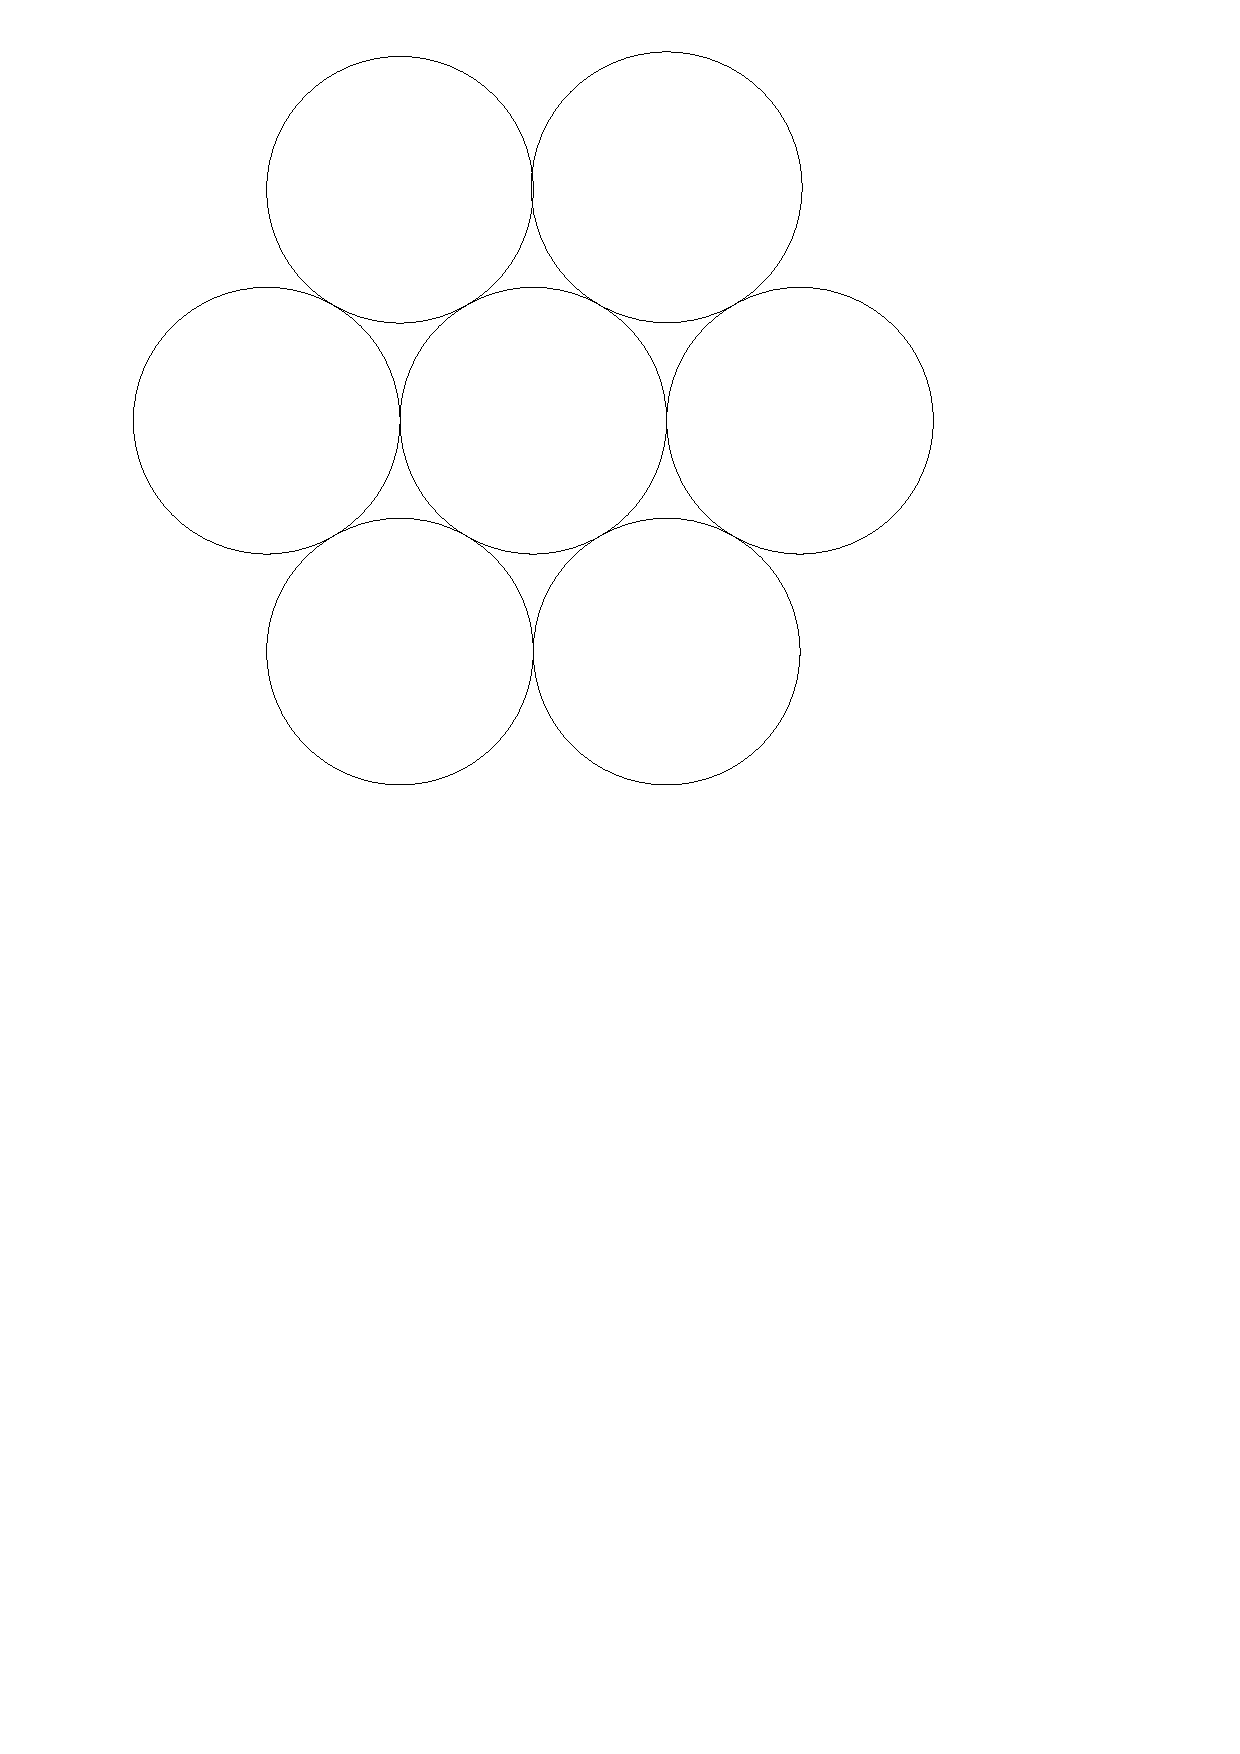
\includegraphics[width=.9\textwidth]{graphics/7ballLocked.pdf}
            \captionof{figure}{Caption Text}\label{gfx:7ballLocked.pdf}
            \end{center}
        \end{minipage}
    \end{columns}
\end{frame}
\begin{frame} \frametitle{7hexLocked.pdf}
    \begin{columns}[c]
    \column{.5\textwidth}
        \begin{itemize}
            \item[*] item 1
            \item[*] item 2
        \end{itemize}
    \column{.5\textwidth}
        \begin{minipage}{\linewidth}
            \begin{center}
            
\includegraphics[width=.9\textwidth]{graphics/7hexLocked.pdf}
            \captionof{figure}{Caption Text}\label{gfx:7hexLocked.pdf}
            \end{center}
        \end{minipage}
    \end{columns}
\end{frame}
\begin{frame} \frametitle{ActiveChannel.pdf}
    \begin{columns}[c]
    \column{.5\textwidth}
        \begin{itemize}
            \item[*] item 1
            \item[*] item 2
        \end{itemize}
    \column{.5\textwidth}
        \begin{minipage}{\linewidth}
            \begin{center}
            \includegraphics[width=.9\textwidth]{graphics/ActiveChannel.pdf}
            \captionof{figure}{Caption Text}\label{gfx:ActiveChannel.pdf}
            \end{center}
        \end{minipage}
    \end{columns}
\end{frame}
\begin{frame} \frametitle{AnatomyOfPerturbedSpine.pdf}
    \begin{columns}[c]
    \column{.5\textwidth}
        \begin{itemize}
            \item[*] item 1
            \item[*] item 2
        \end{itemize}
    \column{.5\textwidth}
        \begin{minipage}{\linewidth}
            \begin{center}
            \includegraphics[width=.9\textwidth]{graphics/AnatomyOfPerturbedSpine.pdf}
            \captionof{figure}{Caption Text}\label{gfx:AnatomyOfPerturbedSpine.pdf}
            \end{center}
        \end{minipage}
    \end{columns}
\end{frame}
\begin{frame} \frametitle{AngularDisplacement.pdf}
    \begin{columns}[c]
    \column{.5\textwidth}
        \begin{itemize}
            \item[*] item 1
            \item[*] item 2
        \end{itemize}
    \column{.5\textwidth}
        \begin{minipage}{\linewidth}
            \begin{center}
            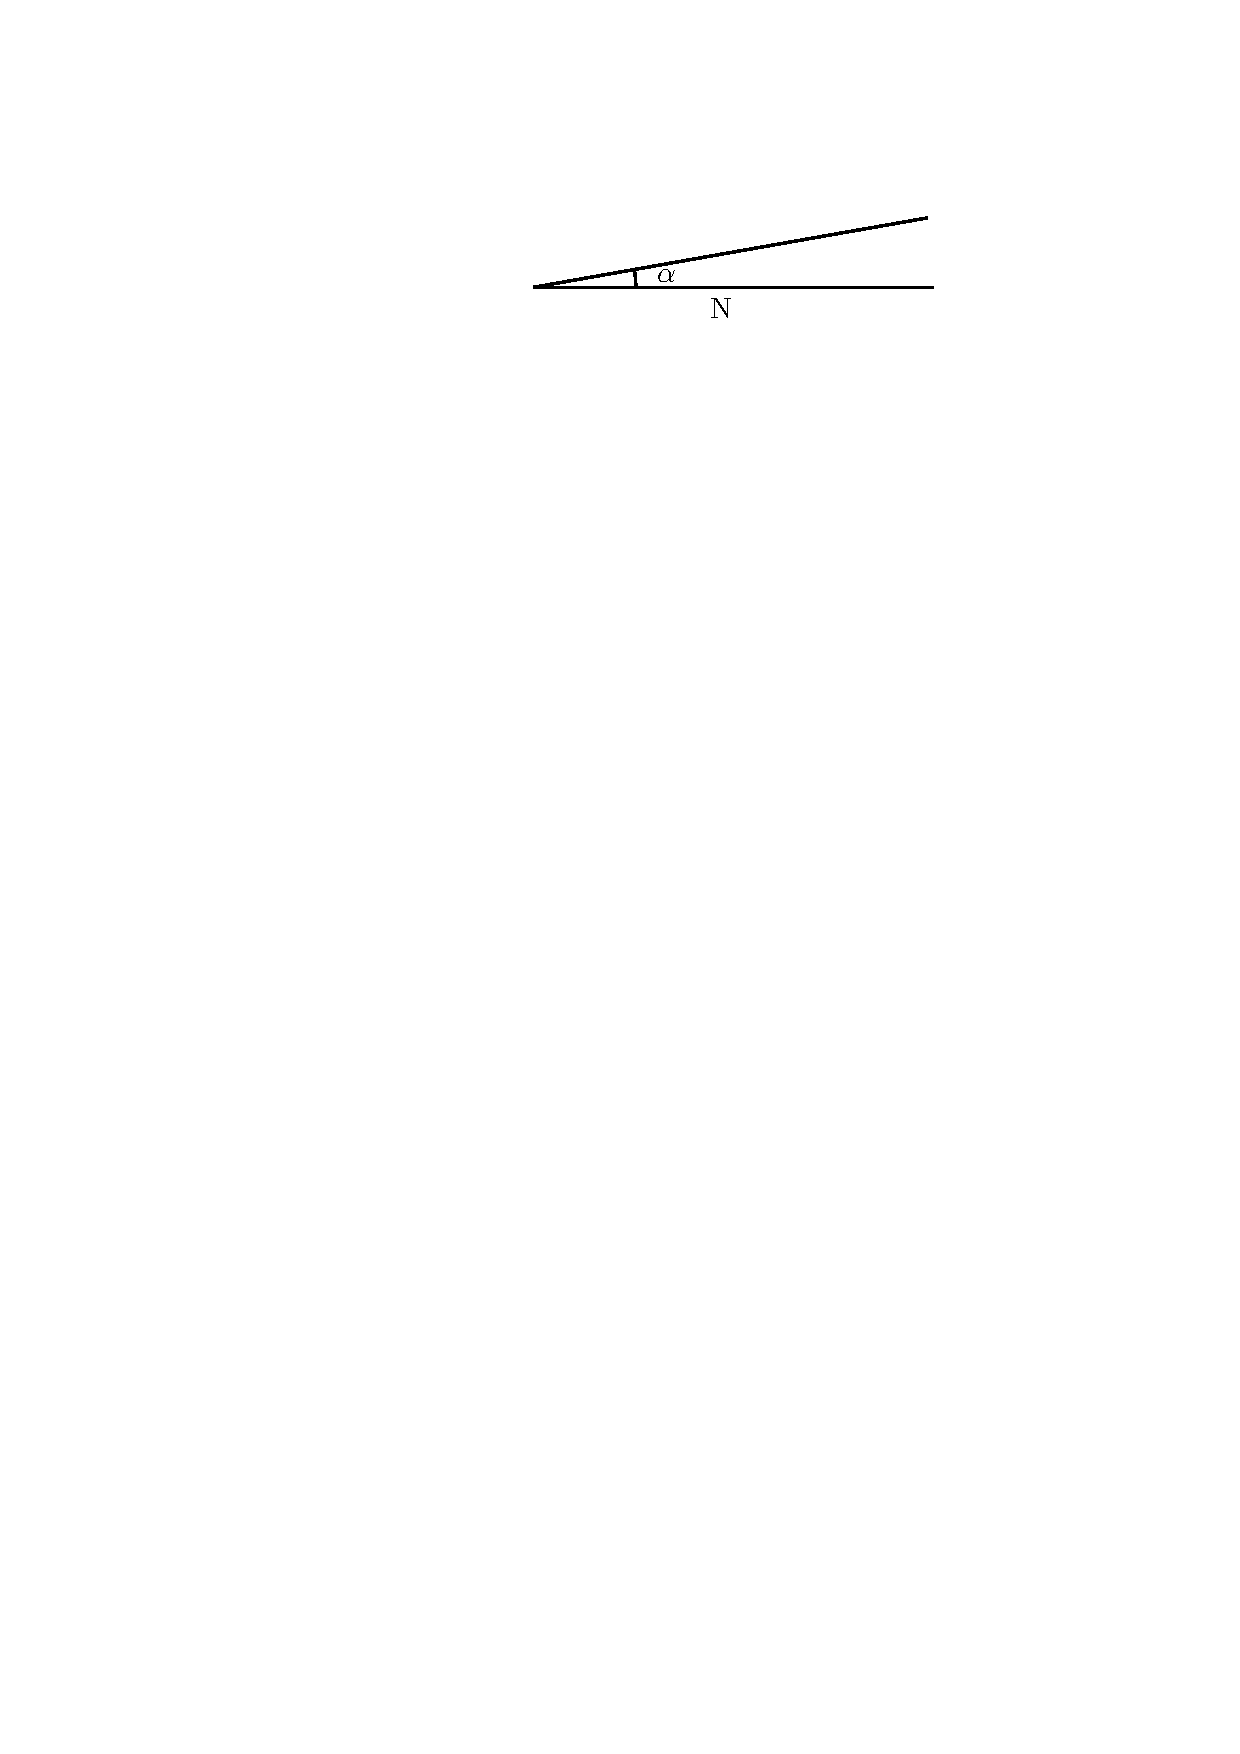
\includegraphics[width=.9\textwidth]{graphics/AngularDisplacement.pdf}
            \captionof{figure}{Caption Text}\label{gfx:AngularDisplacement.pdf}
            \end{center}
        \end{minipage}
    \end{columns}
\end{frame}
\begin{frame} \frametitle{betaOmegaFigure.pdf}
    \begin{columns}[c]
    \column{.5\textwidth}
        \begin{itemize}
            \item[*] item 1
            \item[*] item 2
        \end{itemize}
    \column{.5\textwidth}
        \begin{minipage}{\linewidth}
            \begin{center}
            \includegraphics[width=.9\textwidth]{graphics/betaOmegaFigure.pdf}
            \captionof{figure}{Caption Text}\label{gfx:betaOmegaFigure.pdf}
            \end{center}
        \end{minipage}
    \end{columns}
\end{frame}
\begin{frame} \frametitle{bigHexagonalGrid.pdf}
    \begin{columns}[c]
    \column{.5\textwidth}
        \begin{itemize}
            \item[*] item 1
            \item[*] item 2
        \end{itemize}
    \column{.5\textwidth}
        \begin{minipage}{\linewidth}
            \begin{center}
            \includegraphics[width=.9\textwidth]{graphics/bigHexagonalGrid.pdf}
            \captionof{figure}{Caption Text}\label{gfx:bigHexagonalGrid.pdf}
            \end{center}
        \end{minipage}
    \end{columns}
\end{frame}
\begin{frame} \frametitle{BinaryTree1.pdf}
    \begin{columns}[c]
    \column{.5\textwidth}
        \begin{itemize}
            \item[*] item 1
            \item[*] item 2
        \end{itemize}
    \column{.5\textwidth}
        \begin{minipage}{\linewidth}
            \begin{center}
            \includegraphics[width=.9\textwidth]{graphics/BinaryTree1.pdf}
            \captionof{figure}{Caption Text}\label{gfx:BinaryTree1.pdf}
            \end{center}
        \end{minipage}
    \end{columns}
\end{frame}
\begin{frame} \frametitle{BinaryTree2.pdf}
    \begin{columns}[c]
    \column{.5\textwidth}
        \begin{itemize}
            \item[*] item 1
            \item[*] item 2
        \end{itemize}
    \column{.5\textwidth}
        \begin{minipage}{\linewidth}
            \begin{center}
            \includegraphics[width=.9\textwidth]{graphics/BinaryTree2.pdf}
            \captionof{figure}{Caption Text}\label{gfx:BinaryTree2.pdf}
            \end{center}
        \end{minipage}
    \end{columns}
\end{frame}
\begin{frame} \frametitle{BinaryTree3.pdf}
    \begin{columns}[c]
    \column{.5\textwidth}
        \begin{itemize}
            \item[*] item 1
            \item[*] item 2
        \end{itemize}
    \column{.5\textwidth}
        \begin{minipage}{\linewidth}
            \begin{center}
            \includegraphics[width=.9\textwidth]{graphics/BinaryTree3.pdf}
            \captionof{figure}{Caption Text}\label{gfx:BinaryTree3.pdf}
            \end{center}
        \end{minipage}
    \end{columns}
\end{frame}
\begin{frame} \frametitle{BinaryTree4.pdf}
    \begin{columns}[c]
    \column{.5\textwidth}
        \begin{itemize}
            \item[*] item 1
            \item[*] item 2
        \end{itemize}
    \column{.5\textwidth}
        \begin{minipage}{\linewidth}
            \begin{center}
            \includegraphics[width=.9\textwidth]{graphics/BinaryTree4.pdf}
            \captionof{figure}{Caption Text}\label{gfx:BinaryTree4.pdf}
            \end{center}
        \end{minipage}
    \end{columns}
\end{frame}
\begin{frame} \frametitle{block3c.pdf}
    \begin{columns}[c]
    \column{.5\textwidth}
        \begin{itemize}
            \item[*] item 1
            \item[*] item 2
        \end{itemize}
    \column{.5\textwidth}
        \begin{minipage}{\linewidth}
            \begin{center}
            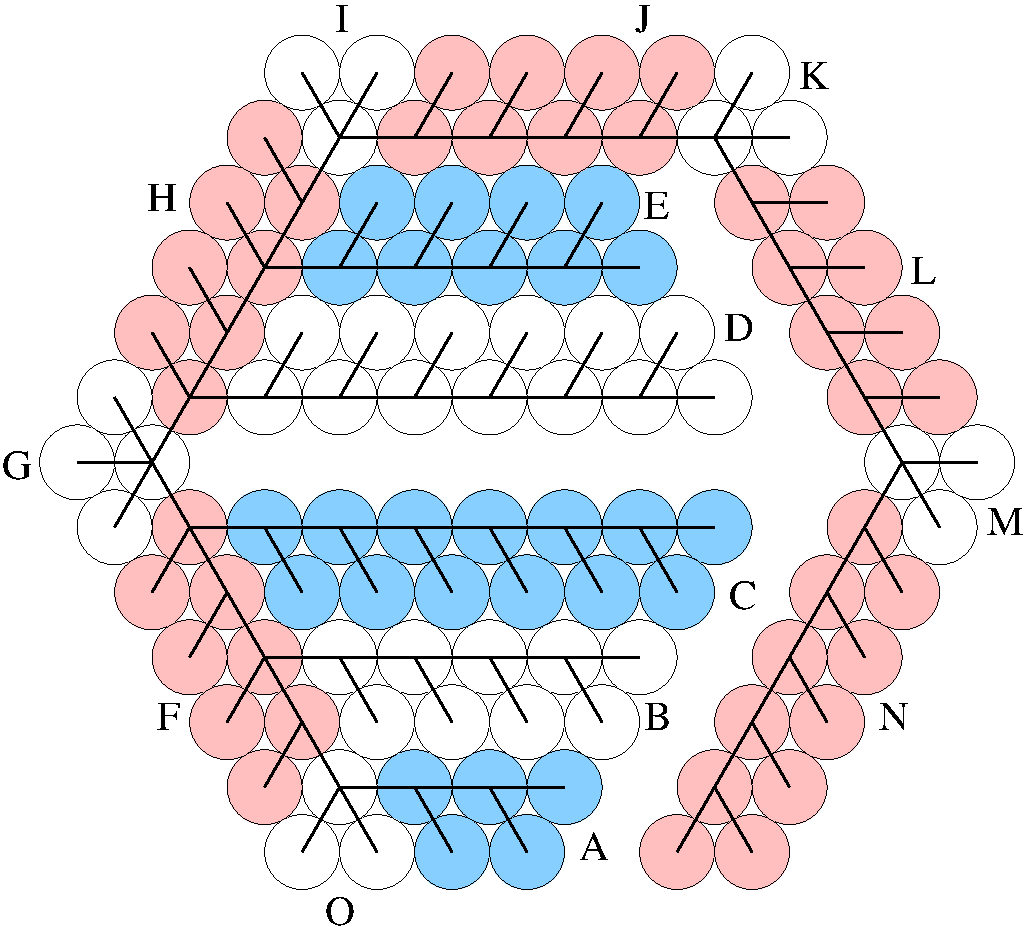
\includegraphics[width=.9\textwidth]{graphics/block3c.pdf}
            \captionof{figure}{Caption Text}\label{gfx:block3c.pdf}
            \end{center}
        \end{minipage}
    \end{columns}
\end{frame}
\begin{frame} \frametitle{BottomOfJ.pdf}
    \begin{columns}[c]
    \column{.5\textwidth}
        \begin{itemize}
            \item[*] item 1
            \item[*] item 2
        \end{itemize}
    \column{.5\textwidth}
        \begin{minipage}{\linewidth}
            \begin{center}
            \includegraphics[width=.9\textwidth]{graphics/BottomOfJ.pdf}
            \captionof{figure}{Caption Text}\label{gfx:BottomOfJ.pdf}
            \end{center}
        \end{minipage}
    \end{columns}
\end{frame}
\begin{frame} \frametitle{ch4Paralellogram.pdf}
    \begin{columns}[c]
    \column{.5\textwidth}
        \begin{itemize}
            \item[*] item 1
            \item[*] item 2
        \end{itemize}
    \column{.5\textwidth}
        \begin{minipage}{\linewidth}
            \begin{center}
            \includegraphics[width=.9\textwidth]{graphics/ch4Paralellogram.pdf}
            \captionof{figure}{Caption Text}\label{gfx:ch4Paralellogram.pdf}
            \end{center}
        \end{minipage}
    \end{columns}
\end{frame}
\begin{frame} \frametitle{circlePackingEdgeRepressentingKissingPoints.pdf}
    \begin{columns}[c]
    \column{.5\textwidth}
        \begin{itemize}
            \item[*] item 1
            \item[*] item 2
        \end{itemize}
    \column{.5\textwidth}
        \begin{minipage}{\linewidth}
            \begin{center}
            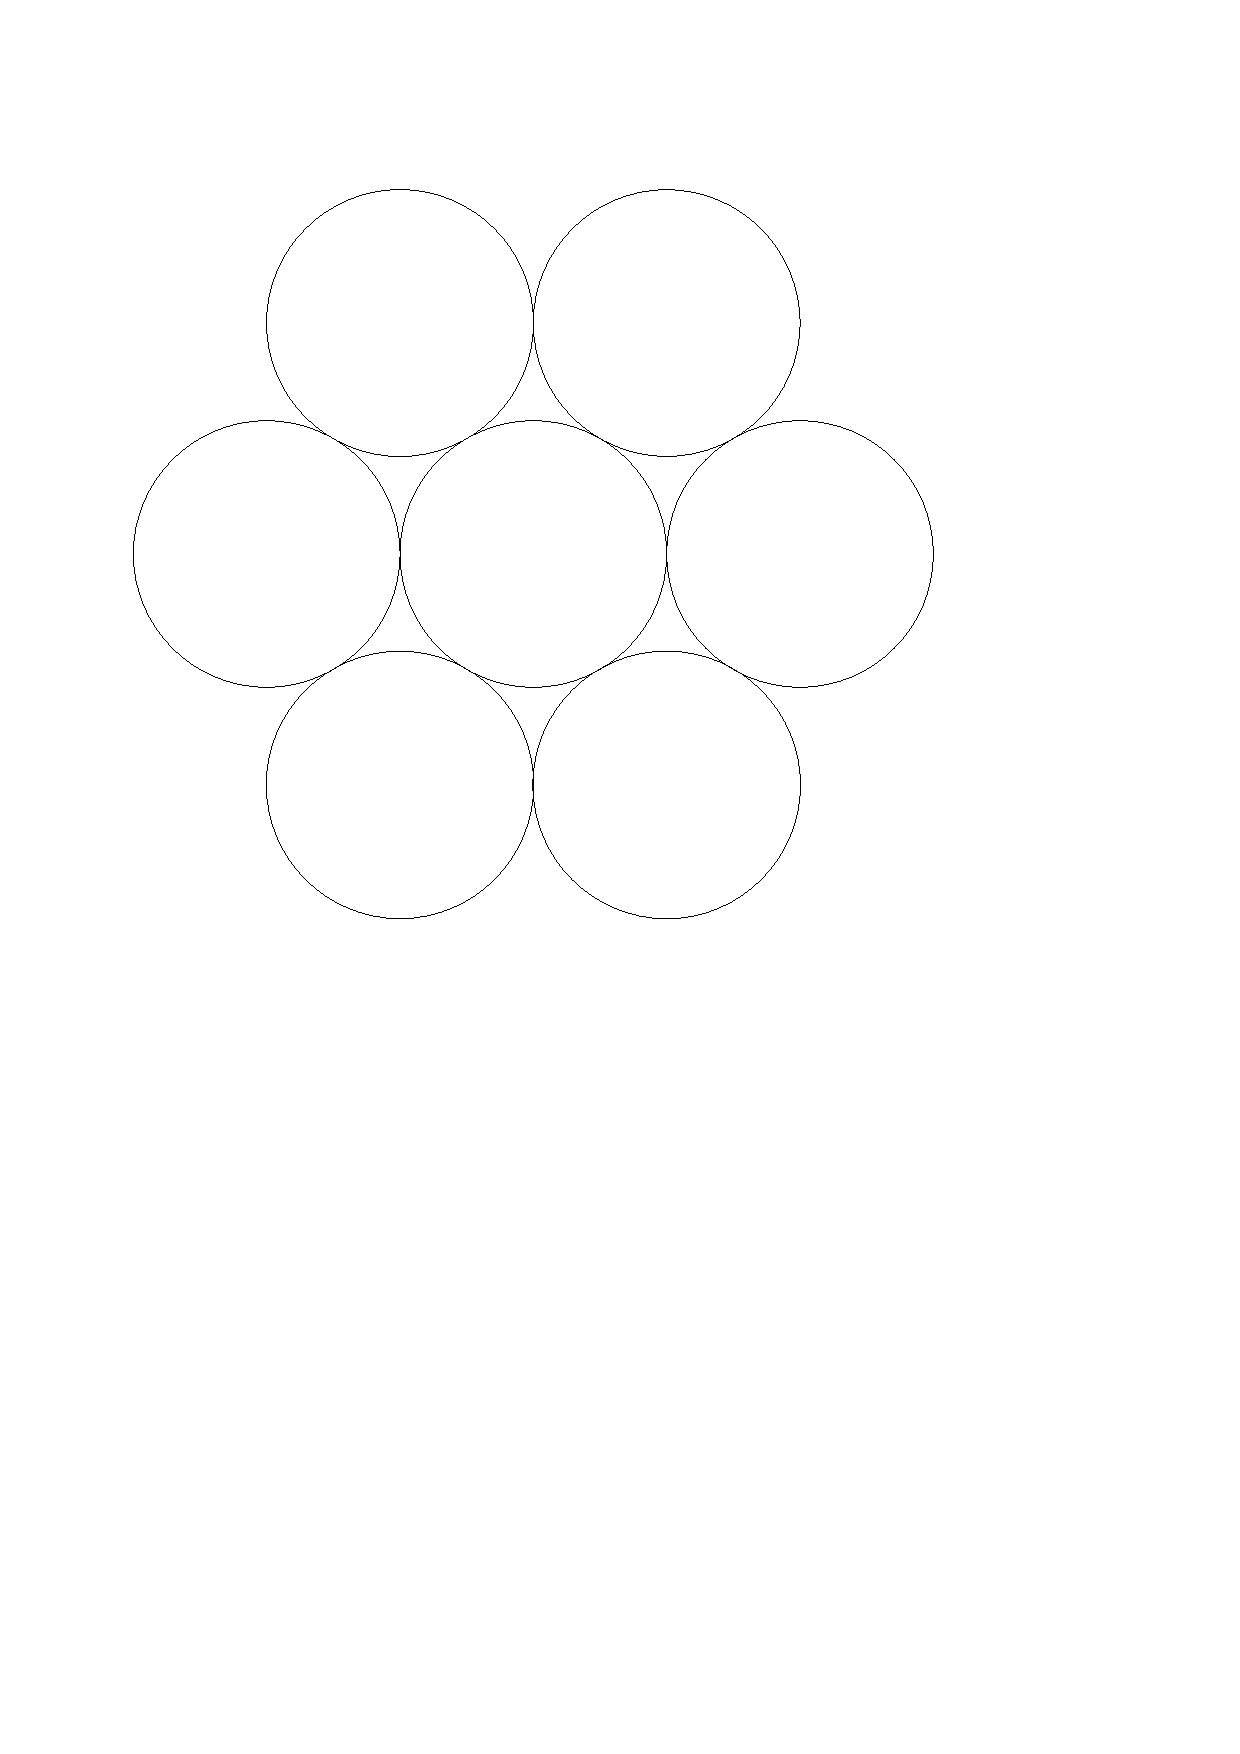
\includegraphics[width=.9\textwidth]{graphics/circlePackingEdgeRepressentingKissingPoints.pdf}
            \captionof{figure}{Caption Text}\label{gfx:circlePackingEdgeRepressentingKissingPoints.pdf}
            \end{center}
        \end{minipage}
    \end{columns}
\end{frame}
\begin{frame} \frametitle{circlePackingTheoremExample.pdf}
    \begin{columns}[c]
    \column{.5\textwidth}
        \begin{itemize}
            \item[*] item 1
            \item[*] item 2
        \end{itemize}
    \column{.5\textwidth}
        \begin{minipage}{\linewidth}
            \begin{center}
            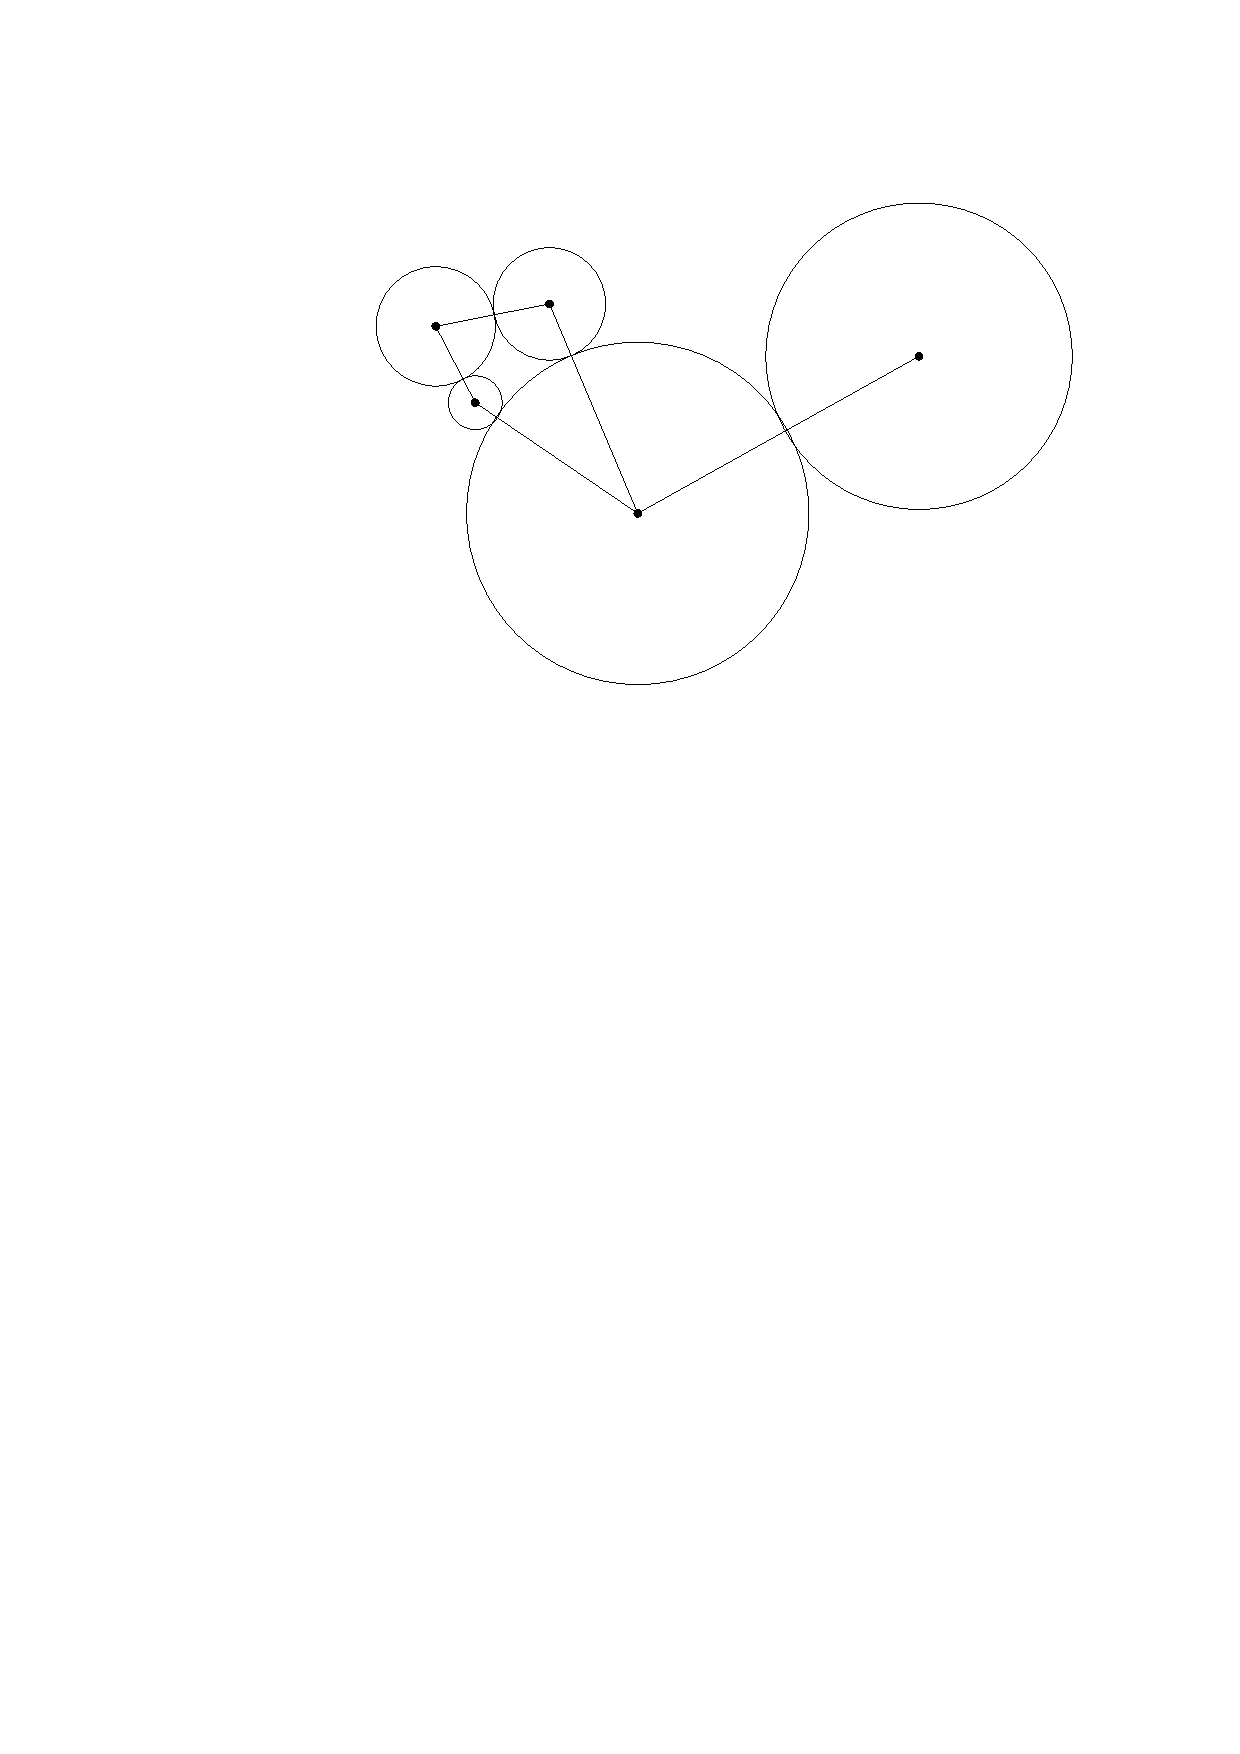
\includegraphics[width=.9\textwidth]{graphics/circlePackingTheoremExample.pdf}
            \captionof{figure}{Caption Text}\label{gfx:circlePackingTheoremExample.pdf}
            \end{center}
        \end{minipage}
    \end{columns}
\end{frame}
\begin{frame} \frametitle{circumscribedHexagon.pdf}
    \begin{columns}[c]
    \column{.5\textwidth}
        \begin{itemize}
            \item[*] item 1
            \item[*] item 2
        \end{itemize}
    \column{.5\textwidth}
        \begin{minipage}{\linewidth}
            \begin{center}
            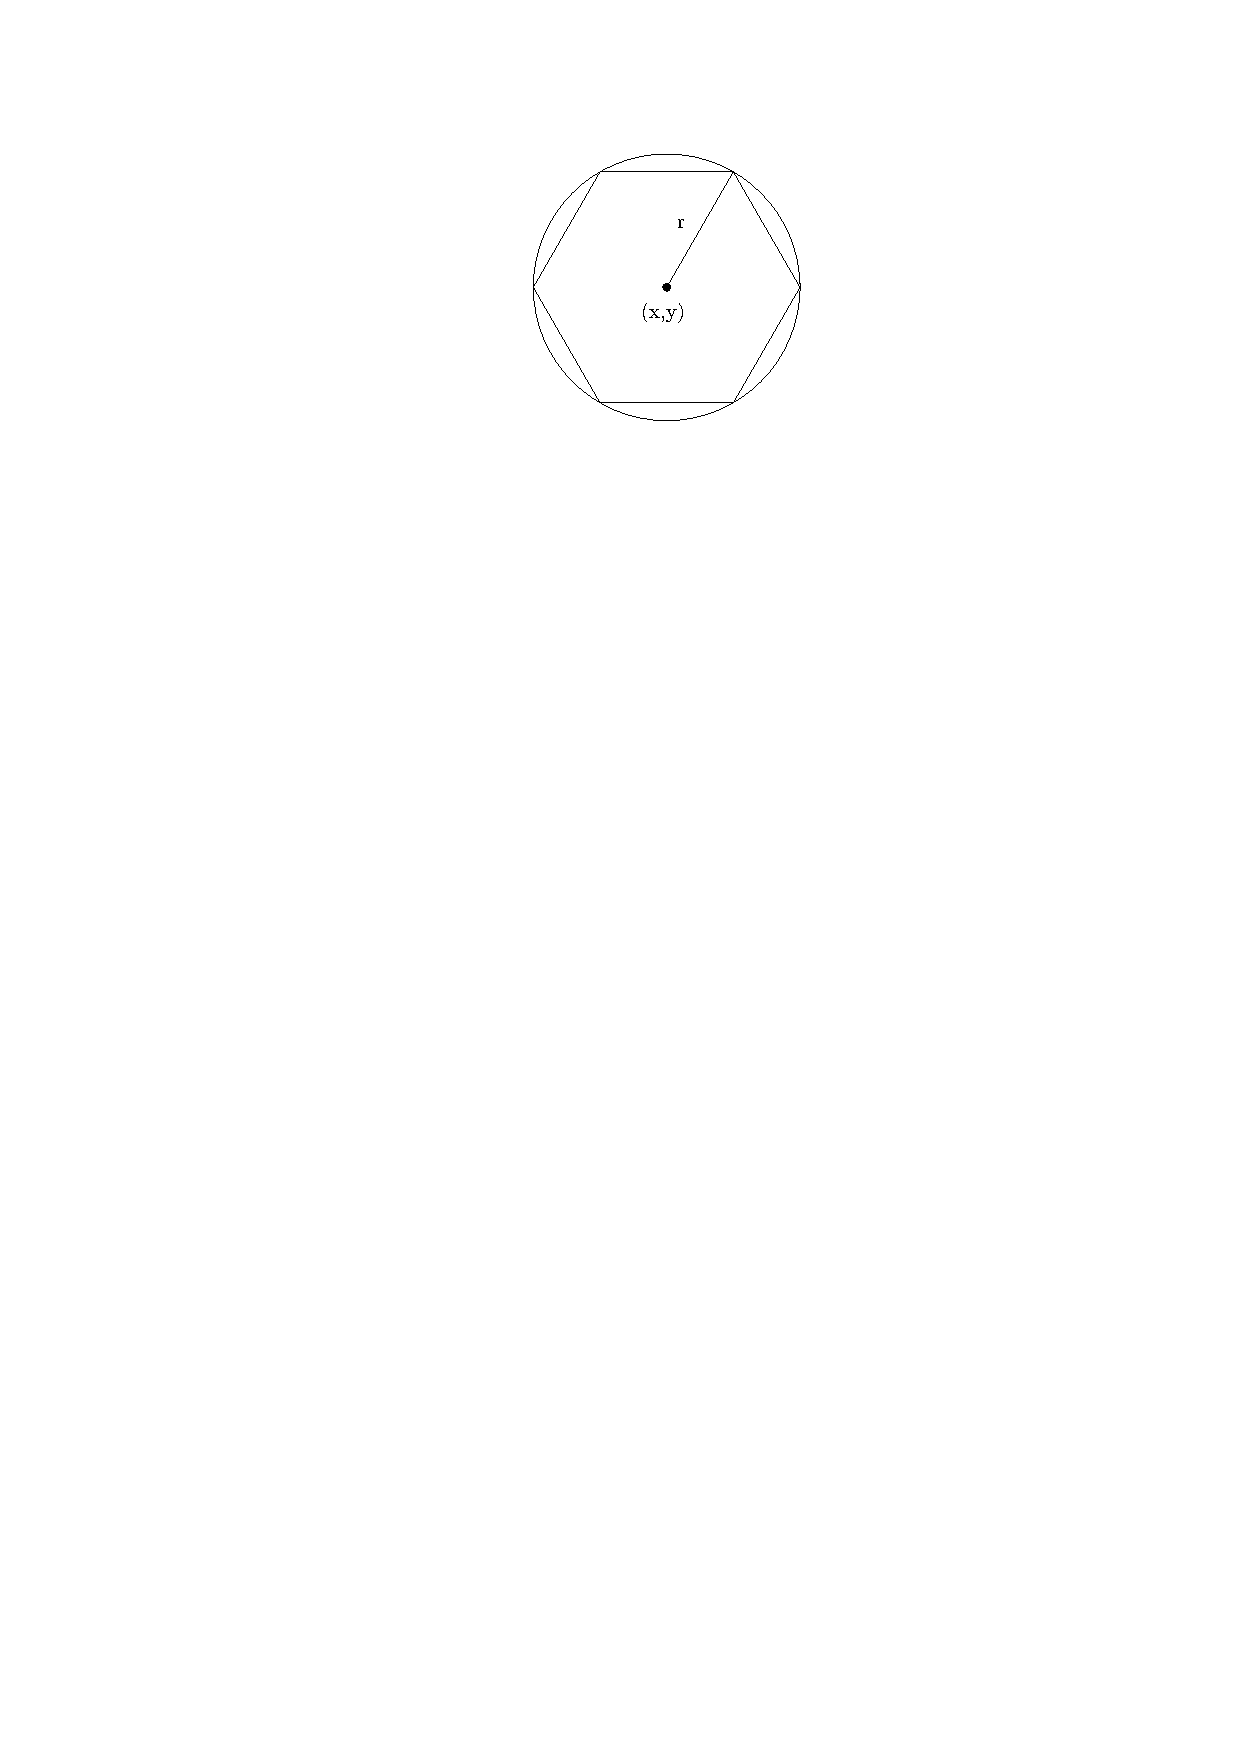
\includegraphics[width=.9\textwidth]{graphics/circumscribedHexagon.pdf}
            \captionof{figure}{Caption Text}\label{gfx:circumscribedHexagon.pdf}
            \end{center}
        \end{minipage}
    \end{columns}
\end{frame}
\begin{frame} \frametitle{collidingHingedPolygons.pdf}
    \begin{columns}[c]
    \column{.5\textwidth}
        \begin{itemize}
            \item[*] item 1
            \item[*] item 2
        \end{itemize}
    \column{.5\textwidth}
        \begin{minipage}{\linewidth}
            \begin{center}
            \includegraphics[width=.9\textwidth]{graphics/collidingHingedPolygons.pdf}
            \captionof{figure}{Caption Text}\label{gfx:collidingHingedPolygons.pdf}
            \end{center}
        \end{minipage}
    \end{columns}
\end{frame}
\begin{frame} \frametitle{combinatorialEmbedding.pdf}
    \begin{columns}[c]
    \column{.5\textwidth}
        \begin{itemize}
            \item[*] item 1
            \item[*] item 2
        \end{itemize}
    \column{.5\textwidth}
        \begin{minipage}{\linewidth}
            \begin{center}
            \includegraphics[width=.9\textwidth]{graphics/combinatorialEmbedding.pdf}
            \captionof{figure}{Caption Text}\label{gfx:combinatorialEmbedding.pdf}
            \end{center}
        \end{minipage}
    \end{columns}
\end{frame}
\begin{frame} \frametitle{corridorNonCanonical.pdf}
    \begin{columns}[c]
    \column{.5\textwidth}
        \begin{itemize}
            \item[*] item 1
            \item[*] item 2
        \end{itemize}
    \column{.5\textwidth}
        \begin{minipage}{\linewidth}
            \begin{center}
            \includegraphics[width=.9\textwidth]{graphics/corridorNonCanonical.pdf}
            \captionof{figure}{Caption Text}\label{gfx:corridorNonCanonical.pdf}
            \end{center}
        \end{minipage}
    \end{columns}
\end{frame}
\begin{frame} \frametitle{corridorNonCanonical2.pdf}
    \begin{columns}[c]
    \column{.5\textwidth}
        \begin{itemize}
            \item[*] item 1
            \item[*] item 2
        \end{itemize}
    \column{.5\textwidth}
        \begin{minipage}{\linewidth}
            \begin{center}
            \includegraphics[width=.9\textwidth]{graphics/corridorNonCanonical2.pdf}
            \captionof{figure}{Caption Text}\label{gfx:corridorNonCanonical2.pdf}
            \end{center}
        \end{minipage}
    \end{columns}
\end{frame}
\begin{frame} \frametitle{crossingEdgeLinkage.pdf}
    \begin{columns}[c]
    \column{.5\textwidth}
        \begin{itemize}
            \item[*] item 1
            \item[*] item 2
        \end{itemize}
    \column{.5\textwidth}
        \begin{minipage}{\linewidth}
            \begin{center}
            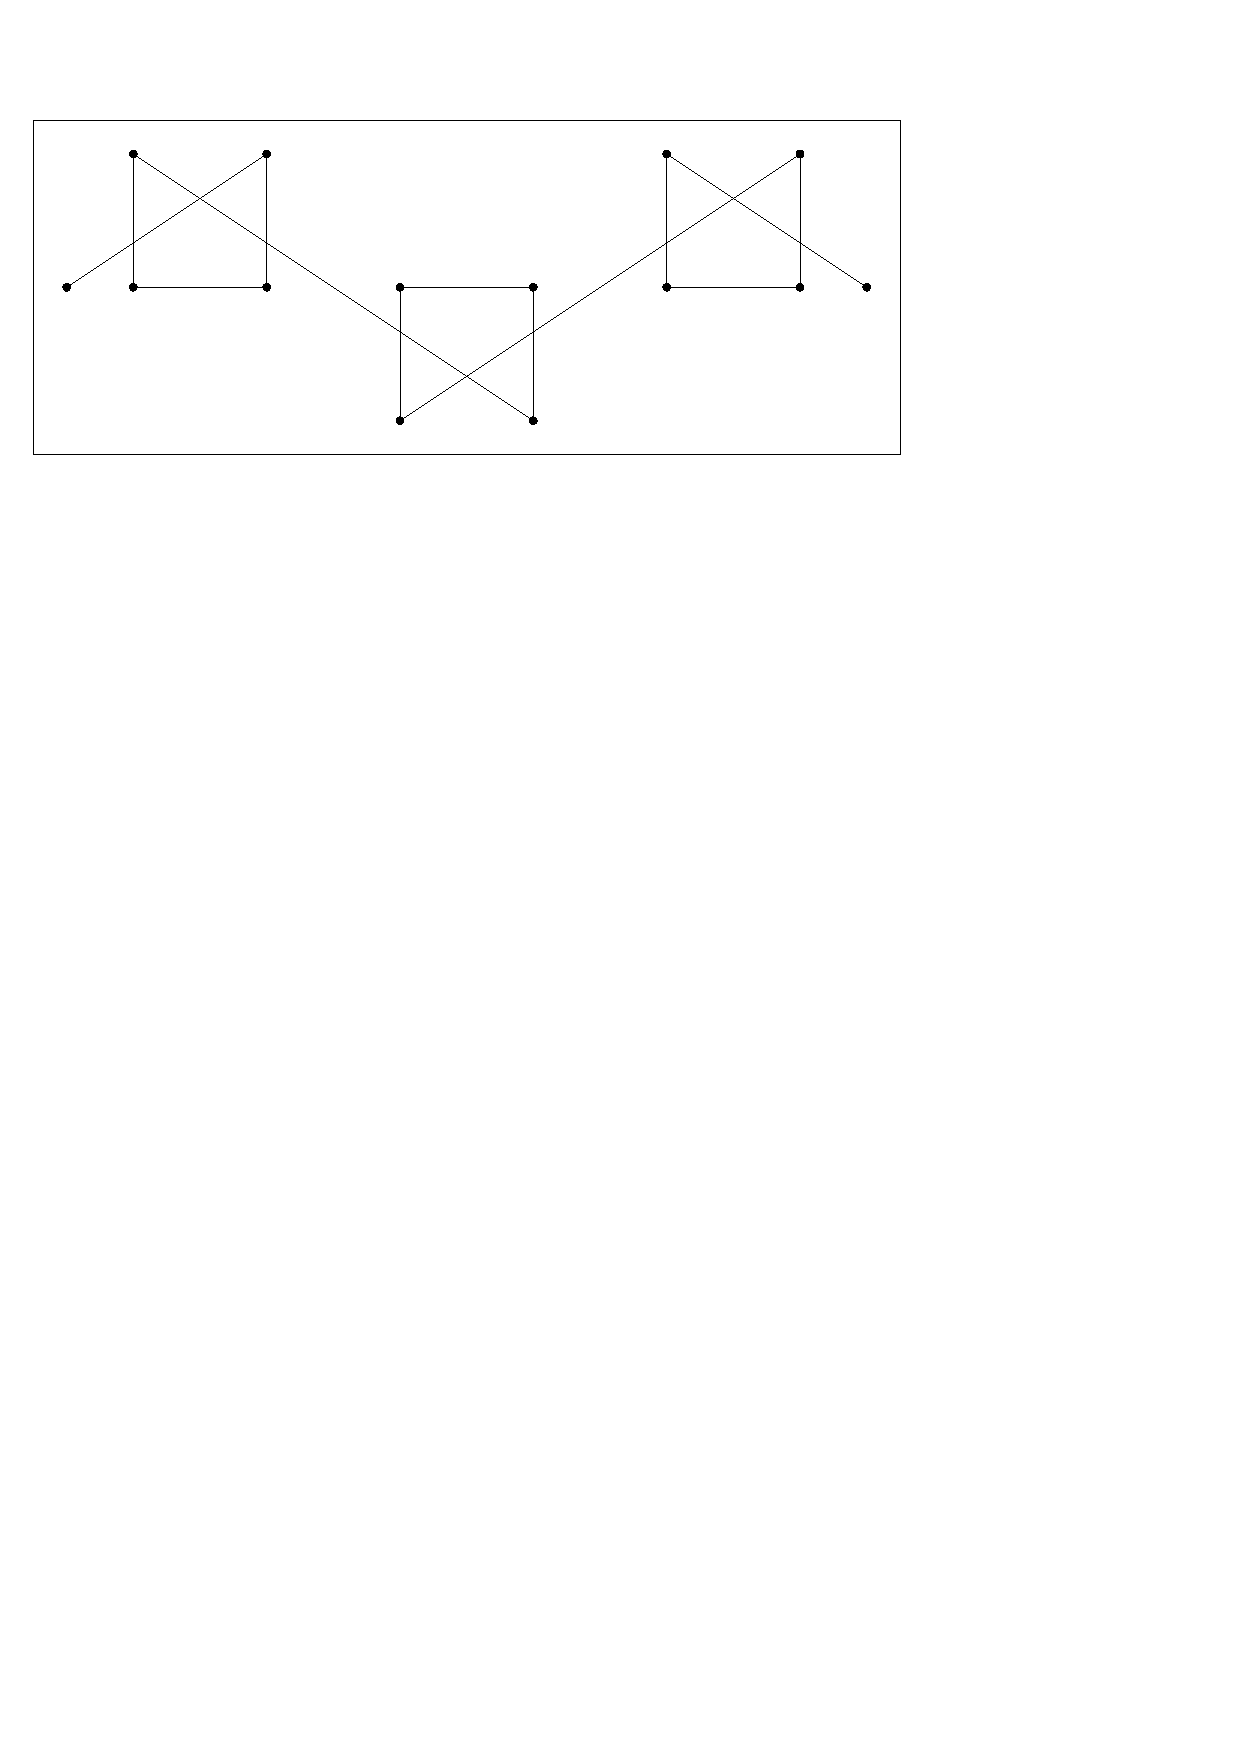
\includegraphics[width=.9\textwidth]{graphics/crossingEdgeLinkage.pdf}
            \captionof{figure}{Caption Text}\label{gfx:crossingEdgeLinkage.pdf}
            \end{center}
        \end{minipage}
    \end{columns}
\end{frame}
\begin{frame} \frametitle{crossingType2.pdf}
    \begin{columns}[c]
    \column{.5\textwidth}
        \begin{itemize}
            \item[*] item 1
            \item[*] item 2
        \end{itemize}
    \column{.5\textwidth}
        \begin{minipage}{\linewidth}
            \begin{center}
            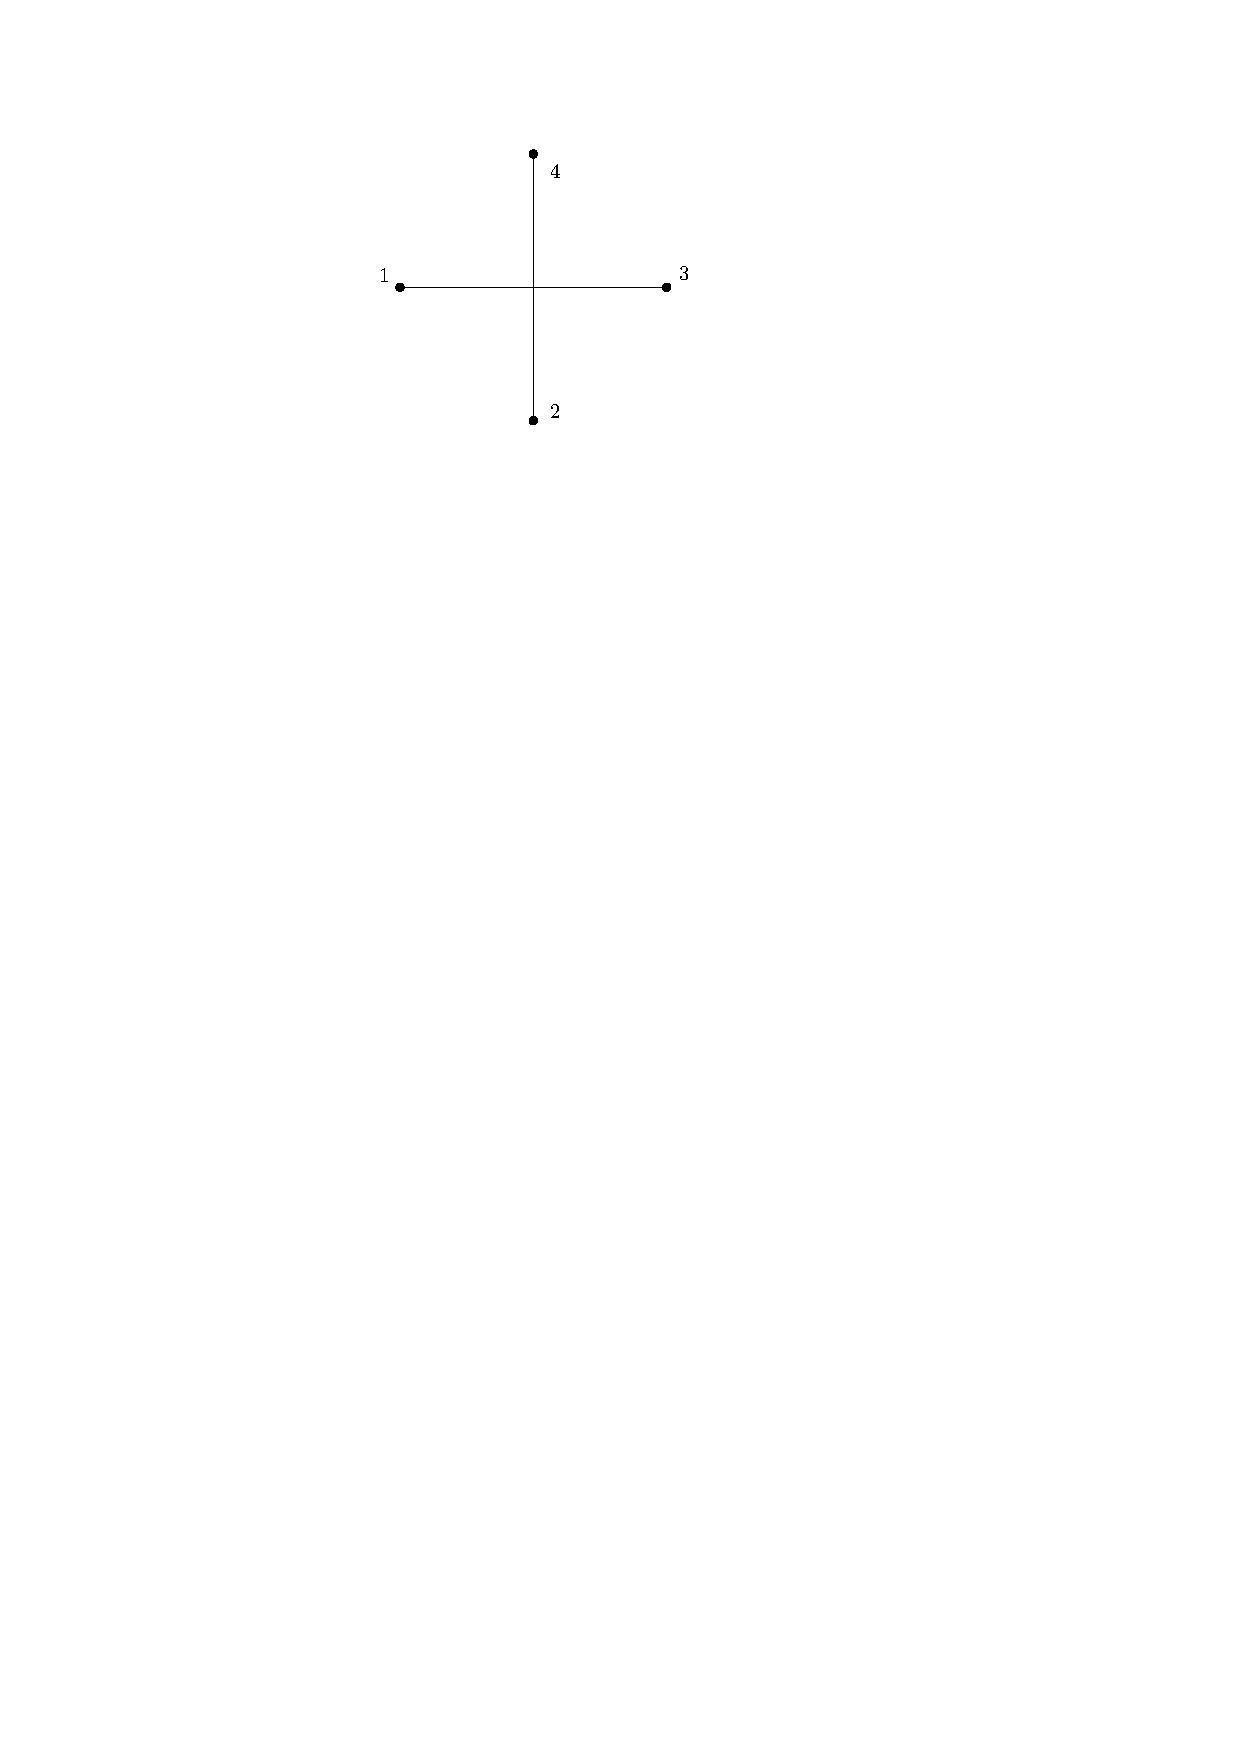
\includegraphics[width=.9\textwidth]{graphics/crossingType2.pdf}
            \captionof{figure}{Caption Text}\label{gfx:crossingType2.pdf}
            \end{center}
        \end{minipage}
    \end{columns}
\end{frame}
\begin{frame} \frametitle{crossingType3.pdf}
    \begin{columns}[c]
    \column{.5\textwidth}
        \begin{itemize}
            \item[*] item 1
            \item[*] item 2
        \end{itemize}
    \column{.5\textwidth}
        \begin{minipage}{\linewidth}
            \begin{center}
            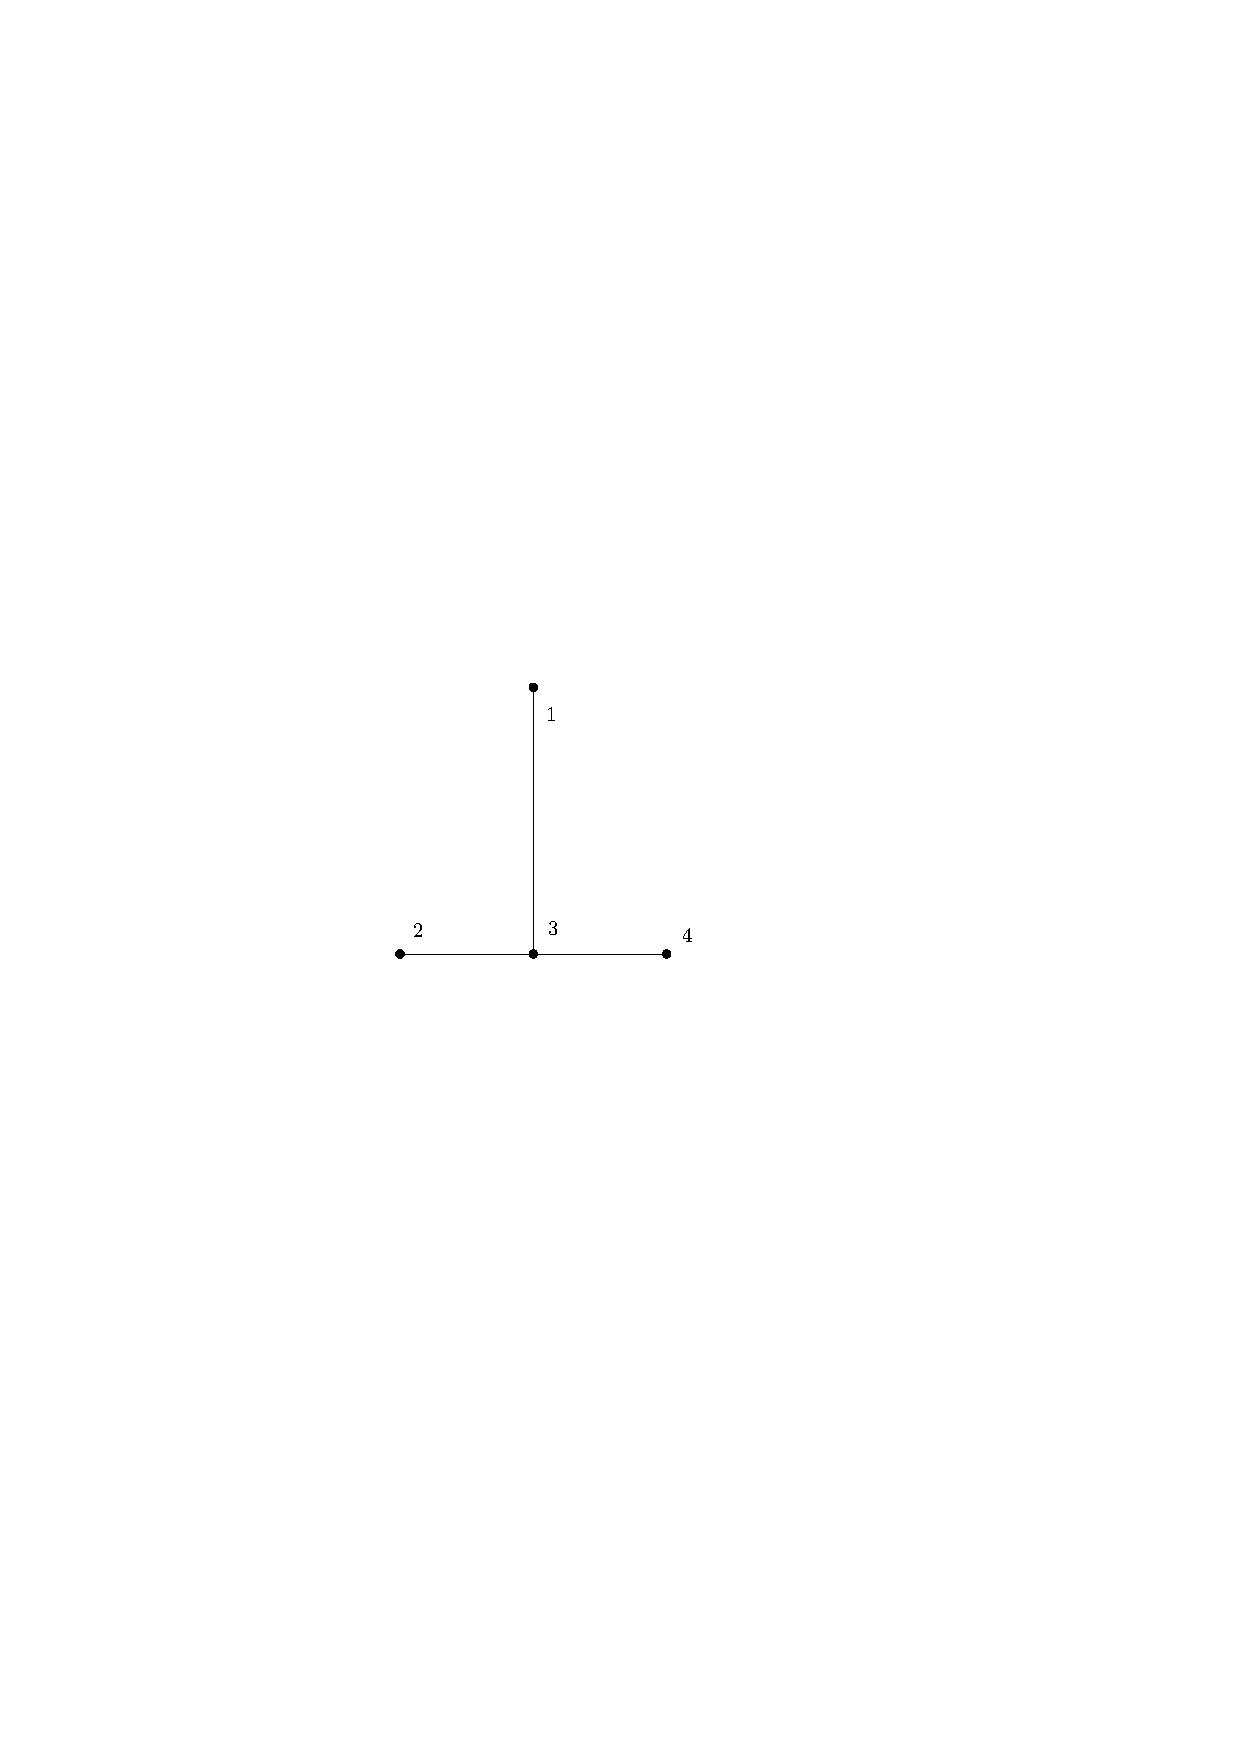
\includegraphics[width=.9\textwidth]{graphics/crossingType3.pdf}
            \captionof{figure}{Caption Text}\label{gfx:crossingType3.pdf}
            \end{center}
        \end{minipage}
    \end{columns}
\end{frame}
\begin{frame} \frametitle{CrossSection.pdf}
    \begin{columns}[c]
    \column{.5\textwidth}
        \begin{itemize}
            \item[*] item 1
            \item[*] item 2
        \end{itemize}
    \column{.5\textwidth}
        \begin{minipage}{\linewidth}
            \begin{center}
            \includegraphics[width=.9\textwidth]{graphics/CrossSection.pdf}
            \captionof{figure}{Caption Text}\label{gfx:CrossSection.pdf}
            \end{center}
        \end{minipage}
    \end{columns}
\end{frame}
\begin{frame} \frametitle{CrossSectionArea.pdf}
    \begin{columns}[c]
    \column{.5\textwidth}
        \begin{itemize}
            \item[*] item 1
            \item[*] item 2
        \end{itemize}
    \column{.5\textwidth}
        \begin{minipage}{\linewidth}
            \begin{center}
            \includegraphics[width=.9\textwidth]{graphics/CrossSectionArea.pdf}
            \captionof{figure}{Caption Text}\label{gfx:CrossSectionArea.pdf}
            \end{center}
        \end{minipage}
    \end{columns}
\end{frame}
\begin{frame} \frametitle{D1.pdf}
    \begin{columns}[c]
    \column{.5\textwidth}
        \begin{itemize}
            \item[*] item 1
            \item[*] item 2
        \end{itemize}
    \column{.5\textwidth}
        \begin{minipage}{\linewidth}
            \begin{center}
            \includegraphics[width=.9\textwidth]{graphics/D1.pdf}
            \captionof{figure}{Caption Text}\label{gfx:D1.pdf}
            \end{center}
        \end{minipage}
    \end{columns}
\end{frame}
\begin{frame} \frametitle{degree2arrangement.pdf}
    \begin{columns}[c]
    \column{.5\textwidth}
        \begin{itemize}
            \item[*] item 1
            \item[*] item 2
        \end{itemize}
    \column{.5\textwidth}
        \begin{minipage}{\linewidth}
            \begin{center}
            
\includegraphics[width=.9\textwidth]{graphics/degree2arrangement.pdf}
            \captionof{figure}{Caption Text}\label{gfx:degree2arrangement.pdf}
            \end{center}
        \end{minipage}
    \end{columns}
\end{frame}
\begin{frame} \frametitle{degree3arrangement.pdf}
    \begin{columns}[c]
    \column{.5\textwidth}
        \begin{itemize}
            \item[*] item 1
            \item[*] item 2
        \end{itemize}
    \column{.5\textwidth}
        \begin{minipage}{\linewidth}
            \begin{center}
            
\includegraphics[width=.9\textwidth]{graphics/degree3arrangement.pdf}
            \captionof{figure}{Caption Text}\label{gfx:degree3arrangement.pdf}
            \end{center}
        \end{minipage}
    \end{columns}
\end{frame}
\begin{frame} \frametitle{degree4arrangement.pdf}
    \begin{columns}[c]
    \column{.5\textwidth}
        \begin{itemize}
            \item[*] item 1
            \item[*] item 2
        \end{itemize}
    \column{.5\textwidth}
        \begin{minipage}{\linewidth}
            \begin{center}
            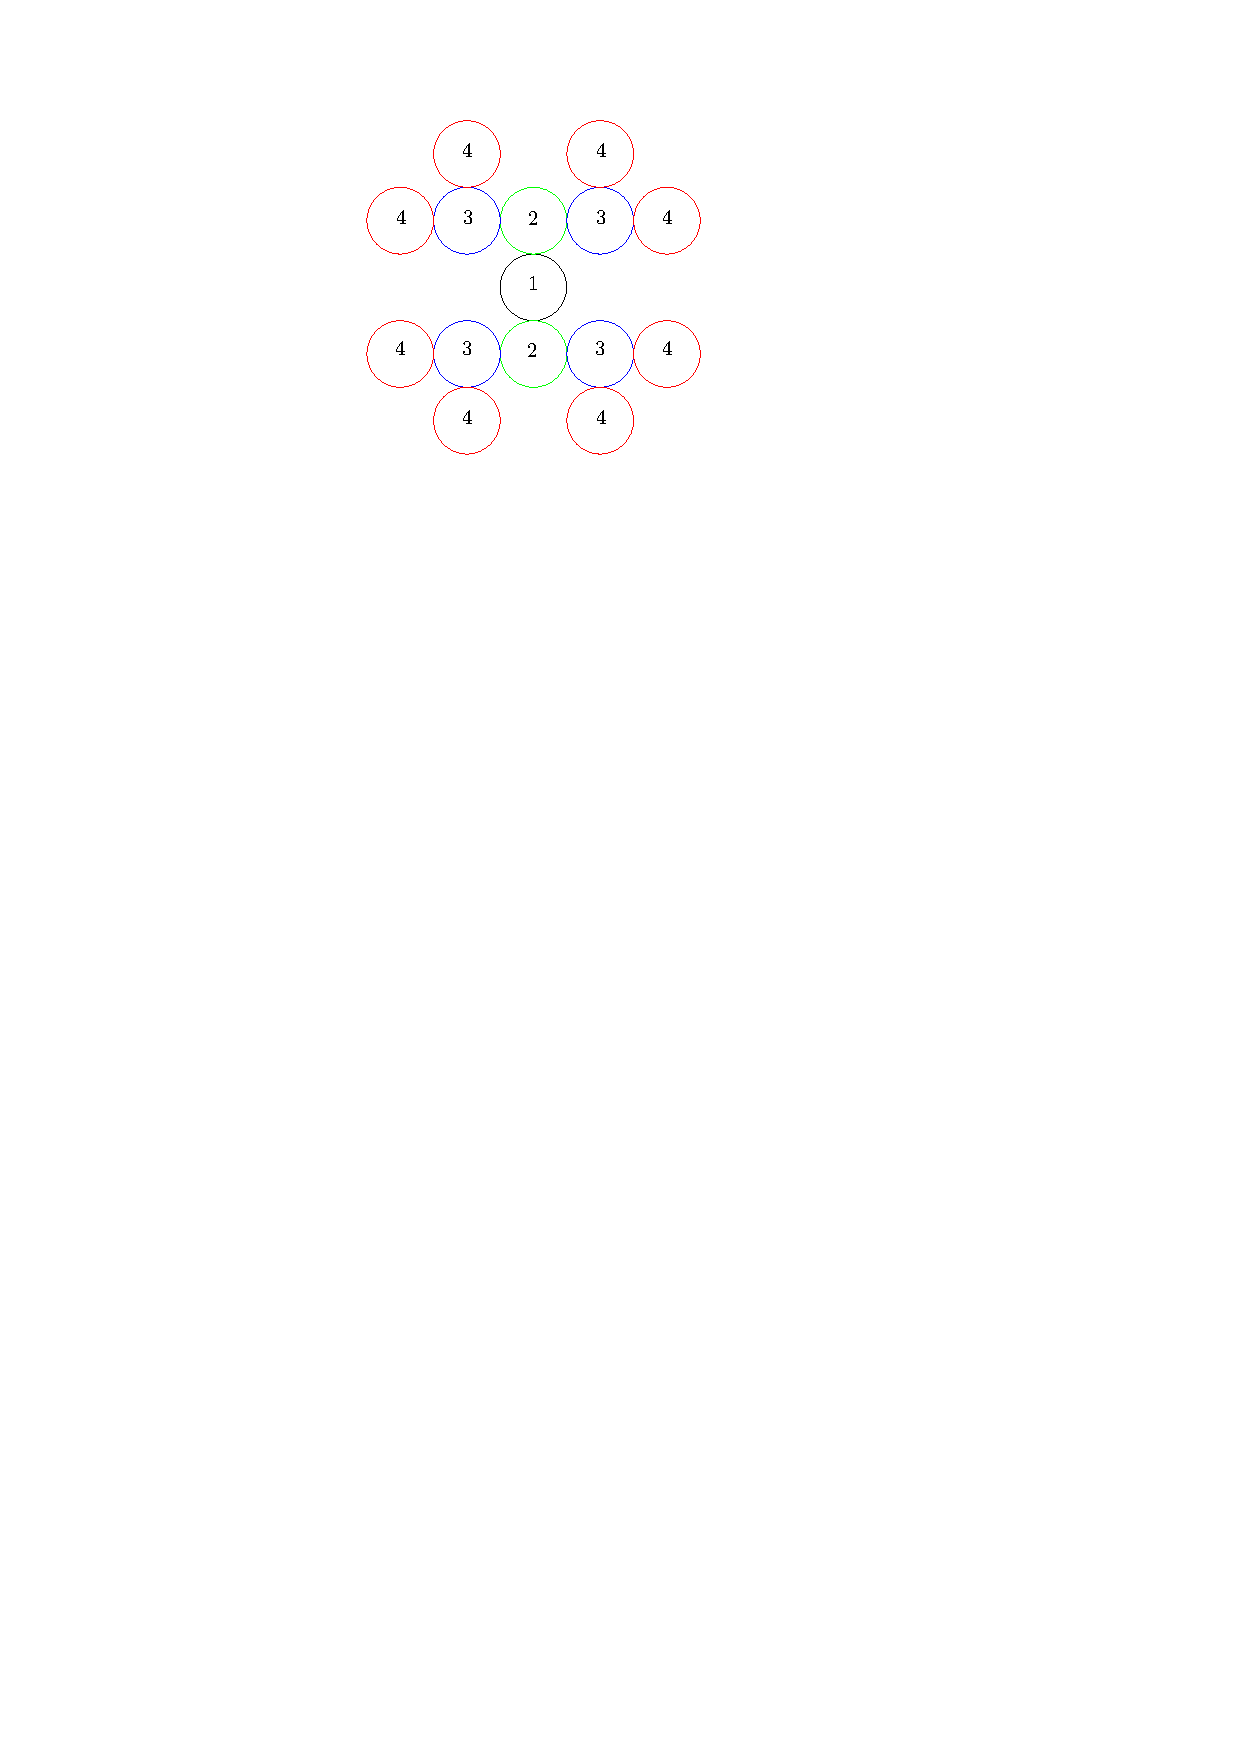
\includegraphics[width=.9\textwidth]{graphics/degree4arrangement.pdf}
            \captionof{figure}{Caption Text}\label{gfx:degree4arrangement.pdf}
            \end{center}
        \end{minipage}
    \end{columns}
\end{frame}
\begin{frame} \frametitle{degree5arrangement.pdf}
    \begin{columns}[c]
    \column{.5\textwidth}
        \begin{itemize}
            \item[*] item 1
            \item[*] item 2
        \end{itemize}
    \column{.5\textwidth}
        \begin{minipage}{\linewidth}
            \begin{center}
            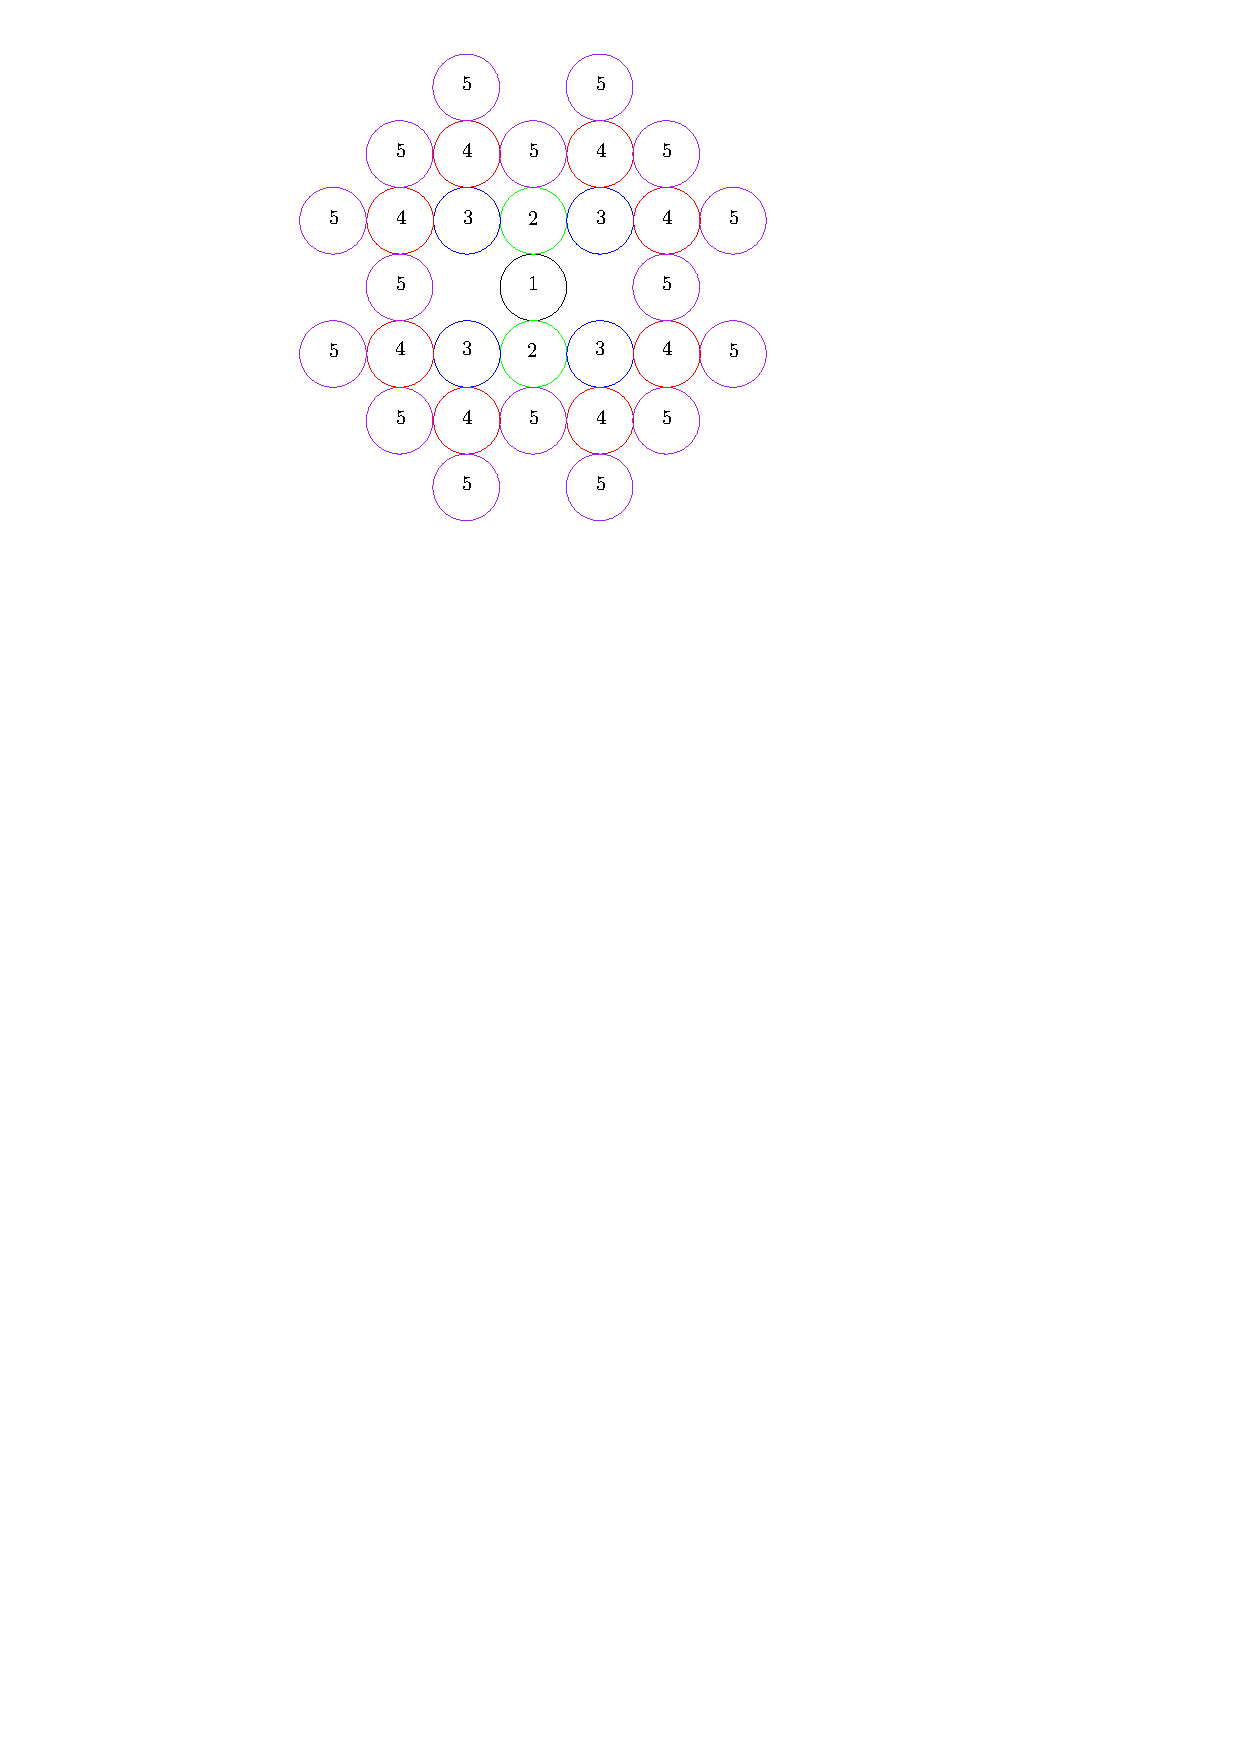
\includegraphics[width=.9\textwidth]{graphics/degree5arrangement.pdf}
            \captionof{figure}{Caption Text}\label{gfx:degree5arrangement.pdf}
            \end{center}
        \end{minipage}
    \end{columns}
\end{frame}
\begin{frame} \frametitle{deltaAlphaHorizontalDisplacement.pdf}
    \begin{columns}[c]
    \column{.5\textwidth}
        \begin{itemize}
            \item[*] item 1
            \item[*] item 2
        \end{itemize}
    \column{.5\textwidth}
        \begin{minipage}{\linewidth}
            \begin{center}
            \includegraphics[width=.9\textwidth]{graphics/deltaAlphaHorizontalDisplacement.pdf}
            \captionof{figure}{Caption Text}\label{gfx:deltaAlphaHorizontalDisplacement.pdf}
            \end{center}
        \end{minipage}
    \end{columns}
\end{frame}
\begin{frame} \frametitle{dhsi.pdf}
    \begin{columns}[c]
    \column{.5\textwidth}
        \begin{itemize}
            \item[*] item 1
            \item[*] item 2
        \end{itemize}
    \column{.5\textwidth}
        \begin{minipage}{\linewidth}
            \begin{center}
            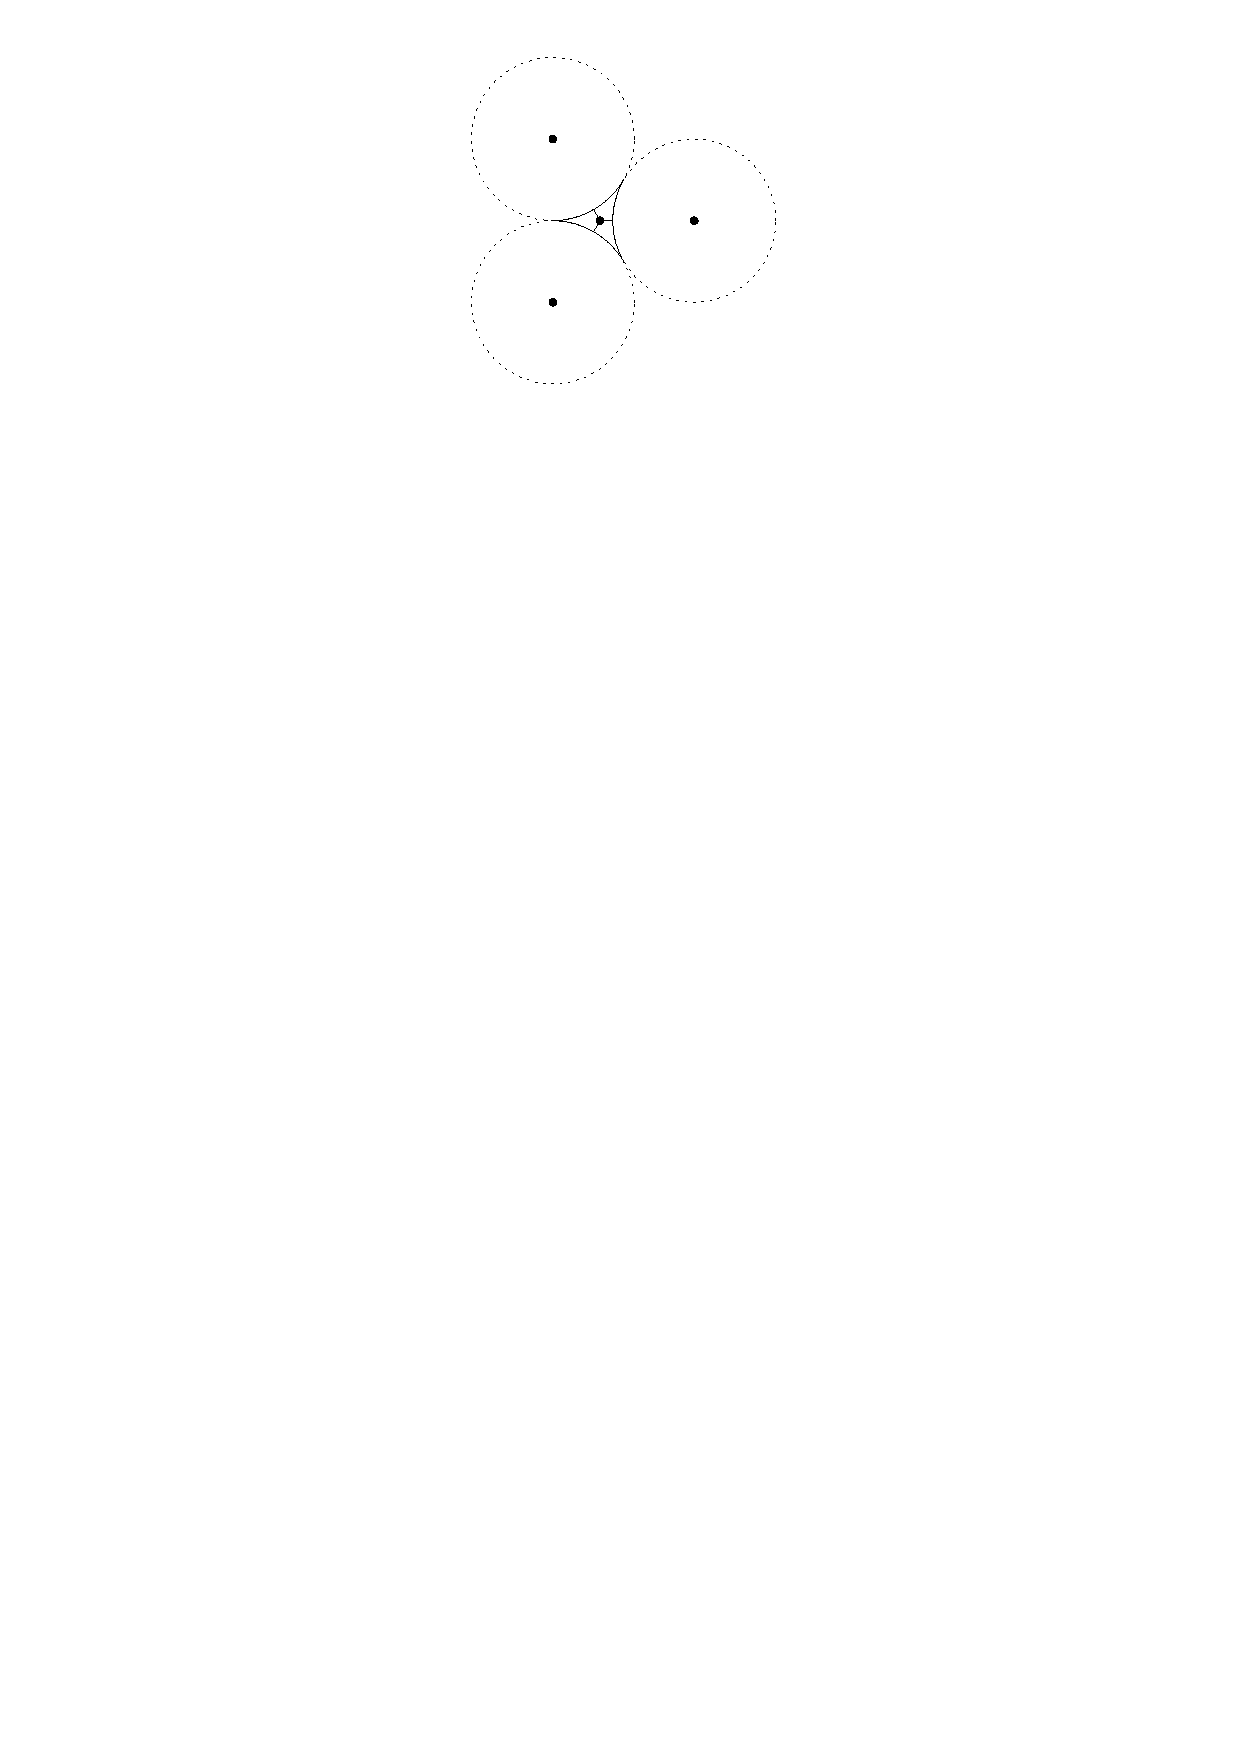
\includegraphics[width=.9\textwidth]{graphics/dhsi.pdf}
            \captionof{figure}{Caption Text}\label{gfx:dhsi.pdf}
            \end{center}
        \end{minipage}
    \end{columns}
\end{frame}
\begin{frame} \frametitle{DiskPackingReconfiguration.pdf}
    \begin{columns}[c]
    \column{.5\textwidth}
        \begin{itemize}
            \item[*] item 1
            \item[*] item 2
        \end{itemize}
    \column{.5\textwidth}
        \begin{minipage}{\linewidth}
            \begin{center}
            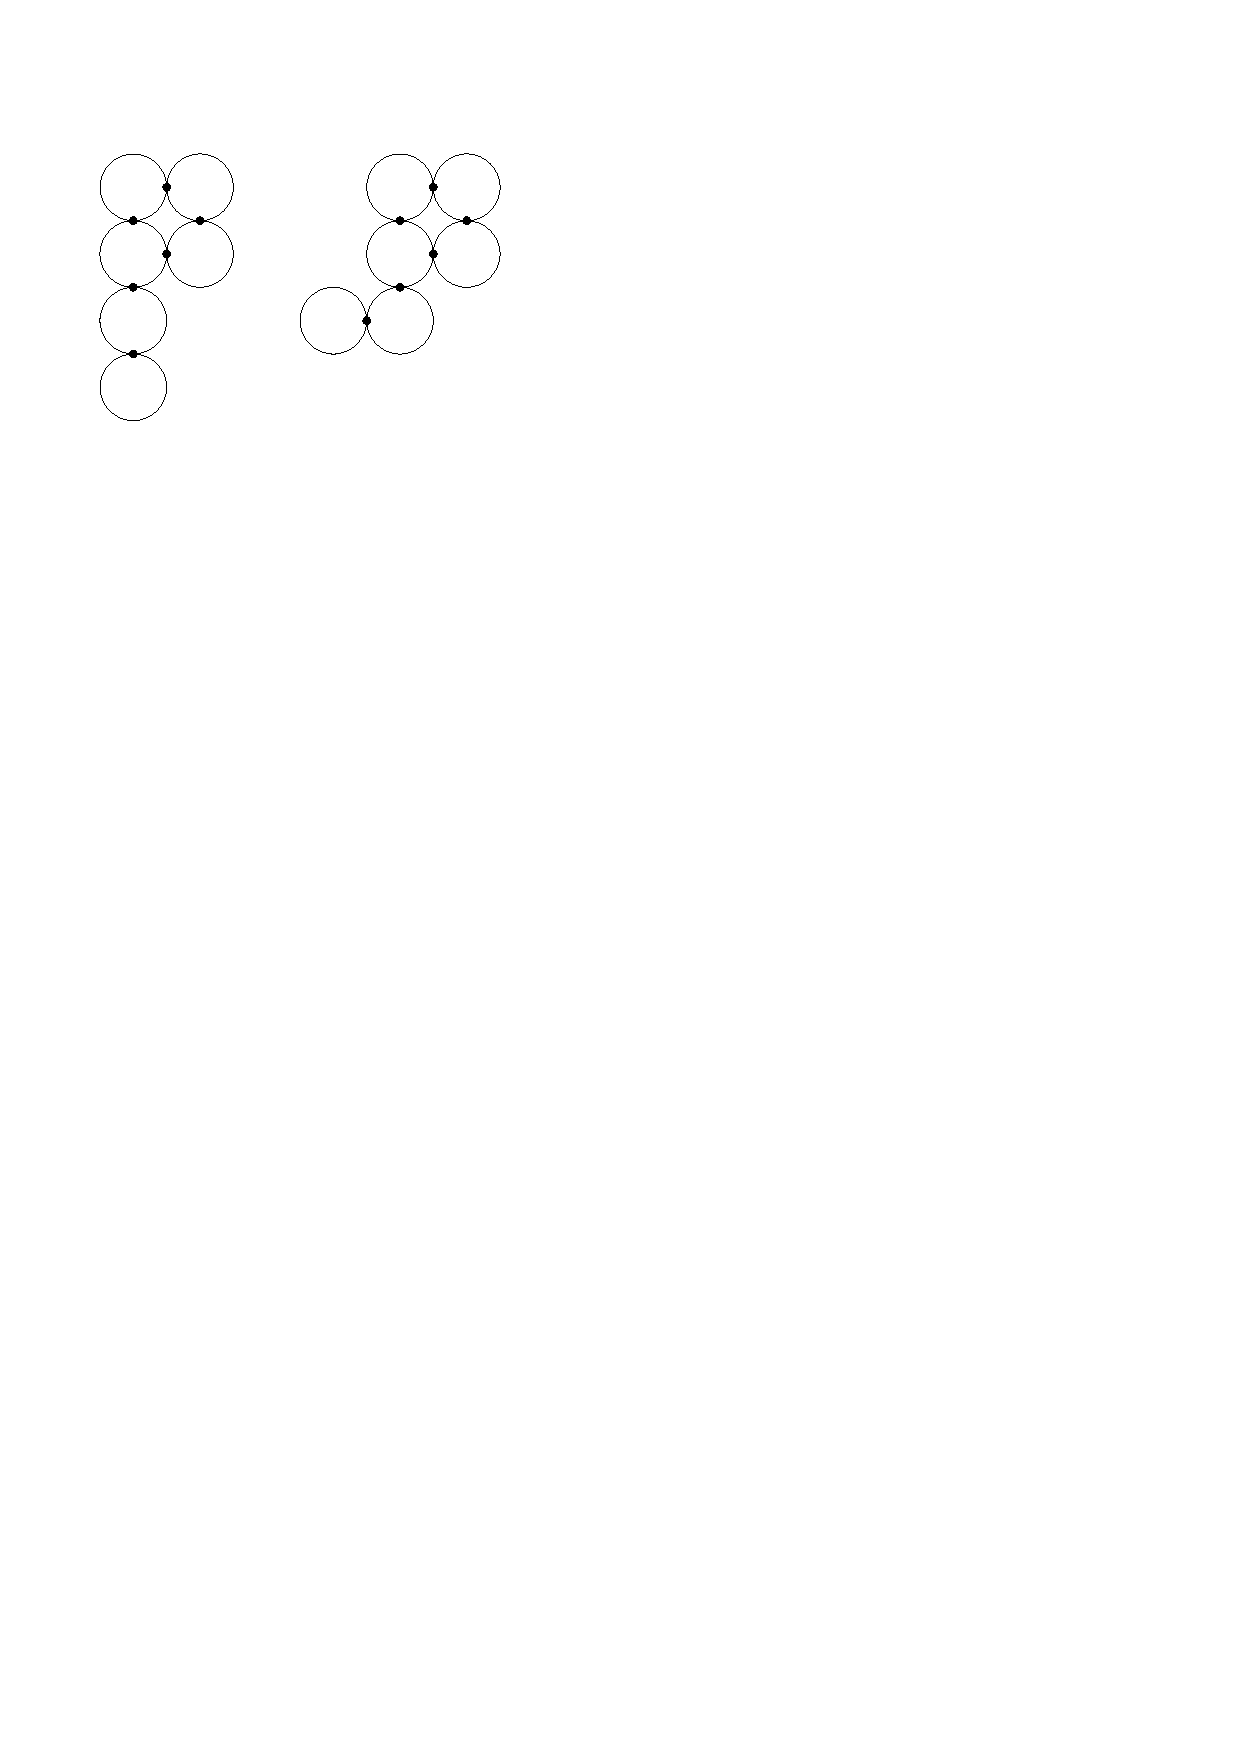
\includegraphics[width=.9\textwidth]{graphics/DiskPackingReconfiguration.pdf}
            \captionof{figure}{Caption Text}\label{gfx:DiskPackingReconfiguration.pdf}
            \end{center}
        \end{minipage}
    \end{columns}
\end{frame}
\begin{frame} \frametitle{diskPackingTheoremExample.pdf}
    \begin{columns}[c]
    \column{.5\textwidth}
        \begin{itemize}
            \item[*] item 1
            \item[*] item 2
        \end{itemize}
    \column{.5\textwidth}
        \begin{minipage}{\linewidth}
            \begin{center}
            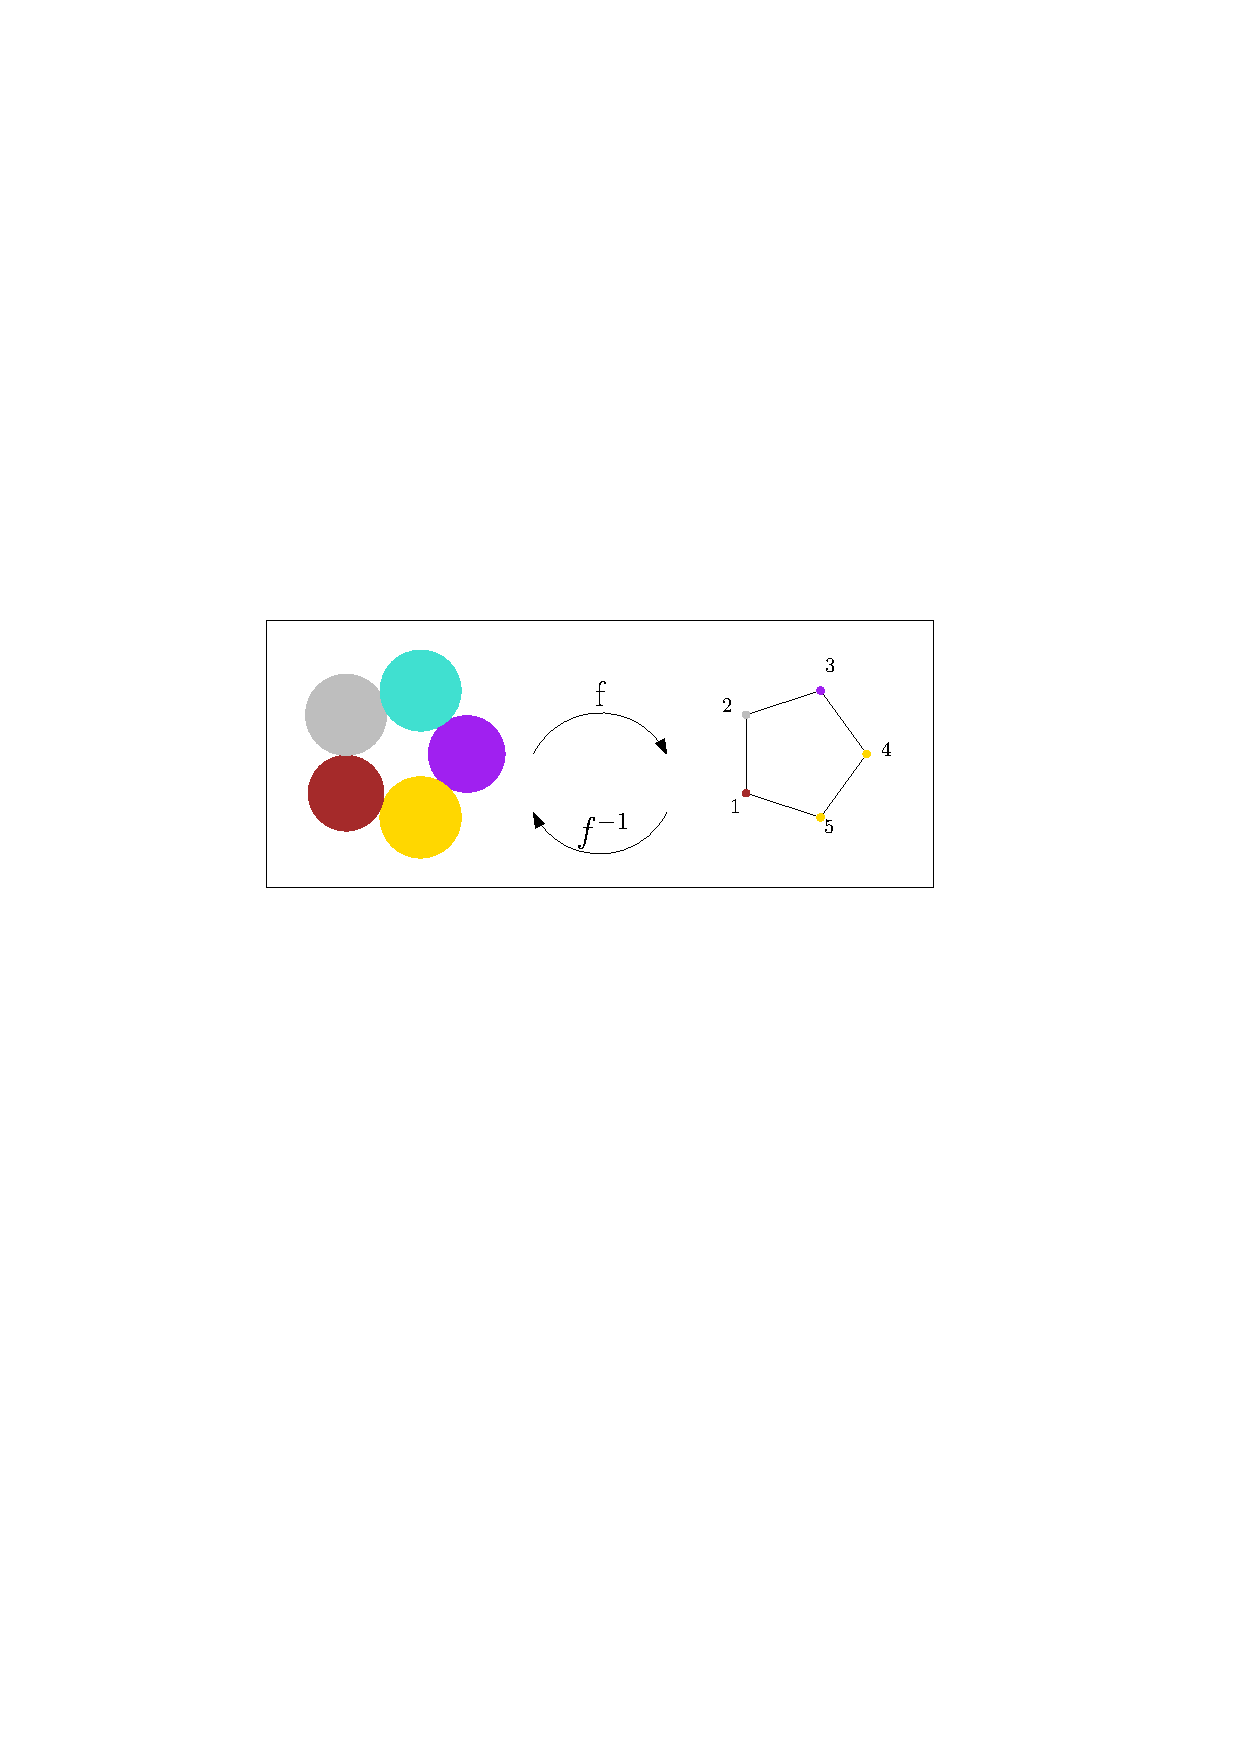
\includegraphics[width=.9\textwidth]{graphics/diskPackingTheoremExample.pdf}
            \captionof{figure}{Caption Text}\label{gfx:diskPackingTheoremExample.pdf}
            \end{center}
        \end{minipage}
    \end{columns}
\end{frame}
\begin{frame} \frametitle{dragonBallz.pdf}
    \begin{columns}[c]
    \column{.5\textwidth}
        \begin{itemize}
            \item[*] item 1
            \item[*] item 2
        \end{itemize}
    \column{.5\textwidth}
        \begin{minipage}{\linewidth}
            \begin{center}
            \includegraphics[width=.9\textwidth]{graphics/dragonBallz.pdf}
            \captionof{figure}{Caption Text}\label{gfx:dragonBallz.pdf}
            \end{center}
        \end{minipage}
    \end{columns}
\end{frame}
\begin{frame} \frametitle{dualBigHexagonalGrid.pdf}
    \begin{columns}[c]
    \column{.5\textwidth}
        \begin{itemize}
            \item[*] item 1
            \item[*] item 2
        \end{itemize}
    \column{.5\textwidth}
        \begin{minipage}{\linewidth}
            \begin{center}
            \includegraphics[width=.9\textwidth]{graphics/dualBigHexagonalGrid.pdf}
            \captionof{figure}{Caption Text}\label{gfx:dualBigHexagonalGrid.pdf}
            \end{center}
        \end{minipage}
    \end{columns}
\end{frame}
\begin{frame} \frametitle{dualSmallHexagonalGrid.pdf}
    \begin{columns}[c]
    \column{.5\textwidth}
        \begin{itemize}
            \item[*] item 1
            \item[*] item 2
        \end{itemize}
    \column{.5\textwidth}
        \begin{minipage}{\linewidth}
            \begin{center}
            \includegraphics[width=.9\textwidth]{graphics/dualSmallHexagonalGrid.pdf}
            \captionof{figure}{Caption Text}\label{gfx:dualSmallHexagonalGrid.pdf}
            \end{center}
        \end{minipage}
    \end{columns}
\end{frame}
\begin{frame} \frametitle{epsilonCenter.pdf}
    \begin{columns}[c]
    \column{.5\textwidth}
        \begin{itemize}
            \item[*] item 1
            \item[*] item 2
        \end{itemize}
    \column{.5\textwidth}
        \begin{minipage}{\linewidth}
            \begin{center}
            \includegraphics[width=.9\textwidth]{graphics/epsilonCenter.pdf}
            \captionof{figure}{Caption Text}\label{gfx:epsilonCenter.pdf}
            \end{center}
        \end{minipage}
    \end{columns}
\end{frame}
\begin{frame} \frametitle{epsilonCenterWithHexagon.pdf}
    \begin{columns}[c]
    \column{.5\textwidth}
        \begin{itemize}
            \item[*] item 1
            \item[*] item 2
        \end{itemize}
    \column{.5\textwidth}
        \begin{minipage}{\linewidth}
            \begin{center}
            \includegraphics[width=.9\textwidth]{graphics/epsilonCenterWithHexagon.pdf}
            \captionof{figure}{Caption Text}\label{gfx:epsilonCenterWithHexagon.pdf}
            \end{center}
        \end{minipage}
    \end{columns}
\end{frame}
\begin{frame} \frametitle{equivalentWheelEmbedding.pdf}
    \begin{columns}[c]
    \column{.5\textwidth}
        \begin{itemize}
            \item[*] item 1
            \item[*] item 2
        \end{itemize}
    \column{.5\textwidth}
        \begin{minipage}{\linewidth}
            \begin{center}
            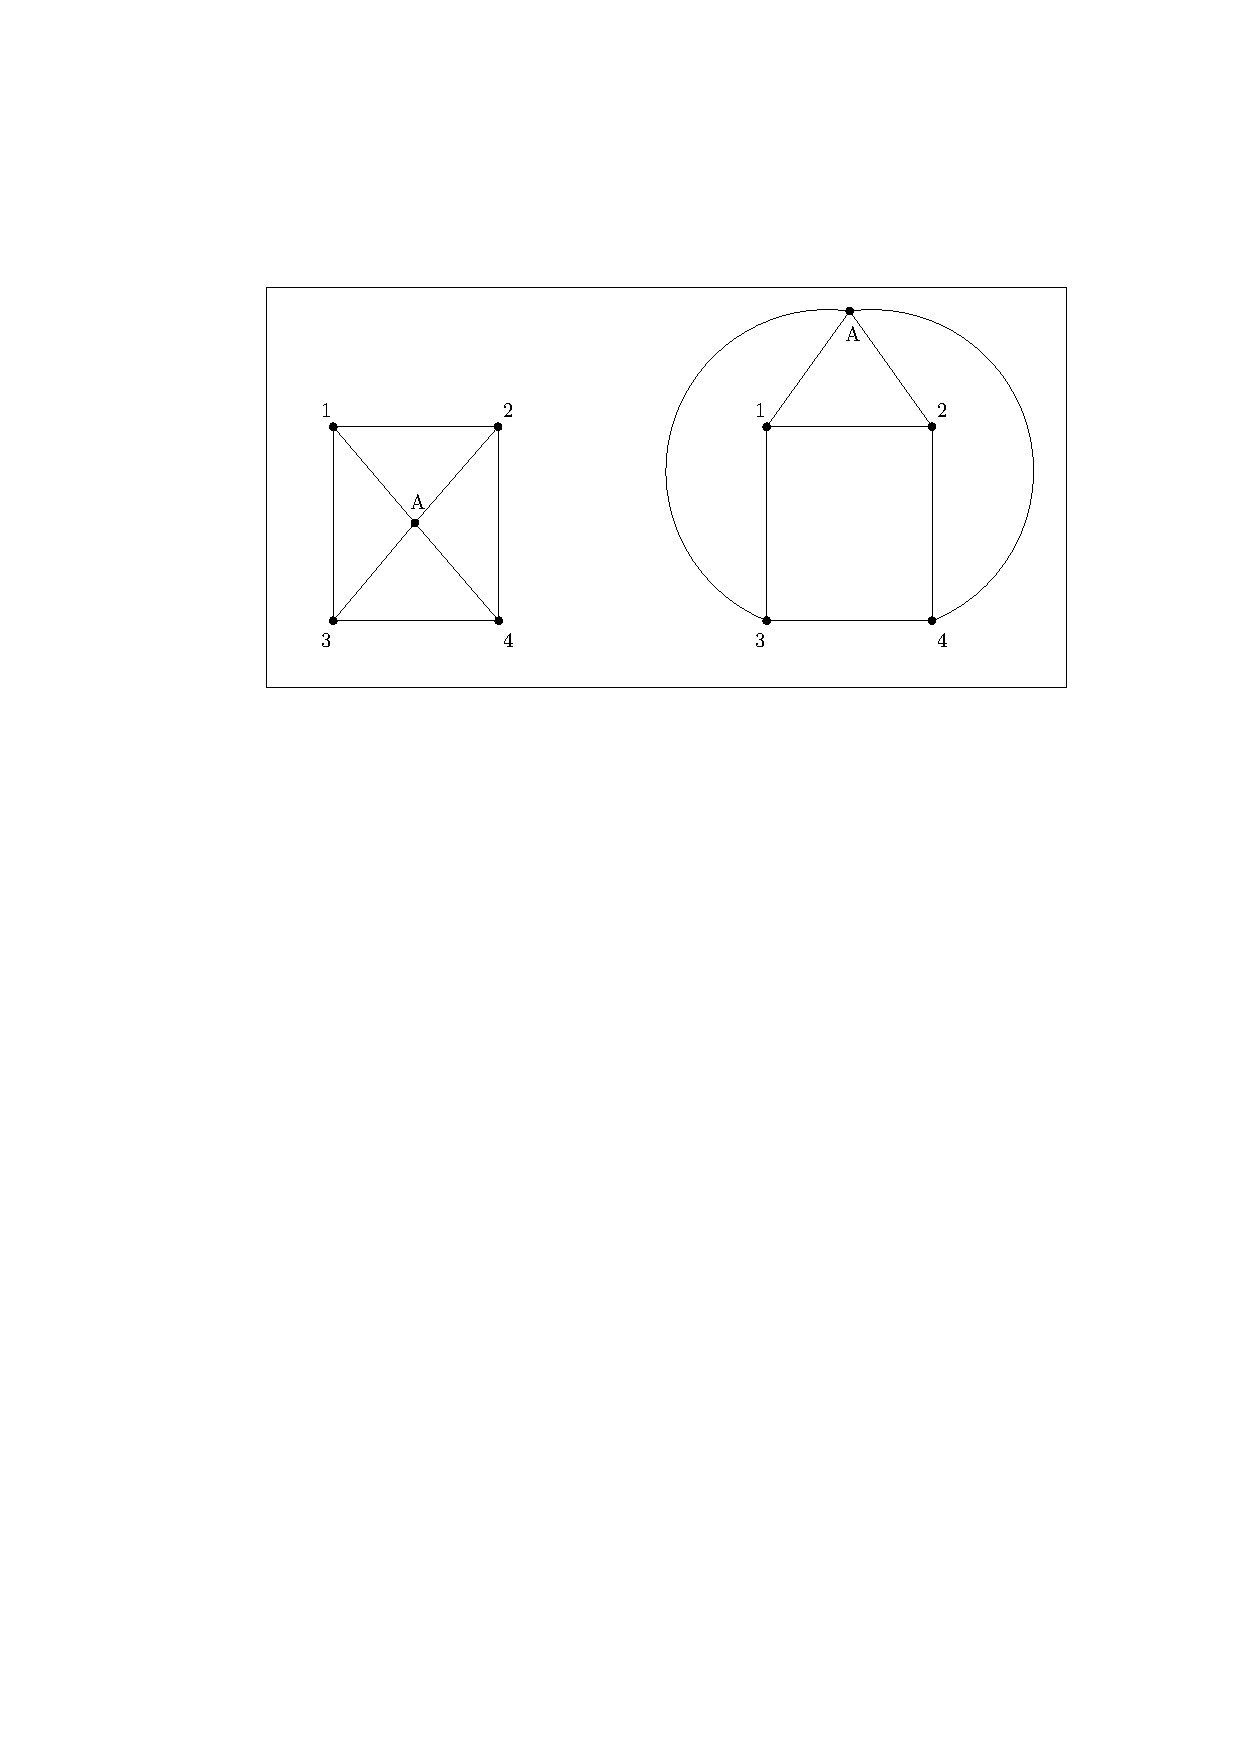
\includegraphics[width=.9\textwidth]{graphics/equivalentWheelEmbedding.pdf}
            \captionof{figure}{Caption Text}\label{gfx:equivalentWheelEmbedding.pdf}
            \end{center}
        \end{minipage}
    \end{columns}
\end{frame}
\begin{frame} \frametitle{FalseVariableNonNegatedLiteralTransmitter.pdf}
    \begin{columns}[c]
    \column{.5\textwidth}
        \begin{itemize}
            \item[*] item 1
            \item[*] item 2
        \end{itemize}
    \column{.5\textwidth}
        \begin{minipage}{\linewidth}
            \begin{center}
            \includegraphics[width=.9\textwidth]{graphics/FalseVariableNonNegatedLiteralTransmitter.pdf}
            \captionof{figure}{Caption Text}\label{gfx:FalseVariableNonNegatedLiteralTransmitter.pdf}
            \end{center}
        \end{minipage}
    \end{columns}
\end{frame}
\begin{frame} \frametitle{fig-assoc-hex.pdf}
    \begin{columns}[c]
    \column{.5\textwidth}
        \begin{itemize}
            \item[*] item 1
            \item[*] item 2
        \end{itemize}
    \column{.5\textwidth}
        \begin{minipage}{\linewidth}
            \begin{center}
            \includegraphics[width=.9\textwidth]{graphics/fig-assoc-hex.pdf}
            \captionof{figure}{Caption Text}\label{gfx:fig-assoc-hex.pdf}
            \end{center}
        \end{minipage}
    \end{columns}
\end{frame}
\begin{frame} \frametitle{fig-assoc.pdf}
    \begin{columns}[c]
    \column{.5\textwidth}
        \begin{itemize}
            \item[*] item 1
            \item[*] item 2
        \end{itemize}
    \column{.5\textwidth}
        \begin{minipage}{\linewidth}
            \begin{center}
            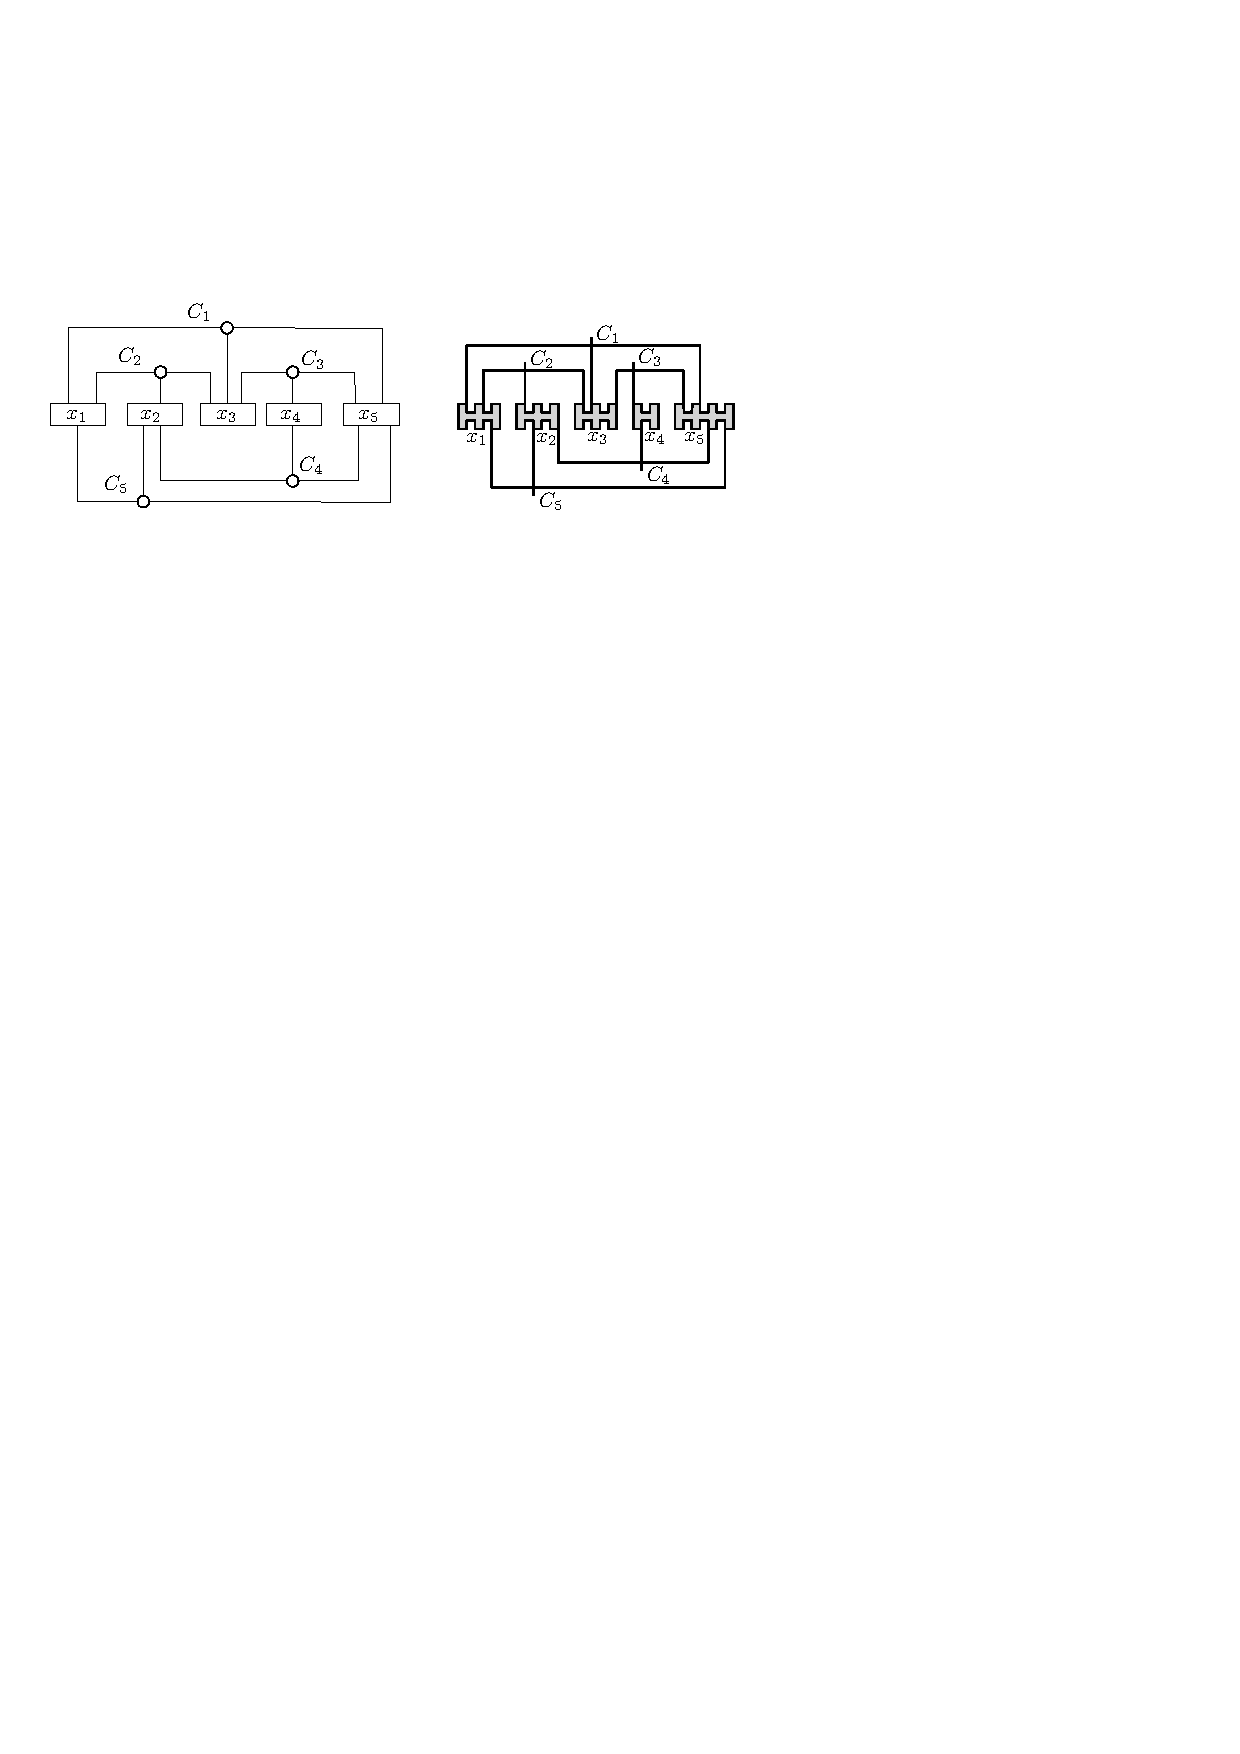
\includegraphics[width=.9\textwidth]{graphics/fig-assoc.pdf}
            \captionof{figure}{Caption Text}\label{gfx:fig-assoc.pdf}
            \end{center}
        \end{minipage}
    \end{columns}
\end{frame}
\begin{frame} \frametitle{fig-chains.pdf}
    \begin{columns}[c]
    \column{.5\textwidth}
        \begin{itemize}
            \item[*] item 1
            \item[*] item 2
        \end{itemize}
    \column{.5\textwidth}
        \begin{minipage}{\linewidth}
            \begin{center}
            \includegraphics[width=.9\textwidth]{graphics/fig-chains.pdf}
            \captionof{figure}{Caption Text}\label{gfx:fig-chains.pdf}
            \end{center}
        \end{minipage}
    \end{columns}
\end{frame}
\begin{frame} \frametitle{fig-clause-hex.pdf}
    \begin{columns}[c]
    \column{.5\textwidth}
        \begin{itemize}
            \item[*] item 1
            \item[*] item 2
        \end{itemize}
    \column{.5\textwidth}
        \begin{minipage}{\linewidth}
            \begin{center}
            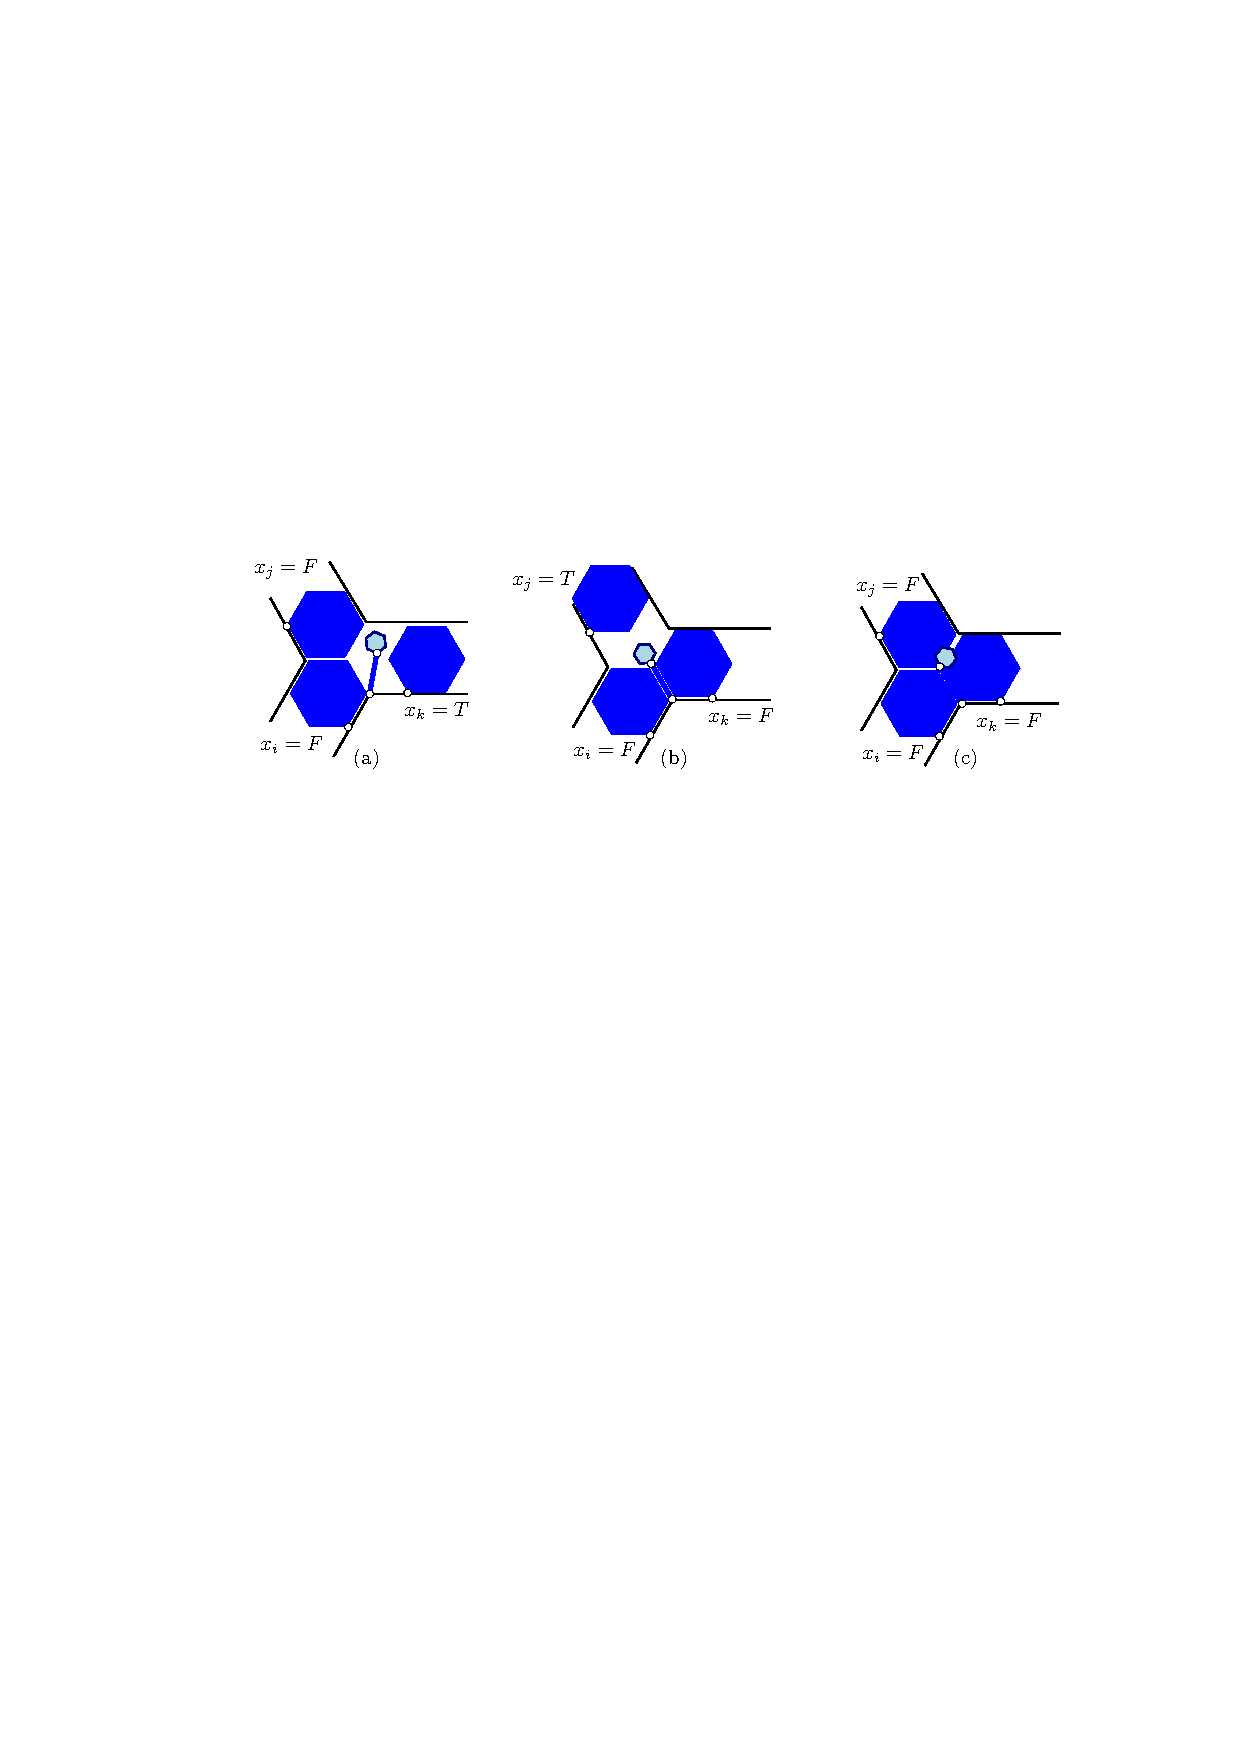
\includegraphics[width=.9\textwidth]{graphics/fig-clause-hex.pdf}
            \captionof{figure}{Caption Text}\label{gfx:fig-clause-hex.pdf}
            \end{center}
        \end{minipage}
    \end{columns}
\end{frame}
\begin{frame} \frametitle{fig-clause.pdf}
    \begin{columns}[c]
    \column{.5\textwidth}
        \begin{itemize}
            \item[*] item 1
            \item[*] item 2
        \end{itemize}
    \column{.5\textwidth}
        \begin{minipage}{\linewidth}
            \begin{center}
            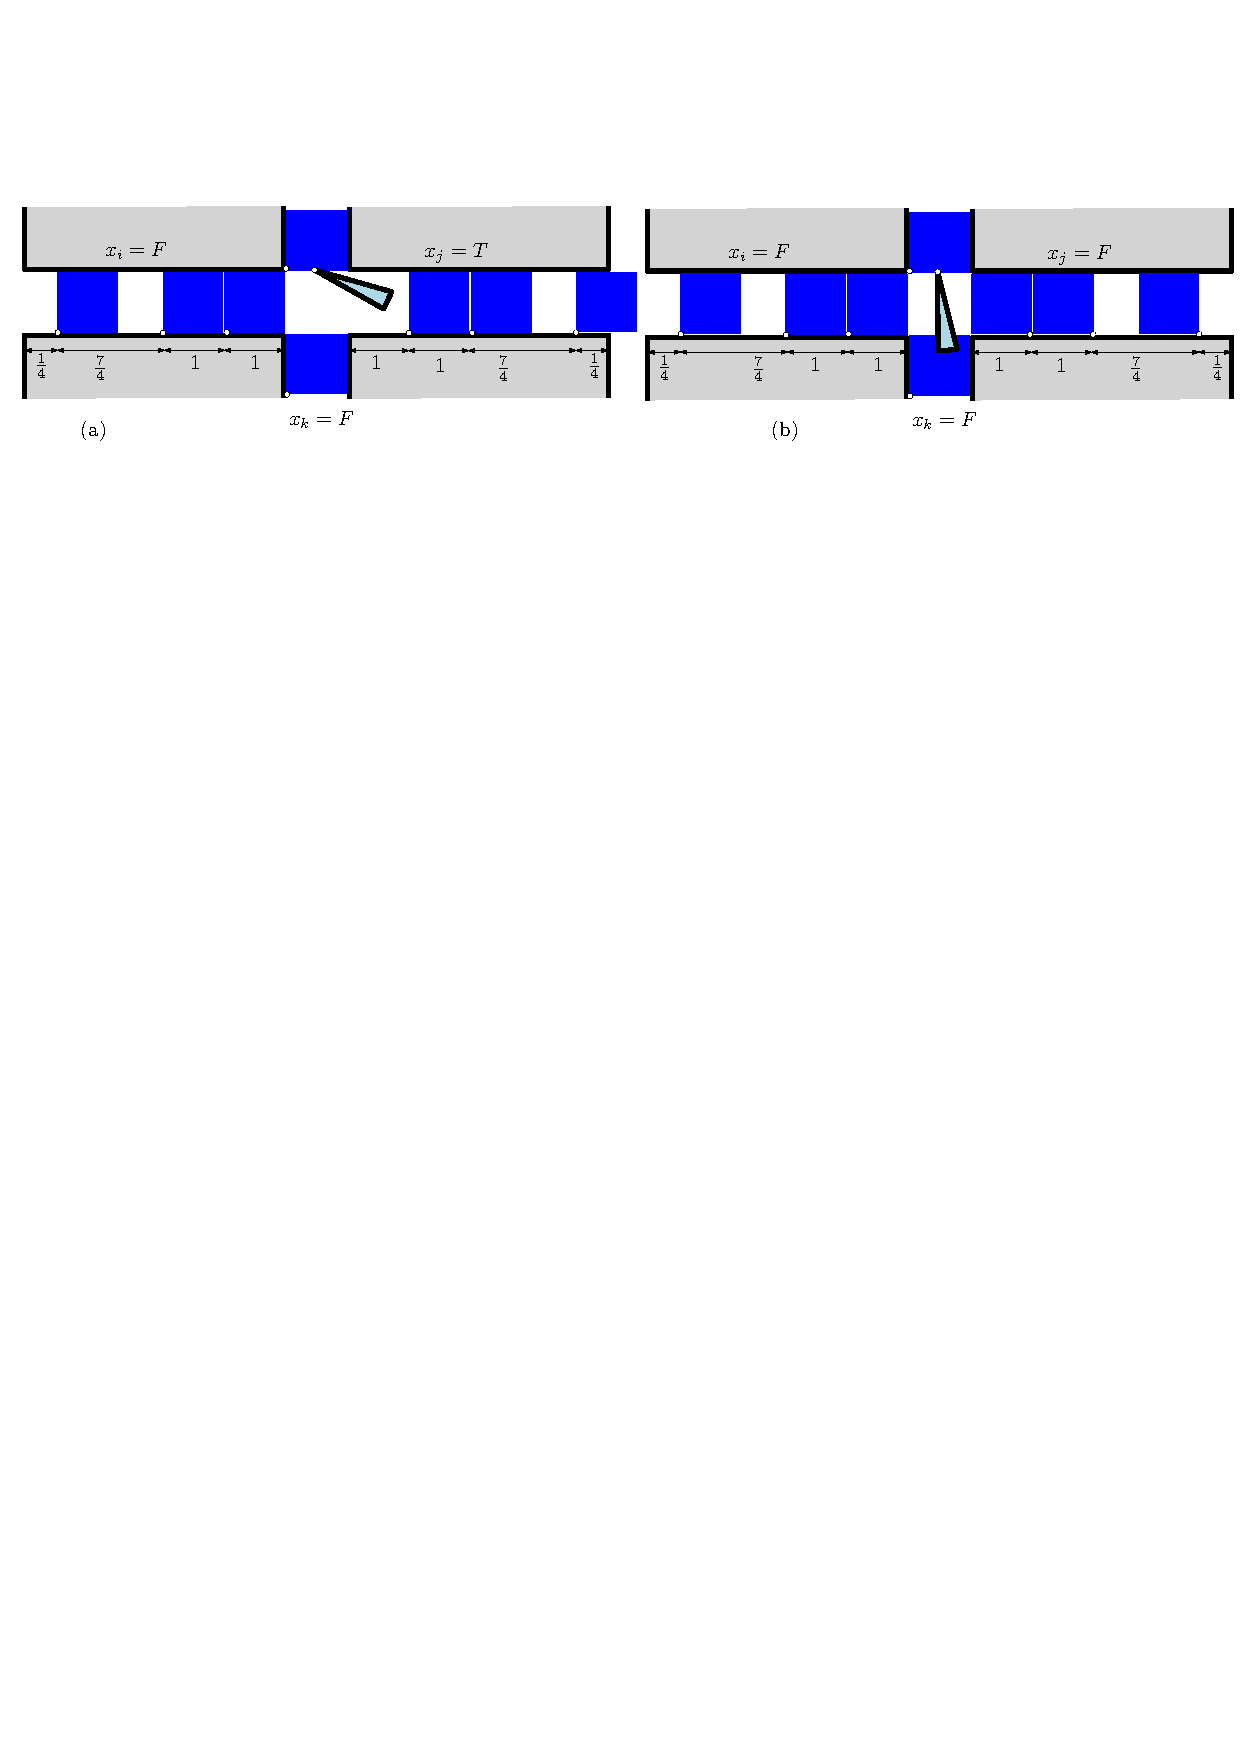
\includegraphics[width=.9\textwidth]{graphics/fig-clause.pdf}
            \captionof{figure}{Caption Text}\label{gfx:fig-clause.pdf}
            \end{center}
        \end{minipage}
    \end{columns}
\end{frame}
\begin{frame} \frametitle{fig-frame-hex.pdf}
    \begin{columns}[c]
    \column{.5\textwidth}
        \begin{itemize}
            \item[*] item 1
            \item[*] item 2
        \end{itemize}
    \column{.5\textwidth}
        \begin{minipage}{\linewidth}
            \begin{center}
            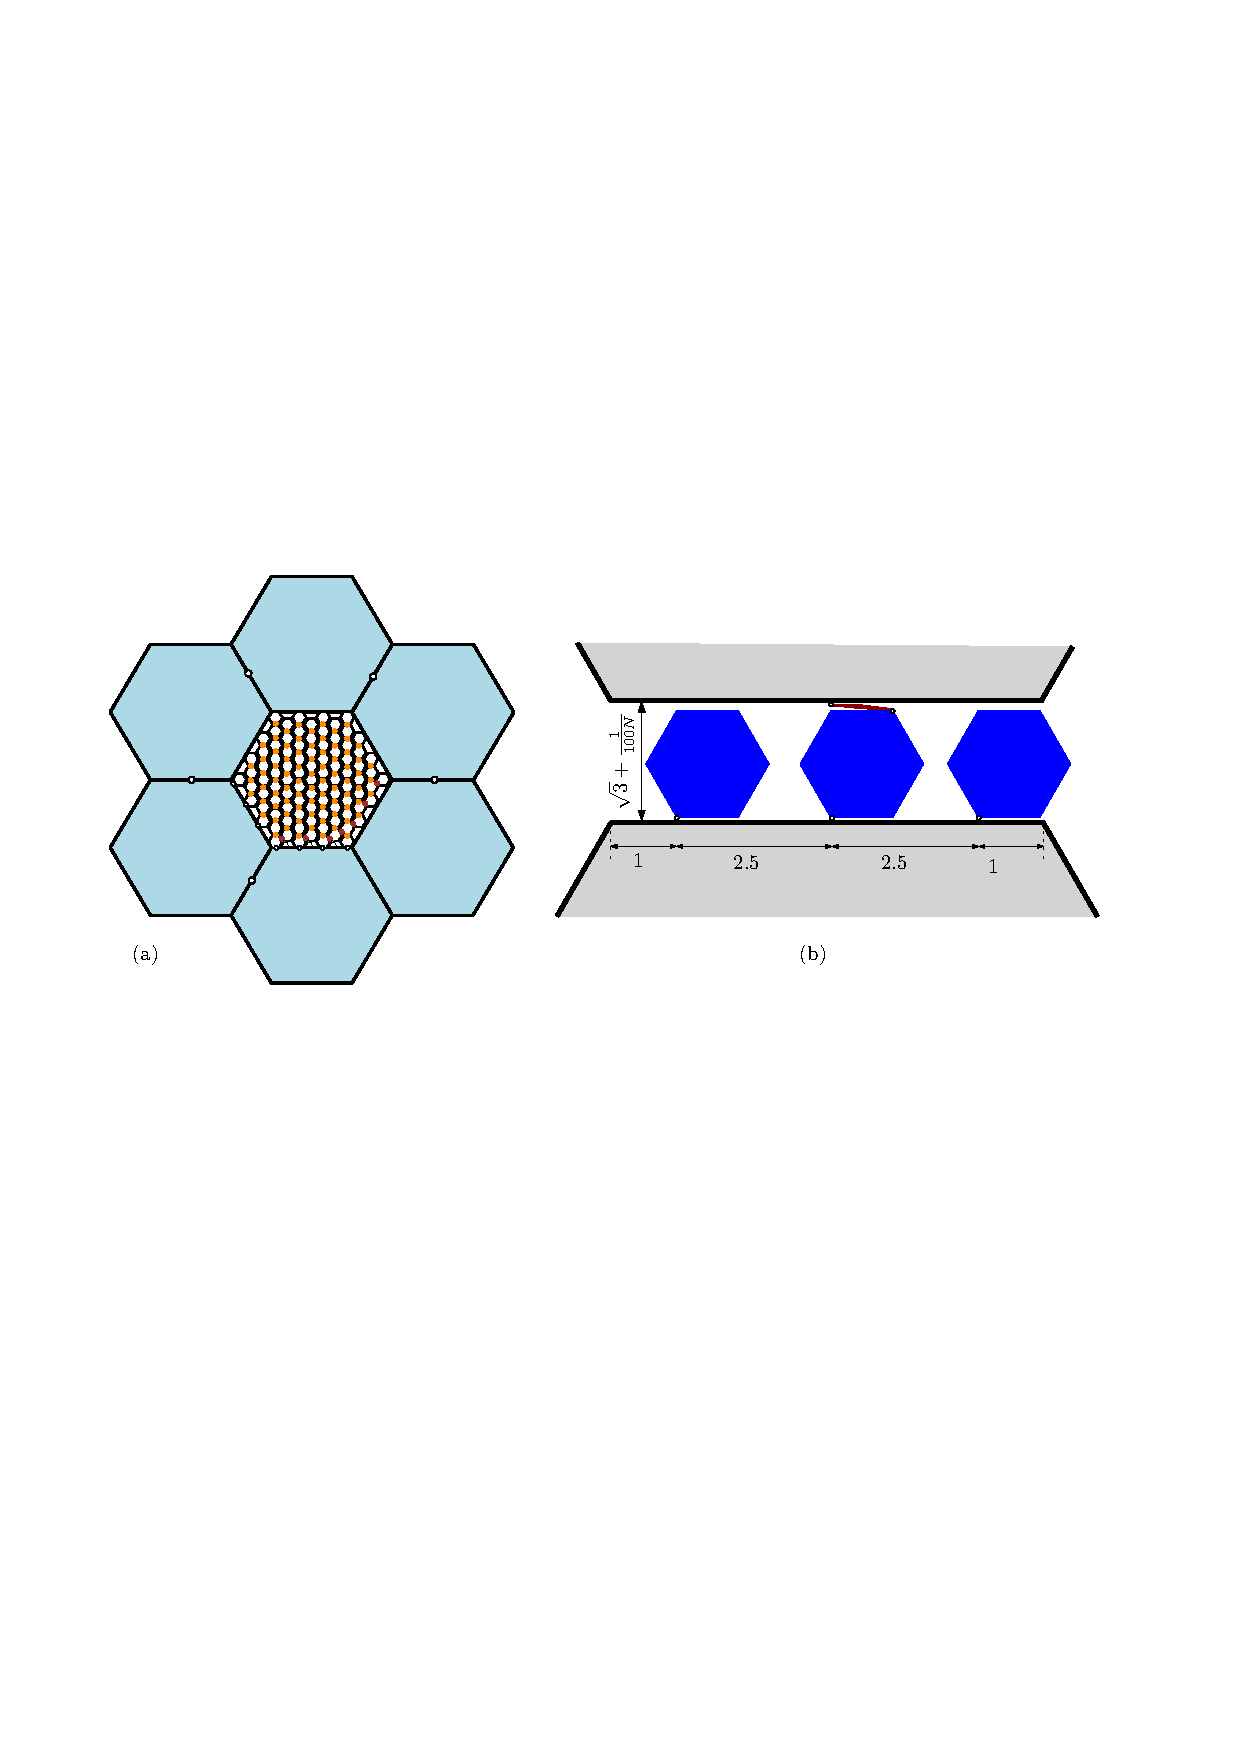
\includegraphics[width=.9\textwidth]{graphics/fig-frame-hex.pdf}
            \captionof{figure}{Caption Text}\label{gfx:fig-frame-hex.pdf}
            \end{center}
        \end{minipage}
    \end{columns}
\end{frame}
\begin{frame} \frametitle{fig-frame.pdf}
    \begin{columns}[c]
    \column{.5\textwidth}
        \begin{itemize}
            \item[*] item 1
            \item[*] item 2
        \end{itemize}
    \column{.5\textwidth}
        \begin{minipage}{\linewidth}
            \begin{center}
            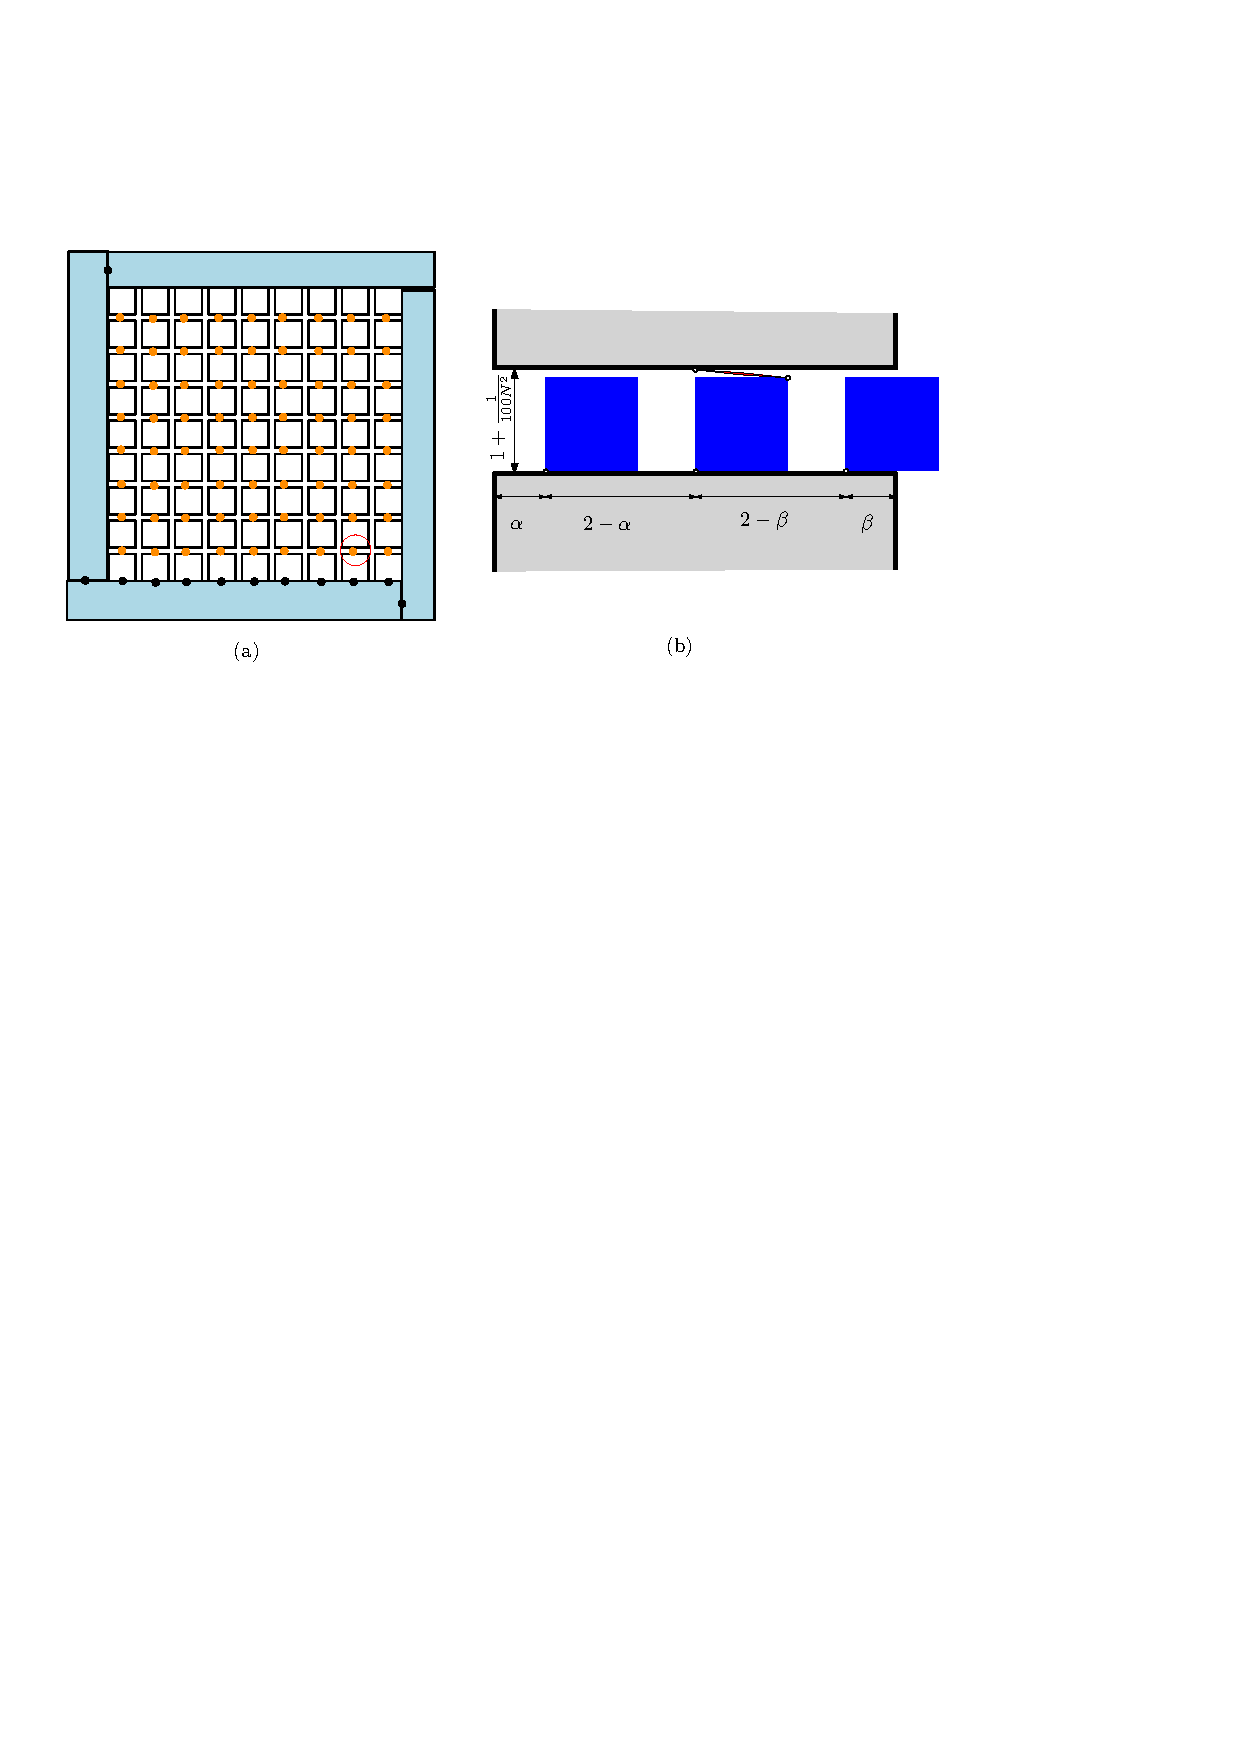
\includegraphics[width=.9\textwidth]{graphics/fig-frame.pdf}
            \captionof{figure}{Caption Text}\label{gfx:fig-frame.pdf}
            \end{center}
        \end{minipage}
    \end{columns}
\end{frame}
\begin{frame} \frametitle{fig-hexagon.pdf}
    \begin{columns}[c]
    \column{.5\textwidth}
        \begin{itemize}
            \item[*] item 1
            \item[*] item 2
        \end{itemize}
    \column{.5\textwidth}
        \begin{minipage}{\linewidth}
            \begin{center}
            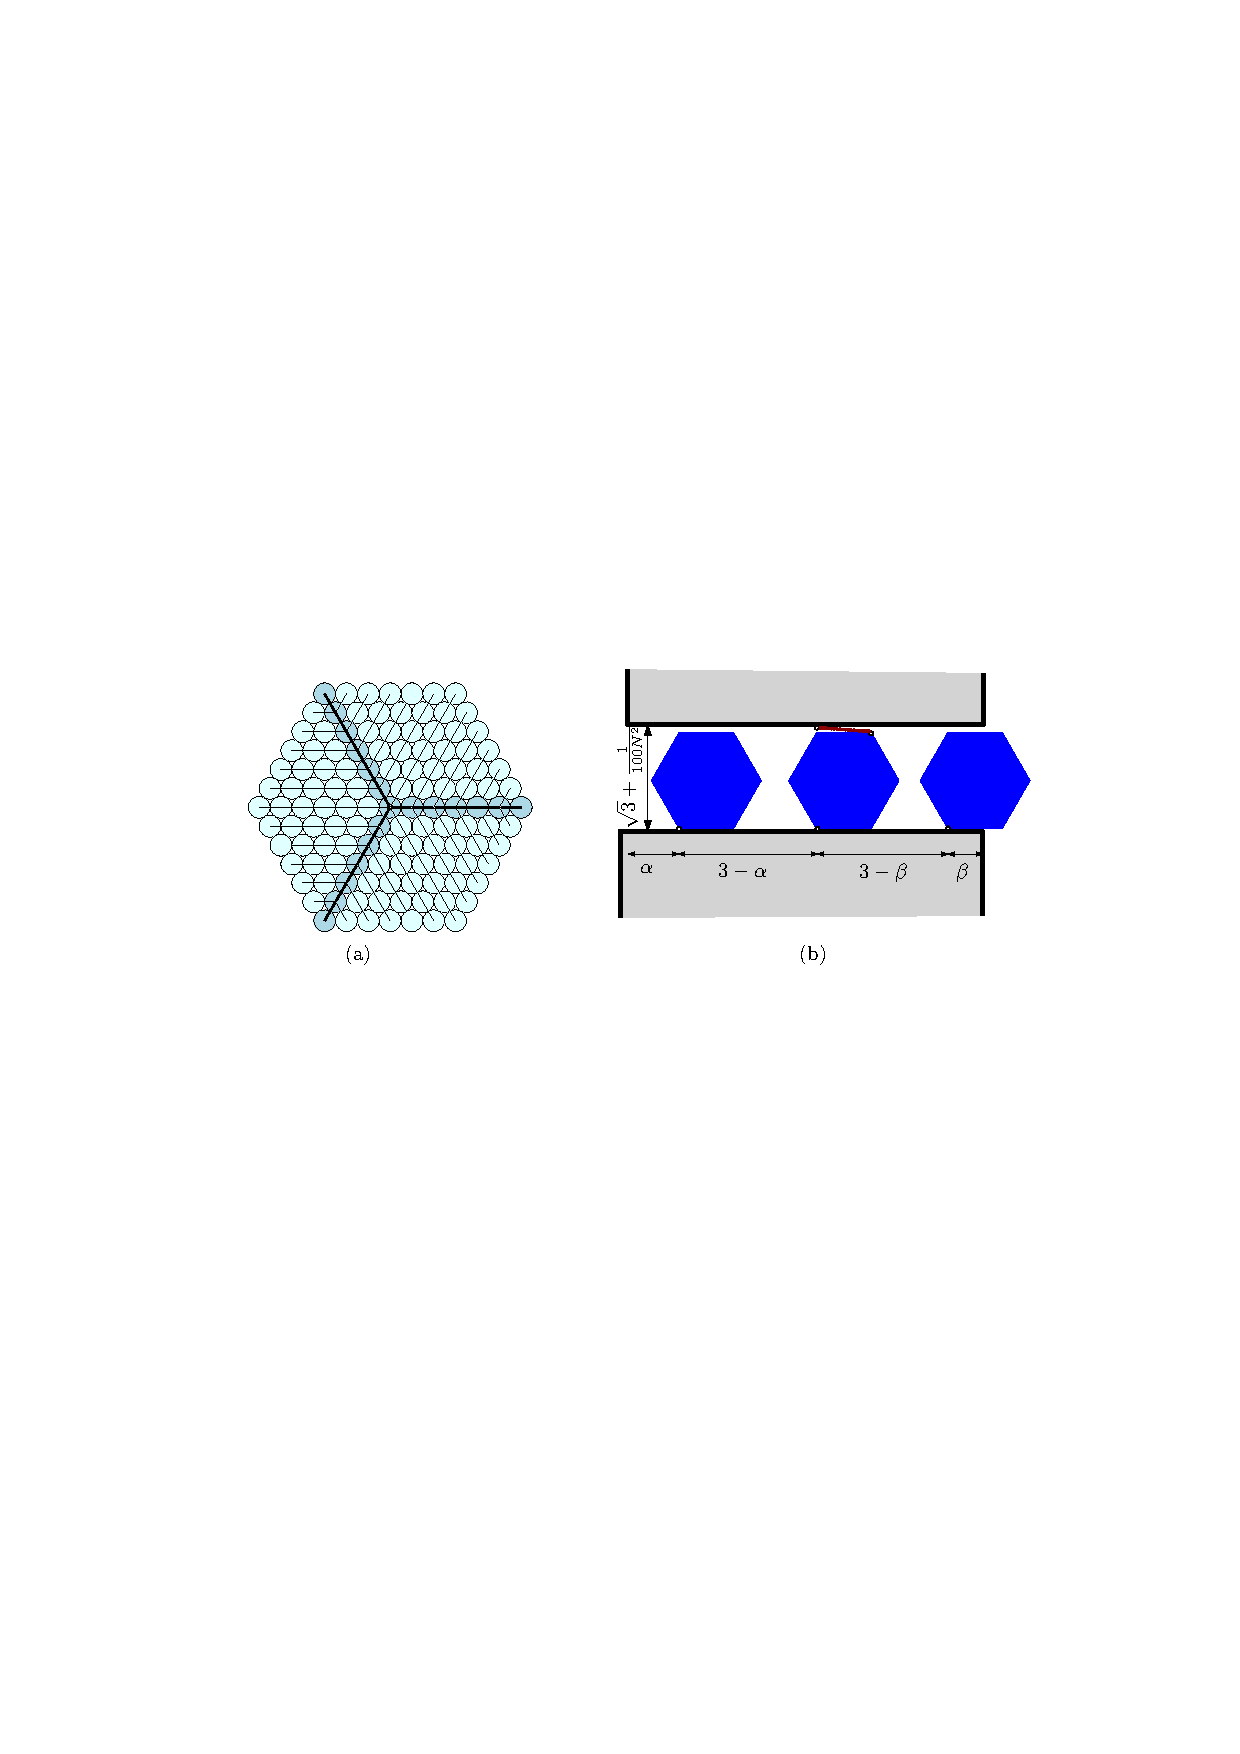
\includegraphics[width=.9\textwidth]{graphics/fig-hexagon.pdf}
            \captionof{figure}{Caption Text}\label{gfx:fig-hexagon.pdf}
            \end{center}
        \end{minipage}
    \end{columns}
\end{frame}
\begin{frame} \frametitle{fig-logic.pdf}
    \begin{columns}[c]
    \column{.5\textwidth}
        \begin{itemize}
            \item[*] item 1
            \item[*] item 2
        \end{itemize}
    \column{.5\textwidth}
        \begin{minipage}{\linewidth}
            \begin{center}
            \includegraphics[width=.9\textwidth]{graphics/fig-logic.pdf}
            \captionof{figure}{Caption Text}\label{gfx:fig-logic.pdf}
            \end{center}
        \end{minipage}
    \end{columns}
\end{frame}
\begin{frame} \frametitle{fig-transmitter-hex copy.pdf}
    \begin{columns}[c]
    \column{.5\textwidth}
        \begin{itemize}
            \item[*] item 1
            \item[*] item 2
        \end{itemize}
    \column{.5\textwidth}
        \begin{minipage}{\linewidth}
            \begin{center}
            \includegraphics[width=.9\textwidth]{graphics/fig-transmitter-hex copy.pdf}
            \captionof{figure}{Caption Text}\label{gfx:fig-transmitter-hex copy.pdf}
            \end{center}
        \end{minipage}
    \end{columns}
\end{frame}
\begin{frame} \frametitle{fig-transmitter-hex.pdf}
    \begin{columns}[c]
    \column{.5\textwidth}
        \begin{itemize}
            \item[*] item 1
            \item[*] item 2
        \end{itemize}
    \column{.5\textwidth}
        \begin{minipage}{\linewidth}
            \begin{center}
            \includegraphics[width=.9\textwidth]{graphics/fig-transmitter-hex.pdf}
            \captionof{figure}{Caption Text}\label{gfx:fig-transmitter-hex.pdf}
            \end{center}
        \end{minipage}
    \end{columns}
\end{frame}
\begin{frame} \frametitle{fig-transmitter.pdf}
    \begin{columns}[c]
    \column{.5\textwidth}
        \begin{itemize}
            \item[*] item 1
            \item[*] item 2
        \end{itemize}
    \column{.5\textwidth}
        \begin{minipage}{\linewidth}
            \begin{center}
            \includegraphics[width=.9\textwidth]{graphics/fig-transmitter.pdf}
            \captionof{figure}{Caption Text}\label{gfx:fig-transmitter.pdf}
            \end{center}
        \end{minipage}
    \end{columns}
\end{frame}
\begin{frame} \frametitle{fig-triangles.pdf}
    \begin{columns}[c]
    \column{.5\textwidth}
        \begin{itemize}
            \item[*] item 1
            \item[*] item 2
        \end{itemize}
    \column{.5\textwidth}
        \begin{minipage}{\linewidth}
            \begin{center}
            \includegraphics[width=.9\textwidth]{graphics/fig-triangles.pdf}
            \captionof{figure}{Caption Text}\label{gfx:fig-triangles.pdf}
            \end{center}
        \end{minipage}
    \end{columns}
\end{frame}
\begin{frame} \frametitle{fig-ushape.pdf}
    \begin{columns}[c]
    \column{.5\textwidth}
        \begin{itemize}
            \item[*] item 1
            \item[*] item 2
        \end{itemize}
    \column{.5\textwidth}
        \begin{minipage}{\linewidth}
            \begin{center}
            \includegraphics[width=.9\textwidth]{graphics/fig-ushape.pdf}
            \captionof{figure}{Caption Text}\label{gfx:fig-ushape.pdf}
            \end{center}
        \end{minipage}
    \end{columns}
\end{frame}
\begin{frame} \frametitle{fig-variable-hex+.pdf}
    \begin{columns}[c]
    \column{.5\textwidth}
        \begin{itemize}
            \item[*] item 1
            \item[*] item 2
        \end{itemize}
    \column{.5\textwidth}
        \begin{minipage}{\linewidth}
            \begin{center}
            \includegraphics[width=.9\textwidth]{graphics/fig-variable-hex+.pdf}
            \captionof{figure}{Caption Text}\label{gfx:fig-variable-hex+.pdf}
            \end{center}
        \end{minipage}
    \end{columns}
\end{frame}
\begin{frame} \frametitle{fig-variable.pdf}
    \begin{columns}[c]
    \column{.5\textwidth}
        \begin{itemize}
            \item[*] item 1
            \item[*] item 2
        \end{itemize}
    \column{.5\textwidth}
        \begin{minipage}{\linewidth}
            \begin{center}
            \includegraphics[width=.9\textwidth]{graphics/fig-variable.pdf}
            \captionof{figure}{Caption Text}\label{gfx:fig-variable.pdf}
            \end{center}
        \end{minipage}
    \end{columns}
\end{frame}
\begin{frame} \frametitle{fig1+.pdf}
    \begin{columns}[c]
    \column{.5\textwidth}
        \begin{itemize}
            \item[*] item 1
            \item[*] item 2
        \end{itemize}
    \column{.5\textwidth}
        \begin{minipage}{\linewidth}
            \begin{center}
            \includegraphics[width=.9\textwidth]{graphics/fig1+.pdf}
            \captionof{figure}{Caption Text}\label{gfx:fig1+.pdf}
            \end{center}
        \end{minipage}
    \end{columns}
\end{frame}
\begin{frame} \frametitle{fig1.pdf}
    \begin{columns}[c]
    \column{.5\textwidth}
        \begin{itemize}
            \item[*] item 1
            \item[*] item 2
        \end{itemize}
    \column{.5\textwidth}
        \begin{minipage}{\linewidth}
            \begin{center}
            \includegraphics[width=.9\textwidth]{graphics/fig1.pdf}
            \captionof{figure}{Caption Text}\label{gfx:fig1.pdf}
            \end{center}
        \end{minipage}
    \end{columns}
\end{frame}
\begin{frame} \frametitle{FlagWithRhombus.pdf}
    \begin{columns}[c]
    \column{.5\textwidth}
        \begin{itemize}
            \item[*] item 1
            \item[*] item 2
        \end{itemize}
    \column{.5\textwidth}
        \begin{minipage}{\linewidth}
            \begin{center}
            \includegraphics[width=.9\textwidth]{graphics/FlagWithRhombus.pdf}
            \captionof{figure}{Caption Text}\label{gfx:FlagWithRhombus.pdf}
            \end{center}
        \end{minipage}
    \end{columns}
\end{frame}
\begin{frame} \frametitle{FlexibleHexagons.pdf}
    \begin{columns}[c]
    \column{.5\textwidth}
        \begin{itemize}
            \item[*] item 1
            \item[*] item 2
        \end{itemize}
    \column{.5\textwidth}
        \begin{minipage}{\linewidth}
            \begin{center}
            \includegraphics[width=.9\textwidth]{graphics/FlexibleHexagons.pdf}
            \captionof{figure}{Caption Text}\label{gfx:FlexibleHexagons.pdf}
            \end{center}
        \end{minipage}
    \end{columns}
\end{frame}
\begin{frame} \frametitle{FrameObstacleHexagonCloseUp.pdf}
    \begin{columns}[c]
    \column{.5\textwidth}
        \begin{itemize}
            \item[*] item 1
            \item[*] item 2
        \end{itemize}
    \column{.5\textwidth}
        \begin{minipage}{\linewidth}
            \begin{center}
            \includegraphics[width=.9\textwidth]{graphics/FrameObstacleHexagonCloseUp.pdf}
            \captionof{figure}{Caption Text}\label{gfx:FrameObstacleHexagonCloseUp.pdf}
            \end{center}
        \end{minipage}
    \end{columns}
\end{frame}
\begin{frame} \frametitle{freeJointPinnedJoint.pdf}
    \begin{columns}[c]
    \column{.5\textwidth}
        \begin{itemize}
            \item[*] item 1
            \item[*] item 2
        \end{itemize}
    \column{.5\textwidth}
        \begin{minipage}{\linewidth}
            \begin{center}
            \includegraphics[width=.9\textwidth]{graphics/freeJointPinnedJoint.pdf}
            \captionof{figure}{Caption Text}\label{gfx:freeJointPinnedJoint.pdf}
            \end{center}
        \end{minipage}
    \end{columns}
\end{frame}
\begin{frame} \frametitle{GeometricDissectionBusschop.pdf}
    \begin{columns}[c]
    \column{.5\textwidth}
        \begin{itemize}
            \item[*] item 1
            \item[*] item 2
        \end{itemize}
    \column{.5\textwidth}
        \begin{minipage}{\linewidth}
            \begin{center}
            \includegraphics[width=.9\textwidth]{graphics/GeometricDissectionBusschop.pdf}
            \captionof{figure}{Caption Text}\label{gfx:GeometricDissectionBusschop.pdf}
            \end{center}
        \end{minipage}
    \end{columns}
\end{frame}
\begin{frame} \frametitle{graphIsomorphismExample.pdf}
    \begin{columns}[c]
    \column{.5\textwidth}
        \begin{itemize}
            \item[*] item 1
            \item[*] item 2
        \end{itemize}
    \column{.5\textwidth}
        \begin{minipage}{\linewidth}
            \begin{center}
            \includegraphics[width=.9\textwidth]{graphics/graphIsomorphismExample.pdf}
            \captionof{figure}{Caption Text}\label{gfx:graphIsomorphismExample.pdf}
            \end{center}
        \end{minipage}
    \end{columns}
\end{frame}
\begin{frame} \frametitle{HaberdasherProblem.pdf}
    \begin{columns}[c]
    \column{.5\textwidth}
        \begin{itemize}
            \item[*] item 1
            \item[*] item 2
        \end{itemize}
    \column{.5\textwidth}
        \begin{minipage}{\linewidth}
            \begin{center}
            \includegraphics[width=.9\textwidth]{graphics/HaberdasherProblem.pdf}
            \captionof{figure}{Caption Text}\label{gfx:HaberdasherProblem.pdf}
            \end{center}
        \end{minipage}
    \end{columns}
\end{frame}
\begin{frame} \frametitle{HalfSizeHexagon.pdf}
    \begin{columns}[c]
    \column{.5\textwidth}
        \begin{itemize}
            \item[*] item 1
            \item[*] item 2
        \end{itemize}
    \column{.5\textwidth}
        \begin{minipage}{\linewidth}
            \begin{center}
            \includegraphics[width=.9\textwidth]{graphics/HalfSizeHexagon.pdf}
            \captionof{figure}{Caption Text}\label{gfx:HalfSizeHexagon.pdf}
            \end{center}
        \end{minipage}
    \end{columns}
\end{frame}
\begin{frame} \frametitle{HausdorffDistanceExample1.pdf}
    \begin{columns}[c]
    \column{.5\textwidth}
        \begin{itemize}
            \item[*] item 1
            \item[*] item 2
        \end{itemize}
    \column{.5\textwidth}
        \begin{minipage}{\linewidth}
            \begin{center}
            \includegraphics[width=.9\textwidth]{graphics/HausdorffDistanceExample1.pdf}
            \captionof{figure}{Caption Text}\label{gfx:HausdorffDistanceExample1.pdf}
            \end{center}
        \end{minipage}
    \end{columns}
\end{frame}
\begin{frame} \frametitle{HausdorffDistanceExample1Small.pdf}
    \begin{columns}[c]
    \column{.5\textwidth}
        \begin{itemize}
            \item[*] item 1
            \item[*] item 2
        \end{itemize}
    \column{.5\textwidth}
        \begin{minipage}{\linewidth}
            \begin{center}
            \includegraphics[width=.9\textwidth]{graphics/HausdorffDistanceExample1Small.pdf}
            \captionof{figure}{Caption Text}\label{gfx:HausdorffDistanceExample1Small.pdf}
            \end{center}
        \end{minipage}
    \end{columns}
\end{frame}
\begin{frame} \frametitle{hexagonalConstructionOfJSmall.pdf}
    \begin{columns}[c]
    \column{.5\textwidth}
        \begin{itemize}
            \item[*] item 1
            \item[*] item 2
        \end{itemize}
    \column{.5\textwidth}
        \begin{minipage}{\linewidth}
            \begin{center}
            \includegraphics[width=.9\textwidth]{graphics/hexagonalConstructionOfJSmall.pdf}
            \captionof{figure}{Caption Text}\label{gfx:hexagonalConstructionOfJSmall.pdf}
            \end{center}
        \end{minipage}
    \end{columns}
\end{frame}
\begin{frame} \frametitle{hexagonalConstructionOfJSmallWithoutHalfHexagons.pdf}
    \begin{columns}[c]
    \column{.5\textwidth}
        \begin{itemize}
            \item[*] item 1
            \item[*] item 2
        \end{itemize}
    \column{.5\textwidth}
        \begin{minipage}{\linewidth}
            \begin{center}
            \includegraphics[width=.9\textwidth]{graphics/hexagonalConstructionOfJSmallWithoutHalfHexagons.pdf}
            \captionof{figure}{Caption Text}\label{gfx:hexagonalConstructionOfJSmallWithoutHalfHexagons.pdf}
            \end{center}
        \end{minipage}
    \end{columns}
\end{frame}
\begin{frame} \frametitle{HexagonalGridRho.pdf}
    \begin{columns}[c]
    \column{.5\textwidth}
        \begin{itemize}
            \item[*] item 1
            \item[*] item 2
        \end{itemize}
    \column{.5\textwidth}
        \begin{minipage}{\linewidth}
            \begin{center}
            \includegraphics[width=.9\textwidth]{graphics/HexagonalGridRho.pdf}
            \captionof{figure}{Caption Text}\label{gfx:HexagonalGridRho.pdf}
            \end{center}
        \end{minipage}
    \end{columns}
\end{frame}
\begin{frame} \frametitle{hexagonInChannel.pdf}
    \begin{columns}[c]
    \column{.5\textwidth}
        \begin{itemize}
            \item[*] item 1
            \item[*] item 2
        \end{itemize}
    \column{.5\textwidth}
        \begin{minipage}{\linewidth}
            \begin{center}
            \includegraphics[width=.9\textwidth]{graphics/hexagonInChannel.pdf}
            \captionof{figure}{Caption Text}\label{gfx:hexagonInChannel.pdf}
            \end{center}
        \end{minipage}
    \end{columns}
\end{frame}
\begin{frame} \frametitle{hexagonInChannelWithPinnedJointLeft.pdf}
    \begin{columns}[c]
    \column{.5\textwidth}
        \begin{itemize}
            \item[*] item 1
            \item[*] item 2
        \end{itemize}
    \column{.5\textwidth}
        \begin{minipage}{\linewidth}
            \begin{center}
            \includegraphics[width=.9\textwidth]{graphics/hexagonInChannelWithPinnedJointLeft.pdf}
            \captionof{figure}{Caption Text}\label{gfx:hexagonInChannelWithPinnedJointLeft.pdf}
            \end{center}
        \end{minipage}
    \end{columns}
\end{frame}
\begin{frame} \frametitle{hexagonInChannelWithPinnedJointRight.pdf}
    \begin{columns}[c]
    \column{.5\textwidth}
        \begin{itemize}
            \item[*] item 1
            \item[*] item 2
        \end{itemize}
    \column{.5\textwidth}
        \begin{minipage}{\linewidth}
            \begin{center}
            \includegraphics[width=.9\textwidth]{graphics/hexagonInChannelWithPinnedJointRight.pdf}
            \captionof{figure}{Caption Text}\label{gfx:hexagonInChannelWithPinnedJointRight.pdf}
            \end{center}
        \end{minipage}
    \end{columns}
\end{frame}
\begin{frame} \frametitle{hexagonNonCanonical.pdf}
    \begin{columns}[c]
    \column{.5\textwidth}
        \begin{itemize}
            \item[*] item 1
            \item[*] item 2
        \end{itemize}
    \column{.5\textwidth}
        \begin{minipage}{\linewidth}
            \begin{center}
            \includegraphics[width=.9\textwidth]{graphics/hexagonNonCanonical.pdf}
            \captionof{figure}{Caption Text}\label{gfx:hexagonNonCanonical.pdf}
            \end{center}
        \end{minipage}
    \end{columns}
\end{frame}
\begin{frame} \frametitle{hexagonNonCanonical2.pdf}
    \begin{columns}[c]
    \column{.5\textwidth}
        \begin{itemize}
            \item[*] item 1
            \item[*] item 2
        \end{itemize}
    \column{.5\textwidth}
        \begin{minipage}{\linewidth}
            \begin{center}
            \includegraphics[width=.9\textwidth]{graphics/hexagonNonCanonical2.pdf}
            \captionof{figure}{Caption Text}\label{gfx:hexagonNonCanonical2.pdf}
            \end{center}
        \end{minipage}
    \end{columns}
\end{frame}
\begin{frame} \frametitle{hexagonNonCanonical3.pdf}
    \begin{columns}[c]
    \column{.5\textwidth}
        \begin{itemize}
            \item[*] item 1
            \item[*] item 2
        \end{itemize}
    \column{.5\textwidth}
        \begin{minipage}{\linewidth}
            \begin{center}
            \includegraphics[width=.9\textwidth]{graphics/hexagonNonCanonical3.pdf}
            \captionof{figure}{Caption Text}\label{gfx:hexagonNonCanonical3.pdf}
            \end{center}
        \end{minipage}
    \end{columns}
\end{frame}
\begin{frame} \frametitle{hexagonNonCanonical4.pdf}
    \begin{columns}[c]
    \column{.5\textwidth}
        \begin{itemize}
            \item[*] item 1
            \item[*] item 2
        \end{itemize}
    \column{.5\textwidth}
        \begin{minipage}{\linewidth}
            \begin{center}
            \includegraphics[width=.9\textwidth]{graphics/hexagonNonCanonical4.pdf}
            \captionof{figure}{Caption Text}\label{gfx:hexagonNonCanonical4.pdf}
            \end{center}
        \end{minipage}
    \end{columns}
\end{frame}
\begin{frame} \frametitle{hexagonOutline5Layer.pdf}
    \begin{columns}[c]
    \column{.5\textwidth}
        \begin{itemize}
            \item[*] item 1
            \item[*] item 2
        \end{itemize}
    \column{.5\textwidth}
        \begin{minipage}{\linewidth}
            \begin{center}
            \includegraphics[width=.9\textwidth]{graphics/hexagonOutline5Layer.pdf}
            \captionof{figure}{Caption Text}\label{gfx:hexagonOutline5Layer.pdf}
            \end{center}
        \end{minipage}
    \end{columns}
\end{frame}
\begin{frame} \frametitle{hexagonOutline5LayerSmall.pdf}
    \begin{columns}[c]
    \column{.5\textwidth}
        \begin{itemize}
            \item[*] item 1
            \item[*] item 2
        \end{itemize}
    \column{.5\textwidth}
        \begin{minipage}{\linewidth}
            \begin{center}
            \includegraphics[width=.9\textwidth]{graphics/hexagonOutline5LayerSmall.pdf}
            \captionof{figure}{Caption Text}\label{gfx:hexagonOutline5LayerSmall.pdf}
            \end{center}
        \end{minipage}
    \end{columns}
\end{frame}
\begin{frame} \frametitle{hexagonOutlineLayerSmall.pdf}
    \begin{columns}[c]
    \column{.5\textwidth}
        \begin{itemize}
            \item[*] item 1
            \item[*] item 2
        \end{itemize}
    \column{.5\textwidth}
        \begin{minipage}{\linewidth}
            \begin{center}
            \includegraphics[width=.9\textwidth]{graphics/hexagonOutlineLayerSmall.pdf}
            \captionof{figure}{Caption Text}\label{gfx:hexagonOutlineLayerSmall.pdf}
            \end{center}
        \end{minipage}
    \end{columns}
\end{frame}
\begin{frame} \frametitle{hexagonPetiolesLeafs9Layers.pdf}
    \begin{columns}[c]
    \column{.5\textwidth}
        \begin{itemize}
            \item[*] item 1
            \item[*] item 2
        \end{itemize}
    \column{.5\textwidth}
        \begin{minipage}{\linewidth}
            \begin{center}
            \includegraphics[width=.9\textwidth]{graphics/hexagonPetiolesLeafs9Layers.pdf}
            \captionof{figure}{Caption Text}\label{gfx:hexagonPetiolesLeafs9Layers.pdf}
            \end{center}
        \end{minipage}
    \end{columns}
\end{frame}
\begin{frame} \frametitle{hexagonPetiolesLeafs9LayersRotatedOutward.pdf}
    \begin{columns}[c]
    \column{.5\textwidth}
        \begin{itemize}
            \item[*] item 1
            \item[*] item 2
        \end{itemize}
    \column{.5\textwidth}
        \begin{minipage}{\linewidth}
            \begin{center}
            \includegraphics[width=.9\textwidth]{graphics/hexagonPetiolesLeafs9LayersRotatedOutward.pdf}
            \captionof{figure}{Caption Text}\label{gfx:hexagonPetiolesLeafs9LayersRotatedOutward.pdf}
            \end{center}
        \end{minipage}
    \end{columns}
\end{frame}
\begin{frame} \frametitle{HingedDissection.pdf}
    \begin{columns}[c]
    \column{.5\textwidth}
        \begin{itemize}
            \item[*] item 1
            \item[*] item 2
        \end{itemize}
    \column{.5\textwidth}
        \begin{minipage}{\linewidth}
            \begin{center}
            \includegraphics[width=.9\textwidth]{graphics/HingedDissection.pdf}
            \captionof{figure}{Caption Text}\label{gfx:HingedDissection.pdf}
            \end{center}
        \end{minipage}
    \end{columns}
\end{frame}
\begin{frame} \frametitle{HingedHaberdasher.pdf}
    \begin{columns}[c]
    \column{.5\textwidth}
        \begin{itemize}
            \item[*] item 1
            \item[*] item 2
        \end{itemize}
    \column{.5\textwidth}
        \begin{minipage}{\linewidth}
            \begin{center}
            \includegraphics[width=.9\textwidth]{graphics/HingedHaberdasher.pdf}
            \captionof{figure}{Caption Text}\label{gfx:HingedHaberdasher.pdf}
            \end{center}
        \end{minipage}
    \end{columns}
\end{frame}
\begin{frame} \frametitle{HingedLogicEngineBig.pdf}
    \begin{columns}[c]
    \column{.5\textwidth}
        \begin{itemize}
            \item[*] item 1
            \item[*] item 2
        \end{itemize}
    \column{.5\textwidth}
        \begin{minipage}{\linewidth}
            \begin{center}
            \includegraphics[width=.9\textwidth]{graphics/HingedLogicEngineBig.pdf}
            \captionof{figure}{Caption Text}\label{gfx:HingedLogicEngineBig.pdf}
            \end{center}
        \end{minipage}
    \end{columns}
\end{frame}
\begin{frame} \frametitle{HingedLogicEngineSmall.pdf}
    \begin{columns}[c]
    \column{.5\textwidth}
        \begin{itemize}
            \item[*] item 1
            \item[*] item 2
        \end{itemize}
    \column{.5\textwidth}
        \begin{minipage}{\linewidth}
            \begin{center}
            \includegraphics[width=.9\textwidth]{graphics/HingedLogicEngineSmall.pdf}
            \captionof{figure}{Caption Text}\label{gfx:HingedLogicEngineSmall.pdf}
            \end{center}
        \end{minipage}
    \end{columns}
\end{frame}
\begin{frame} \frametitle{HingedLogicEngineSmallEnumerated.pdf}
    \begin{columns}[c]
    \column{.5\textwidth}
        \begin{itemize}
            \item[*] item 1
            \item[*] item 2
        \end{itemize}
    \column{.5\textwidth}
        \begin{minipage}{\linewidth}
            \begin{center}
            \includegraphics[width=.9\textwidth]{graphics/HingedLogicEngineSmallEnumerated.pdf}
            \captionof{figure}{Caption Text}\label{gfx:HingedLogicEngineSmallEnumerated.pdf}
            \end{center}
        \end{minipage}
    \end{columns}
\end{frame}
\begin{frame} \frametitle{HingedTriangleSquare.pdf}
    \begin{columns}[c]
    \column{.5\textwidth}
        \begin{itemize}
            \item[*] item 1
            \item[*] item 2
        \end{itemize}
    \column{.5\textwidth}
        \begin{minipage}{\linewidth}
            \begin{center}
            \includegraphics[width=.9\textwidth]{graphics/HingedTriangleSquare.pdf}
            \captionof{figure}{Caption Text}\label{gfx:HingedTriangleSquare.pdf}
            \end{center}
        \end{minipage}
    \end{columns}
\end{frame}
\begin{frame} \frametitle{hingeOnThreeDistinctPolygons.pdf}
    \begin{columns}[c]
    \column{.5\textwidth}
        \begin{itemize}
            \item[*] item 1
            \item[*] item 2
        \end{itemize}
    \column{.5\textwidth}
        \begin{minipage}{\linewidth}
            \begin{center}
            \includegraphics[width=.9\textwidth]{graphics/hingeOnThreeDistinctPolygons.pdf}
            \captionof{figure}{Caption Text}\label{gfx:hingeOnThreeDistinctPolygons.pdf}
            \end{center}
        \end{minipage}
    \end{columns}
\end{frame}
\begin{frame} \frametitle{honeycomb.pdf}
    \begin{columns}[c]
    \column{.5\textwidth}
        \begin{itemize}
            \item[*] item 1
            \item[*] item 2
        \end{itemize}
    \column{.5\textwidth}
        \begin{minipage}{\linewidth}
            \begin{center}
            \includegraphics[width=.9\textwidth]{graphics/honeycomb.pdf}
            \captionof{figure}{Caption Text}\label{gfx:honeycomb.pdf}
            \end{center}
        \end{minipage}
    \end{columns}
\end{frame}
\begin{frame} \frametitle{HoneyCombAssociatedGraphSideBySide.pdf}
    \begin{columns}[c]
    \column{.5\textwidth}
        \begin{itemize}
            \item[*] item 1
            \item[*] item 2
        \end{itemize}
    \column{.5\textwidth}
        \begin{minipage}{\linewidth}
            \begin{center}
            \includegraphics[width=.9\textwidth]{graphics/HoneyCombAssociatedGraphSideBySide.pdf}
            \captionof{figure}{Caption Text}\label{gfx:HoneyCombAssociatedGraphSideBySide.pdf}
            \end{center}
        \end{minipage}
    \end{columns}
\end{frame}
\begin{frame} \frametitle{HoneyCombAssociatedGraphSmall.pdf}
    \begin{columns}[c]
    \column{.5\textwidth}
        \begin{itemize}
            \item[*] item 1
            \item[*] item 2
        \end{itemize}
    \column{.5\textwidth}
        \begin{minipage}{\linewidth}
            \begin{center}
            \includegraphics[width=.9\textwidth]{graphics/HoneyCombAssociatedGraphSmall.pdf}
            \captionof{figure}{Caption Text}\label{gfx:HoneyCombAssociatedGraphSmall.pdf}
            \end{center}
        \end{minipage}
    \end{columns}
\end{frame}
\begin{frame} \frametitle{HoneycombFlixible.pdf}
    \begin{columns}[c]
    \column{.5\textwidth}
        \begin{itemize}
            \item[*] item 1
            \item[*] item 2
        \end{itemize}
    \column{.5\textwidth}
        \begin{minipage}{\linewidth}
            \begin{center}
            \includegraphics[width=.9\textwidth]{graphics/HoneycombFlixible.pdf}
            \captionof{figure}{Caption Text}\label{gfx:HoneycombFlixible.pdf}
            \end{center}
        \end{minipage}
    \end{columns}
\end{frame}
\begin{frame} \frametitle{honeycombSatSmall.pdf}
    \begin{columns}[c]
    \column{.5\textwidth}
        \begin{itemize}
            \item[*] item 1
            \item[*] item 2
        \end{itemize}
    \column{.5\textwidth}
        \begin{minipage}{\linewidth}
            \begin{center}
            \includegraphics[width=.9\textwidth]{graphics/honeycombSatSmall.pdf}
            \captionof{figure}{Caption Text}\label{gfx:honeycombSatSmall.pdf}
            \end{center}
        \end{minipage}
    \end{columns}
\end{frame}
\begin{frame} \frametitle{HorizontalArgument.pdf}
    \begin{columns}[c]
    \column{.5\textwidth}
        \begin{itemize}
            \item[*] item 1
            \item[*] item 2
        \end{itemize}
    \column{.5\textwidth}
        \begin{minipage}{\linewidth}
            \begin{center}
            \includegraphics[width=.9\textwidth]{graphics/HorizontalArgument.pdf}
            \captionof{figure}{Caption Text}\label{gfx:HorizontalArgument.pdf}
            \end{center}
        \end{minipage}
    \end{columns}
\end{frame}
\begin{frame} \frametitle{HorizontalArgument2.pdf}
    \begin{columns}[c]
    \column{.5\textwidth}
        \begin{itemize}
            \item[*] item 1
            \item[*] item 2
        \end{itemize}
    \column{.5\textwidth}
        \begin{minipage}{\linewidth}
            \begin{center}
            \includegraphics[width=.9\textwidth]{graphics/HorizontalArgument2.pdf}
            \captionof{figure}{Caption Text}\label{gfx:HorizontalArgument2.pdf}
            \end{center}
        \end{minipage}
    \end{columns}
\end{frame}
\begin{frame} \frametitle{HorizontalArgumentRho.pdf}
    \begin{columns}[c]
    \column{.5\textwidth}
        \begin{itemize}
            \item[*] item 1
            \item[*] item 2
        \end{itemize}
    \column{.5\textwidth}
        \begin{minipage}{\linewidth}
            \begin{center}
            \includegraphics[width=.9\textwidth]{graphics/HorizontalArgumentRho.pdf}
            \captionof{figure}{Caption Text}\label{gfx:HorizontalArgumentRho.pdf}
            \end{center}
        \end{minipage}
    \end{columns}
\end{frame}
\begin{frame} \frametitle{HorizontalCorridorArgument.pdf}
    \begin{columns}[c]
    \column{.5\textwidth}
        \begin{itemize}
            \item[*] item 1
            \item[*] item 2
        \end{itemize}
    \column{.5\textwidth}
        \begin{minipage}{\linewidth}
            \begin{center}
            \includegraphics[width=.9\textwidth]{graphics/HorizontalCorridorArgument.pdf}
            \captionof{figure}{Caption Text}\label{gfx:HorizontalCorridorArgument.pdf}
            \end{center}
        \end{minipage}
    \end{columns}
\end{frame}
\begin{frame} \frametitle{horizontalHeightCorridor.pdf}
    \begin{columns}[c]
    \column{.5\textwidth}
        \begin{itemize}
            \item[*] item 1
            \item[*] item 2
        \end{itemize}
    \column{.5\textwidth}
        \begin{minipage}{\linewidth}
            \begin{center}
            \includegraphics[width=.9\textwidth]{graphics/horizontalHeightCorridor.pdf}
            \captionof{figure}{Caption Text}\label{gfx:horizontalHeightCorridor.pdf}
            \end{center}
        \end{minipage}
    \end{columns}
\end{frame}
\begin{frame} \frametitle{HorizontalJunctionArgument.pdf}
    \begin{columns}[c]
    \column{.5\textwidth}
        \begin{itemize}
            \item[*] item 1
            \item[*] item 2
        \end{itemize}
    \column{.5\textwidth}
        \begin{minipage}{\linewidth}
            \begin{center}
            \includegraphics[width=.9\textwidth]{graphics/HorizontalJunctionArgument.pdf}
            \captionof{figure}{Caption Text}\label{gfx:HorizontalJunctionArgument.pdf}
            \end{center}
        \end{minipage}
    \end{columns}
\end{frame}
\begin{frame} \frametitle{HumanTurkeyLinkage.pdf}
    \begin{columns}[c]
    \column{.5\textwidth}
        \begin{itemize}
            \item[*] item 1
            \item[*] item 2
        \end{itemize}
    \column{.5\textwidth}
        \begin{minipage}{\linewidth}
            \begin{center}
            \includegraphics[width=.9\textwidth]{graphics/HumanTurkeyLinkage.pdf}
            \captionof{figure}{Caption Text}\label{gfx:HumanTurkeyLinkage.pdf}
            \end{center}
        \end{minipage}
    \end{columns}
\end{frame}
\begin{frame} \frametitle{InsertFigure.pdf}
    \begin{columns}[c]
    \column{.5\textwidth}
        \begin{itemize}
            \item[*] item 1
            \item[*] item 2
        \end{itemize}
    \column{.5\textwidth}
        \begin{minipage}{\linewidth}
            \begin{center}
            \includegraphics[width=.9\textwidth]{graphics/InsertFigure.pdf}
            \captionof{figure}{Caption Text}\label{gfx:InsertFigure.pdf}
            \end{center}
        \end{minipage}
    \end{columns}
\end{frame}
\begin{frame} \frametitle{kuratowskiExamples.pdf}
    \begin{columns}[c]
    \column{.5\textwidth}
        \begin{itemize}
            \item[*] item 1
            \item[*] item 2
        \end{itemize}
    \column{.5\textwidth}
        \begin{minipage}{\linewidth}
            \begin{center}
            \includegraphics[width=.9\textwidth]{graphics/kuratowskiExamples.pdf}
            \captionof{figure}{Caption Text}\label{gfx:kuratowskiExamples.pdf}
            \end{center}
        \end{minipage}
    \end{columns}
\end{frame}
\begin{frame} \frametitle{LeftSwitchBetweenTwoPolygons.pdf}
    \begin{columns}[c]
    \column{.5\textwidth}
        \begin{itemize}
            \item[*] item 1
            \item[*] item 2
        \end{itemize}
    \column{.5\textwidth}
        \begin{minipage}{\linewidth}
            \begin{center}
            \includegraphics[width=.9\textwidth]{graphics/LeftSwitchBetweenTwoPolygons.pdf}
            \captionof{figure}{Caption Text}\label{gfx:LeftSwitchBetweenTwoPolygons.pdf}
            \end{center}
        \end{minipage}
    \end{columns}
\end{frame}
\begin{frame} \frametitle{lemmaHingedPolygon2.pdf}
    \begin{columns}[c]
    \column{.5\textwidth}
        \begin{itemize}
            \item[*] item 1
            \item[*] item 2
        \end{itemize}
    \column{.5\textwidth}
        \begin{minipage}{\linewidth}
            \begin{center}
            \includegraphics[width=.9\textwidth]{graphics/lemmaHingedPolygon2.pdf}
            \captionof{figure}{Caption Text}\label{gfx:lemmaHingedPolygon2.pdf}
            \end{center}
        \end{minipage}
    \end{columns}
\end{frame}
\begin{frame} \frametitle{LineSegmentDelta.pdf}
    \begin{columns}[c]
    \column{.5\textwidth}
        \begin{itemize}
            \item[*] item 1
            \item[*] item 2
        \end{itemize}
    \column{.5\textwidth}
        \begin{minipage}{\linewidth}
            \begin{center}
            \includegraphics[width=.9\textwidth]{graphics/LineSegmentDelta.pdf}
            \captionof{figure}{Caption Text}\label{gfx:LineSegmentDelta.pdf}
            \end{center}
        \end{minipage}
    \end{columns}
\end{frame}
\begin{frame} \frametitle{linkageillustration.pdf}
    \begin{columns}[c]
    \column{.5\textwidth}
        \begin{itemize}
            \item[*] item 1
            \item[*] item 2
        \end{itemize}
    \column{.5\textwidth}
        \begin{minipage}{\linewidth}
            \begin{center}
            \includegraphics[width=.9\textwidth]{graphics/linkageillustration.pdf}
            \captionof{figure}{Caption Text}\label{gfx:linkageillustration.pdf}
            \end{center}
        \end{minipage}
    \end{columns}
\end{frame}
\begin{frame} \frametitle{LinkageWithTwoLengthAssignments.pdf}
    \begin{columns}[c]
    \column{.5\textwidth}
        \begin{itemize}
            \item[*] item 1
            \item[*] item 2
        \end{itemize}
    \column{.5\textwidth}
        \begin{minipage}{\linewidth}
            \begin{center}
            \includegraphics[width=.9\textwidth]{graphics/LinkageWithTwoLengthAssignments.pdf}
            \captionof{figure}{Caption Text}\label{gfx:LinkageWithTwoLengthAssignments.pdf}
            \end{center}
        \end{minipage}
    \end{columns}
\end{frame}
\begin{frame} \frametitle{LockedConnellyLinkage.pdf}
    \begin{columns}[c]
    \column{.5\textwidth}
        \begin{itemize}
            \item[*] item 1
            \item[*] item 2
        \end{itemize}
    \column{.5\textwidth}
        \begin{minipage}{\linewidth}
            \begin{center}
            \includegraphics[width=.9\textwidth]{graphics/LockedConnellyLinkage.pdf}
            \captionof{figure}{Caption Text}\label{gfx:LockedConnellyLinkage.pdf}
            \end{center}
        \end{minipage}
    \end{columns}
\end{frame}
\begin{frame} \frametitle{lockingShape.pdf}
    \begin{columns}[c]
    \column{.5\textwidth}
        \begin{itemize}
            \item[*] item 1
            \item[*] item 2
        \end{itemize}
    \column{.5\textwidth}
        \begin{minipage}{\linewidth}
            \begin{center}
            \includegraphics[width=.9\textwidth]{graphics/lockingShape.pdf}
            \captionof{figure}{Caption Text}\label{gfx:lockingShape.pdf}
            \end{center}
        \end{minipage}
    \end{columns}
\end{frame}
\begin{frame} \frametitle{logicengine.pdf}
    \begin{columns}[c]
    \column{.5\textwidth}
        \begin{itemize}
            \item[*] item 1
            \item[*] item 2
        \end{itemize}
    \column{.5\textwidth}
        \begin{minipage}{\linewidth}
            \begin{center}
            \includegraphics[width=.9\textwidth]{graphics/logicengine.pdf}
            \captionof{figure}{Caption Text}\label{gfx:logicengine.pdf}
            \end{center}
        \end{minipage}
    \end{columns}
\end{frame}
\begin{frame} \frametitle{logicEngineCollisions.pdf}
    \begin{columns}[c]
    \column{.5\textwidth}
        \begin{itemize}
            \item[*] item 1
            \item[*] item 2
        \end{itemize}
    \column{.5\textwidth}
        \begin{minipage}{\linewidth}
            \begin{center}
            \includegraphics[width=.9\textwidth]{graphics/logicEngineCollisions.pdf}
            \captionof{figure}{Caption Text}\label{gfx:logicEngineCollisions.pdf}
            \end{center}
        \end{minipage}
    \end{columns}
\end{frame}
\begin{frame} \frametitle{logicEngineCollisionsSmall.pdf}
    \begin{columns}[c]
    \column{.5\textwidth}
        \begin{itemize}
            \item[*] item 1
            \item[*] item 2
        \end{itemize}
    \column{.5\textwidth}
        \begin{minipage}{\linewidth}
            \begin{center}
            \includegraphics[width=.9\textwidth]{graphics/logicEngineCollisionsSmall.pdf}
            \captionof{figure}{Caption Text}\label{gfx:logicEngineCollisionsSmall.pdf}
            \end{center}
        \end{minipage}
    \end{columns}
\end{frame}
\begin{frame} \frametitle{logicengineFlags.pdf}
    \begin{columns}[c]
    \column{.5\textwidth}
        \begin{itemize}
            \item[*] item 1
            \item[*] item 2
        \end{itemize}
    \column{.5\textwidth}
        \begin{minipage}{\linewidth}
            \begin{center}
            \includegraphics[width=.9\textwidth]{graphics/logicengineFlags.pdf}
            \captionof{figure}{Caption Text}\label{gfx:logicengineFlags.pdf}
            \end{center}
        \end{minipage}
    \end{columns}
\end{frame}
\begin{frame} \frametitle{LogicEngineFrame.pdf}
    \begin{columns}[c]
    \column{.5\textwidth}
        \begin{itemize}
            \item[*] item 1
            \item[*] item 2
        \end{itemize}
    \column{.5\textwidth}
        \begin{minipage}{\linewidth}
            \begin{center}
            \includegraphics[width=.9\textwidth]{graphics/LogicEngineFrame.pdf}
            \captionof{figure}{Caption Text}\label{gfx:LogicEngineFrame.pdf}
            \end{center}
        \end{minipage}
    \end{columns}
\end{frame}
\begin{frame} \frametitle{LogicEngineFrameFigure1.pdf}
    \begin{columns}[c]
    \column{.5\textwidth}
        \begin{itemize}
            \item[*] item 1
            \item[*] item 2
        \end{itemize}
    \column{.5\textwidth}
        \begin{minipage}{\linewidth}
            \begin{center}
            \includegraphics[width=.9\textwidth]{graphics/LogicEngineFrameFigure1.pdf}
            \captionof{figure}{Caption Text}\label{gfx:LogicEngineFrameFigure1.pdf}
            \end{center}
        \end{minipage}
    \end{columns}
\end{frame}
\begin{frame} \frametitle{LogicEngineFrameFigure1halfScaled.pdf}
    \begin{columns}[c]
    \column{.5\textwidth}
        \begin{itemize}
            \item[*] item 1
            \item[*] item 2
        \end{itemize}
    \column{.5\textwidth}
        \begin{minipage}{\linewidth}
            \begin{center}
            \includegraphics[width=.9\textwidth]{graphics/LogicEngineFrameFigure1halfScaled.pdf}
            \captionof{figure}{Caption Text}\label{gfx:LogicEngineFrameFigure1halfScaled.pdf}
            \end{center}
        \end{minipage}
    \end{columns}
\end{frame}
\begin{frame} \frametitle{LogicEngineFrameFigure1Scaled.pdf}
    \begin{columns}[c]
    \column{.5\textwidth}
        \begin{itemize}
            \item[*] item 1
            \item[*] item 2
        \end{itemize}
    \column{.5\textwidth}
        \begin{minipage}{\linewidth}
            \begin{center}
            \includegraphics[width=.9\textwidth]{graphics/LogicEngineFrameFigure1Scaled.pdf}
            \captionof{figure}{Caption Text}\label{gfx:LogicEngineFrameFigure1Scaled.pdf}
            \end{center}
        \end{minipage}
    \end{columns}
\end{frame}
\begin{frame} \frametitle{LogicEngineFrameFigure2.pdf}
    \begin{columns}[c]
    \column{.5\textwidth}
        \begin{itemize}
            \item[*] item 1
            \item[*] item 2
        \end{itemize}
    \column{.5\textwidth}
        \begin{minipage}{\linewidth}
            \begin{center}
            \includegraphics[width=.9\textwidth]{graphics/LogicEngineFrameFigure2.pdf}
            \captionof{figure}{Caption Text}\label{gfx:LogicEngineFrameFigure2.pdf}
            \end{center}
        \end{minipage}
    \end{columns}
\end{frame}
\begin{frame} \frametitle{LogicEngineFrameFigure2Scaled.pdf}
    \begin{columns}[c]
    \column{.5\textwidth}
        \begin{itemize}
            \item[*] item 1
            \item[*] item 2
        \end{itemize}
    \column{.5\textwidth}
        \begin{minipage}{\linewidth}
            \begin{center}
            \includegraphics[width=.9\textwidth]{graphics/LogicEngineFrameFigure2Scaled.pdf}
            \captionof{figure}{Caption Text}\label{gfx:LogicEngineFrameFigure2Scaled.pdf}
            \end{center}
        \end{minipage}
    \end{columns}
\end{frame}
\begin{frame} \frametitle{LogicEngineFrameFigure5.pdf}
    \begin{columns}[c]
    \column{.5\textwidth}
        \begin{itemize}
            \item[*] item 1
            \item[*] item 2
        \end{itemize}
    \column{.5\textwidth}
        \begin{minipage}{\linewidth}
            \begin{center}
            \includegraphics[width=.9\textwidth]{graphics/LogicEngineFrameFigure5.pdf}
            \captionof{figure}{Caption Text}\label{gfx:LogicEngineFrameFigure5.pdf}
            \end{center}
        \end{minipage}
    \end{columns}
\end{frame}
\begin{frame} \frametitle{LogicEngineFrameFigure5Scaled.pdf}
    \begin{columns}[c]
    \column{.5\textwidth}
        \begin{itemize}
            \item[*] item 1
            \item[*] item 2
        \end{itemize}
    \column{.5\textwidth}
        \begin{minipage}{\linewidth}
            \begin{center}
            \includegraphics[width=.9\textwidth]{graphics/LogicEngineFrameFigure5Scaled.pdf}
            \captionof{figure}{Caption Text}\label{gfx:LogicEngineFrameFigure5Scaled.pdf}
            \end{center}
        \end{minipage}
    \end{columns}
\end{frame}
\begin{frame} \frametitle{logicEngineValidConfigurations.pdf}
    \begin{columns}[c]
    \column{.5\textwidth}
        \begin{itemize}
            \item[*] item 1
            \item[*] item 2
        \end{itemize}
    \column{.5\textwidth}
        \begin{minipage}{\linewidth}
            \begin{center}
            \includegraphics[width=.9\textwidth]{graphics/logicEngineValidConfigurations.pdf}
            \captionof{figure}{Caption Text}\label{gfx:logicEngineValidConfigurations.pdf}
            \end{center}
        \end{minipage}
    \end{columns}
\end{frame}
\begin{frame} \frametitle{maximalHorizontalDisplacement.pdf}
    \begin{columns}[c]
    \column{.5\textwidth}
        \begin{itemize}
            \item[*] item 1
            \item[*] item 2
        \end{itemize}
    \column{.5\textwidth}
        \begin{minipage}{\linewidth}
            \begin{center}
            \includegraphics[width=.9\textwidth]{graphics/maximalHorizontalDisplacement.pdf}
            \captionof{figure}{Caption Text}\label{gfx:maximalHorizontalDisplacement.pdf}
            \end{center}
        \end{minipage}
    \end{columns}
\end{frame}
\begin{frame} \frametitle{modifiedAuxilaryConstructionAsTree.pdf}
    \begin{columns}[c]
    \column{.5\textwidth}
        \begin{itemize}
            \item[*] item 1
            \item[*] item 2
        \end{itemize}
    \column{.5\textwidth}
        \begin{minipage}{\linewidth}
            \begin{center}
            \includegraphics[width=.9\textwidth]{graphics/modifiedAuxilaryConstructionAsTree.pdf}
            \captionof{figure}{Caption Text}\label{gfx:modifiedAuxilaryConstructionAsTree.pdf}
            \end{center}
        \end{minipage}
    \end{columns}
\end{frame}
\begin{frame} \frametitle{modifiedContactGraph.pdf}
    \begin{columns}[c]
    \column{.5\textwidth}
        \begin{itemize}
            \item[*] item 1
            \item[*] item 2
        \end{itemize}
    \column{.5\textwidth}
        \begin{minipage}{\linewidth}
            \begin{center}
            \includegraphics[width=.9\textwidth]{graphics/modifiedContactGraph.pdf}
            \captionof{figure}{Caption Text}\label{gfx:modifiedContactGraph.pdf}
            \end{center}
        \end{minipage}
    \end{columns}
\end{frame}
\begin{frame} \frametitle{NonCanonicalPosition.pdf}
    \begin{columns}[c]
    \column{.5\textwidth}
        \begin{itemize}
            \item[*] item 1
            \item[*] item 2
        \end{itemize}
    \column{.5\textwidth}
        \begin{minipage}{\linewidth}
            \begin{center}
            \includegraphics[width=.9\textwidth]{graphics/NonCanonicalPosition.pdf}
            \captionof{figure}{Caption Text}\label{gfx:NonCanonicalPosition.pdf}
            \end{center}
        \end{minipage}
    \end{columns}
\end{frame}
\begin{frame} \frametitle{OctagonSquare.pdf}
    \begin{columns}[c]
    \column{.5\textwidth}
        \begin{itemize}
            \item[*] item 1
            \item[*] item 2
        \end{itemize}
    \column{.5\textwidth}
        \begin{minipage}{\linewidth}
            \begin{center}
            \includegraphics[width=.9\textwidth]{graphics/OctagonSquare.pdf}
            \captionof{figure}{Caption Text}\label{gfx:OctagonSquare.pdf}
            \end{center}
        \end{minipage}
    \end{columns}
\end{frame}
\begin{frame} \frametitle{omegaAtPiOver2.pdf}
    \begin{columns}[c]
    \column{.5\textwidth}
        \begin{itemize}
            \item[*] item 1
            \item[*] item 2
        \end{itemize}
    \column{.5\textwidth}
        \begin{minipage}{\linewidth}
            \begin{center}
            \includegraphics[width=.9\textwidth]{graphics/omegaAtPiOver2.pdf}
            \captionof{figure}{Caption Text}\label{gfx:omegaAtPiOver2.pdf}
            \end{center}
        \end{minipage}
    \end{columns}
\end{frame}
\begin{frame} \frametitle{OrderedDiskArrangementExample1.pdf}
    \begin{columns}[c]
    \column{.5\textwidth}
        \begin{itemize}
            \item[*] item 1
            \item[*] item 2
        \end{itemize}
    \column{.5\textwidth}
        \begin{minipage}{\linewidth}
            \begin{center}
            \includegraphics[width=.9\textwidth]{graphics/OrderedDiskArrangementExample1.pdf}
            \captionof{figure}{Caption Text}\label{gfx:OrderedDiskArrangementExample1.pdf}
            \end{center}
        \end{minipage}
    \end{columns}
\end{frame}
\begin{frame} \frametitle{OrderedDiskArrangementExample2.pdf}
    \begin{columns}[c]
    \column{.5\textwidth}
        \begin{itemize}
            \item[*] item 1
            \item[*] item 2
        \end{itemize}
    \column{.5\textwidth}
        \begin{minipage}{\linewidth}
            \begin{center}
            \includegraphics[width=.9\textwidth]{graphics/OrderedDiskArrangementExample2.pdf}
            \captionof{figure}{Caption Text}\label{gfx:OrderedDiskArrangementExample2.pdf}
            \end{center}
        \end{minipage}
    \end{columns}
\end{frame}
\begin{frame} \frametitle{orderedFaces.pdf}
    \begin{columns}[c]
    \column{.5\textwidth}
        \begin{itemize}
            \item[*] item 1
            \item[*] item 2
        \end{itemize}
    \column{.5\textwidth}
        \begin{minipage}{\linewidth}
            \begin{center}
            \includegraphics[width=.9\textwidth]{graphics/orderedFaces.pdf}
            \captionof{figure}{Caption Text}\label{gfx:orderedFaces.pdf}
            \end{center}
        \end{minipage}
    \end{columns}
\end{frame}
\begin{frame} \frametitle{orderedLinkages.pdf}
    \begin{columns}[c]
    \column{.5\textwidth}
        \begin{itemize}
            \item[*] item 1
            \item[*] item 2
        \end{itemize}
    \column{.5\textwidth}
        \begin{minipage}{\linewidth}
            \begin{center}
            \includegraphics[width=.9\textwidth]{graphics/orderedLinkages.pdf}
            \captionof{figure}{Caption Text}\label{gfx:orderedLinkages.pdf}
            \end{center}
        \end{minipage}
    \end{columns}
\end{frame}
\begin{frame} \frametitle{orderedPlaneIntersection.pdf}
    \begin{columns}[c]
    \column{.5\textwidth}
        \begin{itemize}
            \item[*] item 1
            \item[*] item 2
        \end{itemize}
    \column{.5\textwidth}
        \begin{minipage}{\linewidth}
            \begin{center}
            \includegraphics[width=.9\textwidth]{graphics/orderedPlaneIntersection.pdf}
            \captionof{figure}{Caption Text}\label{gfx:orderedPlaneIntersection.pdf}
            \end{center}
        \end{minipage}
    \end{columns}
\end{frame}
\begin{frame} \frametitle{OrderedTreesExample.pdf}
    \begin{columns}[c]
    \column{.5\textwidth}
        \begin{itemize}
            \item[*] item 1
            \item[*] item 2
        \end{itemize}
    \column{.5\textwidth}
        \begin{minipage}{\linewidth}
            \begin{center}
            \includegraphics[width=.9\textwidth]{graphics/OrderedTreesExample.pdf}
            \captionof{figure}{Caption Text}\label{gfx:OrderedTreesExample.pdf}
            \end{center}
        \end{minipage}
    \end{columns}
\end{frame}
\begin{frame} \frametitle{part1ch4.pdf}
    \begin{columns}[c]
    \column{.5\textwidth}
        \begin{itemize}
            \item[*] item 1
            \item[*] item 2
        \end{itemize}
    \column{.5\textwidth}
        \begin{minipage}{\linewidth}
            \begin{center}
            \includegraphics[width=.9\textwidth]{graphics/part1ch4.pdf}
            \captionof{figure}{Caption Text}\label{gfx:part1ch4.pdf}
            \end{center}
        \end{minipage}
    \end{columns}
\end{frame}
\begin{frame} \frametitle{PerturbedContactGraphAnatomy.pdf}
    \begin{columns}[c]
    \column{.5\textwidth}
        \begin{itemize}
            \item[*] item 1
            \item[*] item 2
        \end{itemize}
    \column{.5\textwidth}
        \begin{minipage}{\linewidth}
            \begin{center}
            \includegraphics[width=.9\textwidth]{graphics/PerturbedContactGraphAnatomy.pdf}
            \captionof{figure}{Caption Text}\label{gfx:PerturbedContactGraphAnatomy.pdf}
            \end{center}
        \end{minipage}
    \end{columns}
\end{frame}
\begin{frame} \frametitle{PerturbedSpine.pdf}
    \begin{columns}[c]
    \column{.5\textwidth}
        \begin{itemize}
            \item[*] item 1
            \item[*] item 2
        \end{itemize}
    \column{.5\textwidth}
        \begin{minipage}{\linewidth}
            \begin{center}
            \includegraphics[width=.9\textwidth]{graphics/PerturbedSpine.pdf}
            \captionof{figure}{Caption Text}\label{gfx:PerturbedSpine.pdf}
            \end{center}
        \end{minipage}
    \end{columns}
\end{frame}
\begin{frame} \frametitle{PerturbedVertebrae.pdf}
    \begin{columns}[c]
    \column{.5\textwidth}
        \begin{itemize}
            \item[*] item 1
            \item[*] item 2
        \end{itemize}
    \column{.5\textwidth}
        \begin{minipage}{\linewidth}
            \begin{center}
            \includegraphics[width=.9\textwidth]{graphics/PerturbedVertebrae.pdf}
            \captionof{figure}{Caption Text}\label{gfx:PerturbedVertebrae.pdf}
            \end{center}
        \end{minipage}
    \end{columns}
\end{frame}
\begin{frame} \frametitle{PetersonGraphAgain.pdf}
    \begin{columns}[c]
    \column{.5\textwidth}
        \begin{itemize}
            \item[*] item 1
            \item[*] item 2
        \end{itemize}
    \column{.5\textwidth}
        \begin{minipage}{\linewidth}
            \begin{center}
            \includegraphics[width=.9\textwidth]{graphics/PetersonGraphAgain.pdf}
            \captionof{figure}{Caption Text}\label{gfx:PetersonGraphAgain.pdf}
            \end{center}
        \end{minipage}
    \end{columns}
\end{frame}
\begin{frame} \frametitle{PetersonGraphBasic.pdf}
    \begin{columns}[c]
    \column{.5\textwidth}
        \begin{itemize}
            \item[*] item 1
            \item[*] item 2
        \end{itemize}
    \column{.5\textwidth}
        \begin{minipage}{\linewidth}
            \begin{center}
            \includegraphics[width=.9\textwidth]{graphics/PetersonGraphBasic.pdf}
            \captionof{figure}{Caption Text}\label{gfx:PetersonGraphBasic.pdf}
            \end{center}
        \end{minipage}
    \end{columns}
\end{frame}
\begin{frame} \frametitle{PetersonGraphExample.pdf}
    \begin{columns}[c]
    \column{.5\textwidth}
        \begin{itemize}
            \item[*] item 1
            \item[*] item 2
        \end{itemize}
    \column{.5\textwidth}
        \begin{minipage}{\linewidth}
            \begin{center}
            \includegraphics[width=.9\textwidth]{graphics/PetersonGraphExample.pdf}
            \captionof{figure}{Caption Text}\label{gfx:PetersonGraphExample.pdf}
            \end{center}
        \end{minipage}
    \end{columns}
\end{frame}
\begin{frame} \frametitle{PetersonGraphWithPath.pdf}
    \begin{columns}[c]
    \column{.5\textwidth}
        \begin{itemize}
            \item[*] item 1
            \item[*] item 2
        \end{itemize}
    \column{.5\textwidth}
        \begin{minipage}{\linewidth}
            \begin{center}
            \includegraphics[width=.9\textwidth]{graphics/PetersonGraphWithPath.pdf}
            \captionof{figure}{Caption Text}\label{gfx:PetersonGraphWithPath.pdf}
            \end{center}
        \end{minipage}
    \end{columns}
\end{frame}
\begin{frame} \frametitle{Petiole.pdf}
    \begin{columns}[c]
    \column{.5\textwidth}
        \begin{itemize}
            \item[*] item 1
            \item[*] item 2
        \end{itemize}
    \column{.5\textwidth}
        \begin{minipage}{\linewidth}
            \begin{center}
            \includegraphics[width=.9\textwidth]{graphics/Petiole.pdf}
            \captionof{figure}{Caption Text}\label{gfx:Petiole.pdf}
            \end{center}
        \end{minipage}
    \end{columns}
\end{frame}
\begin{frame} \frametitle{phiFigure.pdf}
    \begin{columns}[c]
    \column{.5\textwidth}
        \begin{itemize}
            \item[*] item 1
            \item[*] item 2
        \end{itemize}
    \column{.5\textwidth}
        \begin{minipage}{\linewidth}
            \begin{center}
            \includegraphics[width=.9\textwidth]{graphics/phiFigure.pdf}
            \captionof{figure}{Caption Text}\label{gfx:phiFigure.pdf}
            \end{center}
        \end{minipage}
    \end{columns}
\end{frame}
\begin{frame} \frametitle{PolygonalLinkageExamples.pdf}
    \begin{columns}[c]
    \column{.5\textwidth}
        \begin{itemize}
            \item[*] item 1
            \item[*] item 2
        \end{itemize}
    \column{.5\textwidth}
        \begin{minipage}{\linewidth}
            \begin{center}
            \includegraphics[width=.9\textwidth]{graphics/PolygonalLinkageExamples.pdf}
            \captionof{figure}{Caption Text}\label{gfx:PolygonalLinkageExamples.pdf}
            \end{center}
        \end{minipage}
    \end{columns}
\end{frame}
\begin{frame} \frametitle{PolygonalLinkageWithConfigurationSpace.pdf}
    \begin{columns}[c]
    \column{.5\textwidth}
        \begin{itemize}
            \item[*] item 1
            \item[*] item 2
        \end{itemize}
    \column{.5\textwidth}
        \begin{minipage}{\linewidth}
            \begin{center}
            \includegraphics[width=.9\textwidth]{graphics/PolygonalLinkageWithConfigurationSpace.pdf}
            \captionof{figure}{Caption Text}\label{gfx:PolygonalLinkageWithConfigurationSpace.pdf}
            \end{center}
        \end{minipage}
    \end{columns}
\end{frame}
\begin{frame} \frametitle{Problem1.pdf}
    \begin{columns}[c]
    \column{.5\textwidth}
        \begin{itemize}
            \item[*] item 1
            \item[*] item 2
        \end{itemize}
    \column{.5\textwidth}
        \begin{minipage}{\linewidth}
            \begin{center}
            \includegraphics[width=.9\textwidth]{graphics/Problem1.pdf}
            \captionof{figure}{Caption Text}\label{gfx:Problem1.pdf}
            \end{center}
        \end{minipage}
    \end{columns}
\end{frame}
\begin{frame} \frametitle{psiSegmentChange.pdf}
    \begin{columns}[c]
    \column{.5\textwidth}
        \begin{itemize}
            \item[*] item 1
            \item[*] item 2
        \end{itemize}
    \column{.5\textwidth}
        \begin{minipage}{\linewidth}
            \begin{center}
            \includegraphics[width=.9\textwidth]{graphics/psiSegmentChange.pdf}
            \captionof{figure}{Caption Text}\label{gfx:psiSegmentChange.pdf}
            \end{center}
        \end{minipage}
    \end{columns}
\end{frame}
\begin{frame} \frametitle{randomLinkage.pdf}
    \begin{columns}[c]
    \column{.5\textwidth}
        \begin{itemize}
            \item[*] item 1
            \item[*] item 2
        \end{itemize}
    \column{.5\textwidth}
        \begin{minipage}{\linewidth}
            \begin{center}
            \includegraphics[width=.9\textwidth]{graphics/randomLinkage.pdf}
            \captionof{figure}{Caption Text}\label{gfx:randomLinkage.pdf}
            \end{center}
        \end{minipage}
    \end{columns}
\end{frame}
\begin{frame} \frametitle{RandomTree.pdf}
    \begin{columns}[c]
    \column{.5\textwidth}
        \begin{itemize}
            \item[*] item 1
            \item[*] item 2
        \end{itemize}
    \column{.5\textwidth}
        \begin{minipage}{\linewidth}
            \begin{center}
            \includegraphics[width=.9\textwidth]{graphics/RandomTree.pdf}
            \captionof{figure}{Caption Text}\label{gfx:RandomTree.pdf}
            \end{center}
        \end{minipage}
    \end{columns}
\end{frame}
\begin{frame} \frametitle{rangeOfMotionSkinnyRhombus.pdf}
    \begin{columns}[c]
    \column{.5\textwidth}
        \begin{itemize}
            \item[*] item 1
            \item[*] item 2
        \end{itemize}
    \column{.5\textwidth}
        \begin{minipage}{\linewidth}
            \begin{center}
            \includegraphics[width=.9\textwidth]{graphics/rangeOfMotionSkinnyRhombus.pdf}
            \captionof{figure}{Caption Text}\label{gfx:rangeOfMotionSkinnyRhombus.pdf}
            \end{center}
        \end{minipage}
    \end{columns}
\end{frame}
\begin{frame} \frametitle{RectangularContactGraph.pdf}
    \begin{columns}[c]
    \column{.5\textwidth}
        \begin{itemize}
            \item[*] item 1
            \item[*] item 2
        \end{itemize}
    \column{.5\textwidth}
        \begin{minipage}{\linewidth}
            \begin{center}
            \includegraphics[width=.9\textwidth]{graphics/RectangularContactGraph.pdf}
            \captionof{figure}{Caption Text}\label{gfx:RectangularContactGraph.pdf}
            \end{center}
        \end{minipage}
    \end{columns}
\end{frame}
\begin{frame} \frametitle{RightSwitchBetweenTwoPolygons.pdf}
    \begin{columns}[c]
    \column{.5\textwidth}
        \begin{itemize}
            \item[*] item 1
            \item[*] item 2
        \end{itemize}
    \column{.5\textwidth}
        \begin{minipage}{\linewidth}
            \begin{center}
            \includegraphics[width=.9\textwidth]{graphics/RightSwitchBetweenTwoPolygons.pdf}
            \captionof{figure}{Caption Text}\label{gfx:RightSwitchBetweenTwoPolygons.pdf}
            \end{center}
        \end{minipage}
    \end{columns}
\end{frame}
\begin{frame} \frametitle{ScalingForCorridors.pdf}
    \begin{columns}[c]
    \column{.5\textwidth}
        \begin{itemize}
            \item[*] item 1
            \item[*] item 2
        \end{itemize}
    \column{.5\textwidth}
        \begin{minipage}{\linewidth}
            \begin{center}
            \includegraphics[width=.9\textwidth]{graphics/ScalingForCorridors.pdf}
            \captionof{figure}{Caption Text}\label{gfx:ScalingForCorridors.pdf}
            \end{center}
        \end{minipage}
    \end{columns}
\end{frame}
\begin{frame} \frametitle{shapeInChannel.pdf}
    \begin{columns}[c]
    \column{.5\textwidth}
        \begin{itemize}
            \item[*] item 1
            \item[*] item 2
        \end{itemize}
    \column{.5\textwidth}
        \begin{minipage}{\linewidth}
            \begin{center}
            \includegraphics[width=.9\textwidth]{graphics/shapeInChannel.pdf}
            \captionof{figure}{Caption Text}\label{gfx:shapeInChannel.pdf}
            \end{center}
        \end{minipage}
    \end{columns}
\end{frame}
\begin{frame} \frametitle{smallHexagonalGridWithEll.pdf}
    \begin{columns}[c]
    \column{.5\textwidth}
        \begin{itemize}
            \item[*] item 1
            \item[*] item 2
        \end{itemize}
    \column{.5\textwidth}
        \begin{minipage}{\linewidth}
            \begin{center}
            \includegraphics[width=.9\textwidth]{graphics/smallHexagonalGridWithEll.pdf}
            \captionof{figure}{Caption Text}\label{gfx:smallHexagonalGridWithEll.pdf}
            \end{center}
        \end{minipage}
    \end{columns}
\end{frame}
\begin{frame} \frametitle{smallHexagonalGridWithTwoLines.pdf}
    \begin{columns}[c]
    \column{.5\textwidth}
        \begin{itemize}
            \item[*] item 1
            \item[*] item 2
        \end{itemize}
    \column{.5\textwidth}
        \begin{minipage}{\linewidth}
            \begin{center}
            \includegraphics[width=.9\textwidth]{graphics/smallHexagonalGridWithTwoLines.pdf}
            \captionof{figure}{Caption Text}\label{gfx:smallHexagonalGridWithTwoLines.pdf}
            \end{center}
        \end{minipage}
    \end{columns}
\end{frame}
\begin{frame} \frametitle{snowflakeOutline2Layer.pdf}
    \begin{columns}[c]
    \column{.5\textwidth}
        \begin{itemize}
            \item[*] item 1
            \item[*] item 2
        \end{itemize}
    \column{.5\textwidth}
        \begin{minipage}{\linewidth}
            \begin{center}
            \includegraphics[width=.9\textwidth]{graphics/snowflakeOutline2Layer.pdf}
            \captionof{figure}{Caption Text}\label{gfx:snowflakeOutline2Layer.pdf}
            \end{center}
        \end{minipage}
    \end{columns}
\end{frame}
\begin{frame} \frametitle{snowflakeOutline5Layer.pdf}
    \begin{columns}[c]
    \column{.5\textwidth}
        \begin{itemize}
            \item[*] item 1
            \item[*] item 2
        \end{itemize}
    \column{.5\textwidth}
        \begin{minipage}{\linewidth}
            \begin{center}
            \includegraphics[width=.9\textwidth]{graphics/snowflakeOutline5Layer.pdf}
            \captionof{figure}{Caption Text}\label{gfx:snowflakeOutline5Layer.pdf}
            \end{center}
        \end{minipage}
    \end{columns}
\end{frame}
\begin{frame} \frametitle{snowflakeOutline5LayerModified.pdf}
    \begin{columns}[c]
    \column{.5\textwidth}
        \begin{itemize}
            \item[*] item 1
            \item[*] item 2
        \end{itemize}
    \column{.5\textwidth}
        \begin{minipage}{\linewidth}
            \begin{center}
            \includegraphics[width=.9\textwidth]{graphics/snowflakeOutline5LayerModified.pdf}
            \captionof{figure}{Caption Text}\label{gfx:snowflakeOutline5LayerModified.pdf}
            \end{center}
        \end{minipage}
    \end{columns}
\end{frame}
\begin{frame} \frametitle{snowflakeOutline5LayerSmall.pdf}
    \begin{columns}[c]
    \column{.5\textwidth}
        \begin{itemize}
            \item[*] item 1
            \item[*] item 2
        \end{itemize}
    \column{.5\textwidth}
        \begin{minipage}{\linewidth}
            \begin{center}
            \includegraphics[width=.9\textwidth]{graphics/snowflakeOutline5LayerSmall.pdf}
            \captionof{figure}{Caption Text}\label{gfx:snowflakeOutline5LayerSmall.pdf}
            \end{center}
        \end{minipage}
    \end{columns}
\end{frame}
\begin{frame} \frametitle{snowflakeOutline5LayerSmallNoCircles.pdf}
    \begin{columns}[c]
    \column{.5\textwidth}
        \begin{itemize}
            \item[*] item 1
            \item[*] item 2
        \end{itemize}
    \column{.5\textwidth}
        \begin{minipage}{\linewidth}
            \begin{center}
            \includegraphics[width=.9\textwidth]{graphics/snowflakeOutline5LayerSmallNoCircles.pdf}
            \captionof{figure}{Caption Text}\label{gfx:snowflakeOutline5LayerSmallNoCircles.pdf}
            \end{center}
        \end{minipage}
    \end{columns}
\end{frame}
\begin{frame} \frametitle{snowflakePerturbedAngularGrid.pdf}
    \begin{columns}[c]
    \column{.5\textwidth}
        \begin{itemize}
            \item[*] item 1
            \item[*] item 2
        \end{itemize}
    \column{.5\textwidth}
        \begin{minipage}{\linewidth}
            \begin{center}
            \includegraphics[width=.9\textwidth]{graphics/snowflakePerturbedAngularGrid.pdf}
            \captionof{figure}{Caption Text}\label{gfx:snowflakePerturbedAngularGrid.pdf}
            \end{center}
        \end{minipage}
    \end{columns}
\end{frame}
\begin{frame} \frametitle{someRangeSkinny.pdf}
    \begin{columns}[c]
    \column{.5\textwidth}
        \begin{itemize}
            \item[*] item 1
            \item[*] item 2
        \end{itemize}
    \column{.5\textwidth}
        \begin{minipage}{\linewidth}
            \begin{center}
            \includegraphics[width=.9\textwidth]{graphics/someRangeSkinny.pdf}
            \captionof{figure}{Caption Text}\label{gfx:someRangeSkinny.pdf}
            \end{center}
        \end{minipage}
    \end{columns}
\end{frame}
\begin{frame} \frametitle{switchTerminalFinalized1.pdf}
    \begin{columns}[c]
    \column{.5\textwidth}
        \begin{itemize}
            \item[*] item 1
            \item[*] item 2
        \end{itemize}
    \column{.5\textwidth}
        \begin{minipage}{\linewidth}
            \begin{center}
            \includegraphics[width=.9\textwidth]{graphics/switchTerminalFinalized1.pdf}
            \captionof{figure}{Caption Text}\label{gfx:switchTerminalFinalized1.pdf}
            \end{center}
        \end{minipage}
    \end{columns}
\end{frame}
\begin{frame} \frametitle{switchTerminalFinalized2.pdf}
    \begin{columns}[c]
    \column{.5\textwidth}
        \begin{itemize}
            \item[*] item 1
            \item[*] item 2
        \end{itemize}
    \column{.5\textwidth}
        \begin{minipage}{\linewidth}
            \begin{center}
            \includegraphics[width=.9\textwidth]{graphics/switchTerminalFinalized2.pdf}
            \captionof{figure}{Caption Text}\label{gfx:switchTerminalFinalized2.pdf}
            \end{center}
        \end{minipage}
    \end{columns}
\end{frame}
\begin{frame} \frametitle{switchTerminalFinalized3.pdf}
    \begin{columns}[c]
    \column{.5\textwidth}
        \begin{itemize}
            \item[*] item 1
            \item[*] item 2
        \end{itemize}
    \column{.5\textwidth}
        \begin{minipage}{\linewidth}
            \begin{center}
            \includegraphics[width=.9\textwidth]{graphics/switchTerminalFinalized3.pdf}
            \captionof{figure}{Caption Text}\label{gfx:switchTerminalFinalized3.pdf}
            \end{center}
        \end{minipage}
    \end{columns}
\end{frame}
\begin{frame} \frametitle{tangentalpha.pdf}
    \begin{columns}[c]
    \column{.5\textwidth}
        \begin{itemize}
            \item[*] item 1
            \item[*] item 2
        \end{itemize}
    \column{.5\textwidth}
        \begin{minipage}{\linewidth}
            \begin{center}
            \includegraphics[width=.9\textwidth]{graphics/tangentalpha.pdf}
            \captionof{figure}{Caption Text}\label{gfx:tangentalpha.pdf}
            \end{center}
        \end{minipage}
    \end{columns}
\end{frame}
\begin{frame} \frametitle{TheOmegaFigure.pdf}
    \begin{columns}[c]
    \column{.5\textwidth}
        \begin{itemize}
            \item[*] item 1
            \item[*] item 2
        \end{itemize}
    \column{.5\textwidth}
        \begin{minipage}{\linewidth}
            \begin{center}
            \includegraphics[width=.9\textwidth]{graphics/TheOmegaFigure.pdf}
            \captionof{figure}{Caption Text}\label{gfx:TheOmegaFigure.pdf}
            \end{center}
        \end{minipage}
    \end{columns}
\end{frame}
\begin{frame} \frametitle{tiltedObstaclesInFrame.pdf}
    \begin{columns}[c]
    \column{.5\textwidth}
        \begin{itemize}
            \item[*] item 1
            \item[*] item 2
        \end{itemize}
    \column{.5\textwidth}
        \begin{minipage}{\linewidth}
            \begin{center}
            \includegraphics[width=.9\textwidth]{graphics/tiltedObstaclesInFrame.pdf}
            \captionof{figure}{Caption Text}\label{gfx:tiltedObstaclesInFrame.pdf}
            \end{center}
        \end{minipage}
    \end{columns}
\end{frame}
\begin{frame} \frametitle{TransmitterDrawingTranslation.pdf}
    \begin{columns}[c]
    \column{.5\textwidth}
        \begin{itemize}
            \item[*] item 1
            \item[*] item 2
        \end{itemize}
    \column{.5\textwidth}
        \begin{minipage}{\linewidth}
            \begin{center}
            \includegraphics[width=.9\textwidth]{graphics/TransmitterDrawingTranslation.pdf}
            \captionof{figure}{Caption Text}\label{gfx:TransmitterDrawingTranslation.pdf}
            \end{center}
        \end{minipage}
    \end{columns}
\end{frame}
\begin{frame} \frametitle{TransmitterGadgetSmall.pdf}
    \begin{columns}[c]
    \column{.5\textwidth}
        \begin{itemize}
            \item[*] item 1
            \item[*] item 2
        \end{itemize}
    \column{.5\textwidth}
        \begin{minipage}{\linewidth}
            \begin{center}
            \includegraphics[width=.9\textwidth]{graphics/TransmitterGadgetSmall.pdf}
            \captionof{figure}{Caption Text}\label{gfx:TransmitterGadgetSmall.pdf}
            \end{center}
        \end{minipage}
    \end{columns}
\end{frame}
\begin{frame} \frametitle{transmitterjunction.pdf}
    \begin{columns}[c]
    \column{.5\textwidth}
        \begin{itemize}
            \item[*] item 1
            \item[*] item 2
        \end{itemize}
    \column{.5\textwidth}
        \begin{minipage}{\linewidth}
            \begin{center}
            \includegraphics[width=.9\textwidth]{graphics/transmitterjunction.pdf}
            \captionof{figure}{Caption Text}\label{gfx:transmitterjunction.pdf}
            \end{center}
        \end{minipage}
    \end{columns}
\end{frame}
\begin{frame} \frametitle{TreeCh4.pdf}
    \begin{columns}[c]
    \column{.5\textwidth}
        \begin{itemize}
            \item[*] item 1
            \item[*] item 2
        \end{itemize}
    \column{.5\textwidth}
        \begin{minipage}{\linewidth}
            \begin{center}
            \includegraphics[width=.9\textwidth]{graphics/TreeCh4.pdf}
            \captionof{figure}{Caption Text}\label{gfx:TreeCh4.pdf}
            \end{center}
        \end{minipage}
    \end{columns}
\end{frame}
\begin{frame} \frametitle{TriangluarDissection.pdf}
    \begin{columns}[c]
    \column{.5\textwidth}
        \begin{itemize}
            \item[*] item 1
            \item[*] item 2
        \end{itemize}
    \column{.5\textwidth}
        \begin{minipage}{\linewidth}
            \begin{center}
            \includegraphics[width=.9\textwidth]{graphics/TriangluarDissection.pdf}
            \captionof{figure}{Caption Text}\label{gfx:TriangluarDissection.pdf}
            \end{center}
        \end{minipage}
    \end{columns}
\end{frame}
\begin{frame} \frametitle{TrueVariableGadget.pdf}
    \begin{columns}[c]
    \column{.5\textwidth}
        \begin{itemize}
            \item[*] item 1
            \item[*] item 2
        \end{itemize}
    \column{.5\textwidth}
        \begin{minipage}{\linewidth}
            \begin{center}
            \includegraphics[width=.9\textwidth]{graphics/TrueVariableGadget.pdf}
            \captionof{figure}{Caption Text}\label{gfx:TrueVariableGadget.pdf}
            \end{center}
        \end{minipage}
    \end{columns}
\end{frame}
\begin{frame} \frametitle{TrueVariableNegatedLiteralTransmitter.pdf}
    \begin{columns}[c]
    \column{.5\textwidth}
        \begin{itemize}
            \item[*] item 1
            \item[*] item 2
        \end{itemize}
    \column{.5\textwidth}
        \begin{minipage}{\linewidth}
            \begin{center}
            \includegraphics[width=.9\textwidth]{graphics/TrueVariableNegatedLiteralTransmitter.pdf}
            \captionof{figure}{Caption Text}\label{gfx:TrueVariableNegatedLiteralTransmitter.pdf}
            \end{center}
        \end{minipage}
    \end{columns}
\end{frame}
\begin{frame} \frametitle{twoEmbeddingsOfSameLinkage.pdf}
    \begin{columns}[c]
    \column{.5\textwidth}
        \begin{itemize}
            \item[*] item 1
            \item[*] item 2
        \end{itemize}
    \column{.5\textwidth}
        \begin{minipage}{\linewidth}
            \begin{center}
            \includegraphics[width=.9\textwidth]{graphics/twoEmbeddingsOfSameLinkage.pdf}
            \captionof{figure}{Caption Text}\label{gfx:twoEmbeddingsOfSameLinkage.pdf}
            \end{center}
        \end{minipage}
    \end{columns}
\end{frame}
\begin{frame} \frametitle{VariableFalseTransmitterClause.pdf}
    \begin{columns}[c]
    \column{.5\textwidth}
        \begin{itemize}
            \item[*] item 1
            \item[*] item 2
        \end{itemize}
    \column{.5\textwidth}
        \begin{minipage}{\linewidth}
            \begin{center}
            \includegraphics[width=.9\textwidth]{graphics/VariableFalseTransmitterClause.pdf}
            \captionof{figure}{Caption Text}\label{gfx:VariableFalseTransmitterClause.pdf}
            \end{center}
        \end{minipage}
    \end{columns}
\end{frame}
\begin{frame} \frametitle{VariableGadget.pdf}
    \begin{columns}[c]
    \column{.5\textwidth}
        \begin{itemize}
            \item[*] item 1
            \item[*] item 2
        \end{itemize}
    \column{.5\textwidth}
        \begin{minipage}{\linewidth}
            \begin{center}
            \includegraphics[width=.9\textwidth]{graphics/VariableGadget.pdf}
            \captionof{figure}{Caption Text}\label{gfx:VariableGadget.pdf}
            \end{center}
        \end{minipage}
    \end{columns}
\end{frame}
\begin{frame} \frametitle{VariableGadgetSmall.pdf}
    \begin{columns}[c]
    \column{.5\textwidth}
        \begin{itemize}
            \item[*] item 1
            \item[*] item 2
        \end{itemize}
    \column{.5\textwidth}
        \begin{minipage}{\linewidth}
            \begin{center}
            \includegraphics[width=.9\textwidth]{graphics/VariableGadgetSmall.pdf}
            \captionof{figure}{Caption Text}\label{gfx:VariableGadgetSmall.pdf}
            \end{center}
        \end{minipage}
    \end{columns}
\end{frame}
\begin{frame} \frametitle{VariableGadgetTruthness.pdf}
    \begin{columns}[c]
    \column{.5\textwidth}
        \begin{itemize}
            \item[*] item 1
            \item[*] item 2
        \end{itemize}
    \column{.5\textwidth}
        \begin{minipage}{\linewidth}
            \begin{center}
            \includegraphics[width=.9\textwidth]{graphics/VariableGadgetTruthness.pdf}
            \captionof{figure}{Caption Text}\label{gfx:VariableGadgetTruthness.pdf}
            \end{center}
        \end{minipage}
    \end{columns}
\end{frame}
\begin{frame} \frametitle{VariableGadgetTruthnessZoom.pdf}
    \begin{columns}[c]
    \column{.5\textwidth}
        \begin{itemize}
            \item[*] item 1
            \item[*] item 2
        \end{itemize}
    \column{.5\textwidth}
        \begin{minipage}{\linewidth}
            \begin{center}
            \includegraphics[width=.9\textwidth]{graphics/VariableGadgetTruthnessZoom.pdf}
            \captionof{figure}{Caption Text}\label{gfx:VariableGadgetTruthnessZoom.pdf}
            \end{center}
        \end{minipage}
    \end{columns}
\end{frame}
\begin{frame} \frametitle{VariableJunctionTransmitterSelection.pdf}
    \begin{columns}[c]
    \column{.5\textwidth}
        \begin{itemize}
            \item[*] item 1
            \item[*] item 2
        \end{itemize}
    \column{.5\textwidth}
        \begin{minipage}{\linewidth}
            \begin{center}
            \includegraphics[width=.9\textwidth]{graphics/VariableJunctionTransmitterSelection.pdf}
            \captionof{figure}{Caption Text}\label{gfx:VariableJunctionTransmitterSelection.pdf}
            \end{center}
        \end{minipage}
    \end{columns}
\end{frame}
\begin{frame} \frametitle{VariableJunctionTransmitterSelection2.pdf}
    \begin{columns}[c]
    \column{.5\textwidth}
        \begin{itemize}
            \item[*] item 1
            \item[*] item 2
        \end{itemize}
    \column{.5\textwidth}
        \begin{minipage}{\linewidth}
            \begin{center}
            \includegraphics[width=.9\textwidth]{graphics/VariableJunctionTransmitterSelection2.pdf}
            \captionof{figure}{Caption Text}\label{gfx:VariableJunctionTransmitterSelection2.pdf}
            \end{center}
        \end{minipage}
    \end{columns}
\end{frame}
\begin{frame} \frametitle{VariablesExample.pdf}
    \begin{columns}[c]
    \column{.5\textwidth}
        \begin{itemize}
            \item[*] item 1
            \item[*] item 2
        \end{itemize}
    \column{.5\textwidth}
        \begin{minipage}{\linewidth}
            \begin{center}
            \includegraphics[width=.9\textwidth]{graphics/VariablesExample.pdf}
            \captionof{figure}{Caption Text}\label{gfx:VariablesExample.pdf}
            \end{center}
        \end{minipage}
    \end{columns}
\end{frame}
\begin{frame} \frametitle{VariableTrueTransmitterClause.pdf}
    \begin{columns}[c]
    \column{.5\textwidth}
        \begin{itemize}
            \item[*] item 1
            \item[*] item 2
        \end{itemize}
    \column{.5\textwidth}
        \begin{minipage}{\linewidth}
            \begin{center}
            \includegraphics[width=.9\textwidth]{graphics/VariableTrueTransmitterClause.pdf}
            \captionof{figure}{Caption Text}\label{gfx:VariableTrueTransmitterClause.pdf}
            \end{center}
        \end{minipage}
    \end{columns}
\end{frame}
\begin{frame} \frametitle{Vertebrae.pdf}
    \begin{columns}[c]
    \column{.5\textwidth}
        \begin{itemize}
            \item[*] item 1
            \item[*] item 2
        \end{itemize}
    \column{.5\textwidth}
        \begin{minipage}{\linewidth}
            \begin{center}
            \includegraphics[width=.9\textwidth]{graphics/Vertebrae.pdf}
            \captionof{figure}{Caption Text}\label{gfx:Vertebrae.pdf}
            \end{center}
        \end{minipage}
    \end{columns}
\end{frame}
\begin{frame} \frametitle{verticalDisplacementArgument.pdf}
    \begin{columns}[c]
    \column{.5\textwidth}
        \begin{itemize}
            \item[*] item 1
            \item[*] item 2
        \end{itemize}
    \column{.5\textwidth}
        \begin{minipage}{\linewidth}
            \begin{center}
            \includegraphics[width=.9\textwidth]{graphics/verticalDisplacementArgument.pdf}
            \captionof{figure}{Caption Text}\label{gfx:verticalDisplacementArgument.pdf}
            \end{center}
        \end{minipage}
    \end{columns}
\end{frame}
\begin{frame} \frametitle{WrapAround.pdf}
    \begin{columns}[c]
    \column{.5\textwidth}
        \begin{itemize}
            \item[*] item 1
            \item[*] item 2
        \end{itemize}
    \column{.5\textwidth}
        \begin{minipage}{\linewidth}
            \begin{center}
            \includegraphics[width=.9\textwidth]{graphics/WrapAround.pdf}
            \captionof{figure}{Caption Text}\label{gfx:WrapAround.pdf}
            \end{center}
        \end{minipage}
    \end{columns}
\end{frame}


\end{document}